% =========================================================================
% 《高中數學實驗教材》第五冊（自然組）
% 第一章 極座標
% =========================================================================

\section{極座標}
\label{sec:b5-ch1}

\begin{center}
\begin{minipage}{0.75\textwidth}
\begin{itemize}[leftmargin=2em, itemsep=0.3em]
  \item[§ I-1] \textbf{極座標}
  \item[§ I-2] \textbf{反三角函數}
  \begin{itemize}[leftmargin=2em, itemsep=0.2em]
    \item[甲、] 反函數的用意與圖形
    \item[乙、] 正弦函數的反函數 $\sin^{-1}$
    \item[丙、] 其他各反三角函數
  \end{itemize}
  \item[§ I-3] \textbf{極座標方程式}
  \begin{itemize}[leftmargin=2em, itemsep=0.2em]
    \item[甲、] $r \le 0$ 的規約
    \item[乙、] 直線與圓的極方程式
  \end{itemize}
  \item[§ I-4] \textbf{交點問題}
  \begin{itemize}[leftmargin=2em, itemsep=0.2em]
    \item[甲、] 困難的提出
    \item[乙、] 極圖 (polar chart) 的觀點
    \item[丙、] 交點問題的解法
  \end{itemize}
  \item[§ I-5] \textbf{二次曲線的極方程式}
  \begin{itemize}[leftmargin=2em, itemsep=0.2em]
    \item[甲、] 極方程式的導引
    \item[乙、] 一些直觀的分析
    \item[丙、] 決定形狀的資料
    \item[丁、] 旋\quad 轉
    \item[戊、] 換成直角座標方程式
  \end{itemize}
  \item[§ I-6] \textbf{極圖映射下面積的變化率}
\end{itemize}
\end{minipage}
\end{center}

\begin{center}
$* \qquad * \qquad * \qquad * \qquad *$
\end{center}

% =========================================================================
% § I-1 極座標
% =========================================================================
\subsection{極座標}
\label{sec:b5-1-1}

下圖給出平面上 $O, P$ 兩點的位置，

\begin{figure}[H]
\centering
\begin{tikzpicture}[scale=1.05]
  % Left: O to P via rectangular steps
  \coordinate (O) at (0, 0);
  \coordinate (A) at (2.6, 0);
  \coordinate (P) at (2.6, 1.5);

  \draw[thick] (O) -- (A) node[midway, below=3pt] {$\sqrt{3}$}
                   -- (P) node[midway, right=3pt] {$1$};
  \filldraw (O) circle (2pt) node[below=3pt] {$O$};
  \filldraw (P) circle (2pt) node[right=3pt] {$P$};

  % Right: Compass (East / North)
  \draw[thick, -Stealth] (4.8, 0.5) -- (6.1, 0.5) node[right=2pt] {東};
  \draw[thick, -Stealth] (5.0, 0.3) -- (5.0, 1.4) node[above right=-2pt and 2pt] {北};
\end{tikzpicture}
\caption{平面上 $O, P$ 兩點的直角座標位移}
\label{fig:b5-1-1}
\end{figure}

若自\phantomsection\label{note:b5-ch1-p2-zi}\footnote{【原書註記/校訂】：原書「自」字頂筆漏印作「目」，茲據文意與下文「自東逆時針」校訂為「自」．} $O$ 向東走 $\sqrt{3}$ 單位，再向北走 $1$ 單位後，到達 $P$ 點，則「$P$ 對於 $O$ 的相關位置」便可以 $\vec{OP} = (\sqrt{3}, 1)$ 來描述．這便是我們第三、四兩冊所談過的以 $O$ 為原點的直角座標．

現在我們引入另一種描寫「$P$ 對於 $O$ 的相關位置」的方法：我們先量出由 $O$ 到 $P$ 的直線距離為 $2$ 單位，然後再測得

\begin{figure}[H]
\centering
\begin{tikzpicture}[scale=1.05]
  % Left: Polar representation of P
  \coordinate (O) at (0, 0);
  \coordinate (P) at (30:3.0);

  \draw[thick, -Stealth] (O) -- (3.5, 0) node[below left=2pt and 4pt] {$X$} node[right=2pt] {東};
  \draw[thick] (O) -- (P) node[midway, above left=2pt] {$2$};
  \filldraw (O) circle (1.5pt) node[below left=2pt] {$O$};
  \filldraw (P) circle (2pt) node[right=3pt] {$P$};

  % Angle arc
  \draw[thick, -Stealth] (1.1, 0) arc (0:30:1.1);
  \node at (15:1.5) {$\dfrac{\pi}{6}$};

  % Right: Compass (East / North)
  \draw[thick, -Stealth] (5.2, 0.6) -- (6.5, 0.6) node[right=2pt] {東};
  \draw[thick, -Stealth] (5.4, 0.4) -- (5.4, 1.5) node[above right=-2pt and 2pt] {北};
\end{tikzpicture}
\caption{平面上 $O, P$ 兩點的距離與方位角}
\label{fig:b5-1-2}
\end{figure}

\noindent $P$ 落在自東逆時針旋轉 $\dfrac{\pi}{6}$ 角的方位上，於是 $2$ 與 $\dfrac{\pi}{6}$ 這兩個量也可準確地用來描述 $P$ 的位置．這樣得到的實數序對 $2$ 與 $\dfrac{\pi}{6}$〔註〕稱為 $P$ 點相關於 $(O; \vec{OX})$ 的極座標，記成 $\left[2, \dfrac{\pi}{6}\right]$，其中 $\vec{OX}$ 取為自 $O$ 向東的射線，稱為極軸，$O$ 稱為原點或極，而極與極軸構成了一個極座標系．

〔註〕固定採用弧度制時 $\dfrac{\pi}{6}$ 為一實數，若改用 $360^\circ$，則此實數序對應改以 $2$ 與 $30^\circ$，後者 $30$ 為實數，加註 ${}^\circ$ 只是用來表明所固定採用的是 $360^\circ$ 制．

但稍微深究便馬上發覺，比起直角座標，極座標有一重大缺點：採直角座標時，平面上每一點都正好只有一個實數序對 $(x, y)$ 來描述，但採極座標，則有如下的困難．在下圖 (\ref{fig:b5-1-3}) 中：

\begin{figure}[H]
\centering
\begin{tikzpicture}[scale=1.0]
  % Left subfigure: P at pi/6 and 2pi + pi/6
  \begin{scope}[shift={(0, 0)}]
    \coordinate (O1) at (0, 0);
    \coordinate (P1) at (30:3.0);

    \draw[thick, -Stealth] (O1) -- (3.6, 0) node[right=2pt] {$X$};
    \draw[thick] (O1) -- (P1);
    \filldraw (O1) circle (1.5pt) node[below=3pt] {$O$};
    \filldraw (P1) circle (2pt) node[right=3pt] {$P$};

    % Inner angle arc pi/6
    \draw[thick, -Stealth] (0.85, 0) arc (0:30:0.85);
    \node at (15:1.25) {\small $\dfrac{\pi}{6}$};

    % Outer spiral arc 2pi + pi/6
    \draw[thick, -Stealth] plot[domain=0:390, samples=120, variable=\t] ({\t}:{1.65 + 0.0009*\t});
    \node[above left=2pt] at (145:2.05) {$2\pi + \dfrac{\pi}{6}$};
  \end{scope}

  % Right subfigure: P' at -pi/6 and +11pi/6
  \begin{scope}[shift={(7.5, 0)}]
    \coordinate (O2) at (0, 0);
    \coordinate (P2) at (-30:3.0);

    \draw[thick, -Stealth] (O2) -- (3.6, 0) node[right=2pt] {$X$};
    \draw[thick] (O2) -- (P2);
    \filldraw (O2) circle (1.5pt) node[left=3pt] {$O$};
    \filldraw (P2) circle (2pt) node[right=3pt] {$P'$};

    % Counterclockwise arc +11pi/6
    \draw[thick, -Stealth] (1.1, 0) arc (0:330:1.1);
    \node[above left=2pt] at (135:1.2) {$+\dfrac{11\pi}{6}$};

    % Clockwise arc -pi/6
    \draw[thick, -Stealth] (1.8, 0) arc (0:-30:1.8);
    \node at (-15:2.3) {$-\dfrac{\pi}{6}$};
  \end{scope}
\end{tikzpicture}
\caption{極座標表法之非唯一性}
\label{fig:b5-1-3}
\end{figure}

左圖 $\left[2, \dfrac{\pi}{6}\right]$ 與 $\left[2, 2\pi + \dfrac{\pi}{6}\right]$ 都描述同一點 $P$，右圖 $\left[2, -\dfrac{\pi}{6}\right]$ 與 $\left[2, 2\pi - \dfrac{\pi}{6}\right]$ 也都描述同一點 $P'$．

而所有 $[0, \theta]$，$\theta$ 為任何角度，都描述原點 $O$

（更進一步，$\left[-2, \pi + \dfrac{\pi}{6}\right]$ 是否也利於看成 $P$ 點的極座標？）

這些現象雖然顯出極座標先天的一些缺陷，但卻不因此失去它在某些特定問題的處理上（如星體運動的問題）優於直角座標的長處．

現在我們重作說明：

給定平面上一個直角座標系 $(O; X, Y)$，或稱自然座標系 $(O; \mathbf{i}_1, \mathbf{i}_2)$，則對平面上任一點 $P$，有
\[ \vec{OP} = x\mathbf{i}_1 + y\mathbf{i}_2 \]
或記成 $P = (x, y)$

這 $(x, y)$ 稱為 $P$ 的直角座標．

\begin{figure}[H]
\centering
\begin{tikzpicture}[scale=1.1]
  \coordinate (O) at (0, 0);
  \coordinate (P) at (3.0, 1.8);
  \coordinate (Px) at (3.0, 0);

  % Axes
  \draw[thick, -Stealth] (-0.9, 0) -- (4.4, 0) node[right=2pt] {$X$};
  \draw[thick, -Stealth] (0, -0.8) -- (0, 2.9) node[above=2pt] {$Y$};
  \node[below left=2pt] at (O) {$O$};

  % Unit vectors i1, i2
  \draw[very thick, -Stealth] (O) -- (1.0, 0);
  \node[above=2pt] at (0.85, 0.02) {\small $\mathbf{i}_1$};
  \draw[very thick, -Stealth] (O) -- (0, 1.0) node[midway, left=3pt] {$\mathbf{i}_2$};

  % Vector OP and projection
  \draw[thick, -Stealth] (O) -- (P) node[midway, above left=2pt] {$r$};
  \draw[thick] (P) -- (Px) node[midway, right=3pt] {$y$};
  \filldraw (P) circle (1.8pt) node[above right=2pt] {$P$};

  % Angle arc theta
  \draw[thick, -Stealth] (1.65, 0) arc (0:30.96:1.65);
  \node at (15.5:2.0) {$\theta$};

  % Horizontal brace for x
  \draw (0, -0.08) .. controls (0, -0.22) and (1.35, -0.15) .. (1.5, -0.28)
                   .. controls (1.65, -0.15) and (3.0, -0.22) .. (3.0, -0.08);
  \node[below=2pt] at (1.5, -0.28) {$x$};
\end{tikzpicture}
\caption{直角座標與極座標之關係}
\label{fig:b5-1-4}
\end{figure}

另一方面，取\phantomsection\label{note:b5-ch1-p4-ge0}
\begin{align*}
r &= \overline{OP} \ge 0\footnote{【原書註記/校訂】：原書此處不等式右端之「$0$」誤排為英文字母「$O$」（印作「$r = \overline{OP} \ge O$」），茲據下文「$r > 0$」、「$r = 0$」校訂為數字「$0$」．} && \text{〔稱為向徑〕} \\
\theta &= \vec{OP} \text{ 的矢角} \\
&= \text{自射線 } \vec{OX} \text{ 到 } \vec{OP} \text{ 的轉角角度} && \text{〔稱為幅角〕}
\end{align*}
其中當 $P$ 不為原點 $O$ 時（卽 $r > 0$ 時）$\theta$ 限制在 $-\pi < \theta \le \pi$ 者稱為\textbf{幅角的主值}或簡稱\textbf{主幅角}．當 $P$ 卽為原點 $O$ 時（卽 $r = 0$ 時），$\theta$ 取為任意角度，這樣的 $[r, \theta]$ 稱為 $P$ 點的極座標，記成 $P = [r, \theta]$，〔註〕．同時，提起 $P$ 點時，為表明其位置，有時記成 $P[r, \theta]$．（$O$ 稱為原點或極，$\vec{OX}$ 稱為極軸）．

〔註〕本書為與直角座標作一區別，特記作 $[r, \theta]$，習慣上亦有記成 $(r, \theta)$ 者．

配置了極座標後的平面，有時為了區別，特稱為\textbf{極平面}．

\noindent\textbf{注意：}若取 $\theta_0$ 為 $P$ 點幅角的主值，則對任意整數 $n$，$\theta_0 + 2n\pi$ 都是 $P$ 點的幅角．

由三角函數 $\sin\theta, \cos\theta$ 的定義，立刻得到同一點 $P$ 的直角座標與極座標間存在著如下的關係：
\begin{equation}
\begin{cases}
x = r \cos\theta \\
y = r \sin\theta
\end{cases} \label{eq:b5-1-1-1}
\end{equation}
換句話說
\[ \vec{OP} = r \cos\theta\,\mathbf{i}_1 + r \sin\theta\,\mathbf{i}_2 \]

這個式子給出了已知 $[r, \theta]$ 求 $(x, y)$ 的關係式．反過來如果已知 $P$ 的直角座標 $(x, y)$，想求得 $P$ 的極座標 $[r, \theta]$（換句話說，就是已知 $x, y$，想求得滿足 \eqref{eq:b5-1-1-1} 式的 $r, \theta$）我們可先將 \eqref{eq:b5-1-1-1} 中兩式分別平方\phantomsection\label{note:b5-ch1-p4-pingfang}\footnote{【原書註記/校訂】：原書「平方」二字鉛字磨損漏印，殘存字跡作「个力」，茲據文意與下式校訂補全為「平方」．}後取和得
\[ x^2 + y^2 = r^2(\cos^2\theta + \sin^2\theta) = r^2 \]
再將 \eqref{eq:b5-1-1-1} 中兩式互除得
\[ \frac{y}{x} = \tan\theta \]
［當 $x = 0$ 時，$\theta$ 之幅角為 $\dfrac{\pi}{2}$ 或 $-\dfrac{\pi}{2}$——依 $y$ 值為正或為負來決定，故不妨假設 $x \ne 0$］

併在一起，寫成：
\begin{equation}
\begin{cases}
r = \sqrt{x^2 + y^2} \\[4pt]
\tan\theta = \dfrac{y}{x}
\end{cases} \label{eq:b5-1-1-2}
\end{equation}
如此，則描述 $P$ 點之 $[r, \theta]$ 都合於 \eqref{eq:b5-1-1-2} 式，但是從 \eqref{eq:b5-1-1-2} 式解出來的 $[r, \theta]$ 並不一定都描述 $P$ 點，也可能解出來的是 $P$ 關於原點 $O$ 的對稱點 $P'$（卽 $\vec{OP'} = -\vec{OP}$）．必須再由 $x$ 或 $y$ 的正負決定 $\theta$ 應取何值方能準確地描出來 $P$ 點．〔注意所取的 $\theta$ 仍非唯一決定，不過限制 $\theta$ 取主幅角時，$\theta$ 便唯一決定了〕

\begin{figure}[H]
\centering
\begin{tikzpicture}[scale=1.1]
  \coordinate (O) at (0, 0);
  \coordinate (P) at (30:2.7);
  \coordinate (Pp) at (210:2.7);

  % Axes
  \draw[thick, -Stealth] (-2.6, 0) -- (3.3, 0) node[right=2pt] {$X$};
  \draw[thick, -Stealth] (0, -2.3) -- (0, 2.7) node[above=2pt] {$Y$};
  \node at (0.3, -0.32) {\small $O$};

  % Line P'OP
  \draw[thick] (Pp) -- (P);
  \filldraw (P) circle (2pt) node[above right=2pt] {$P$};
  \filldraw (Pp) circle (2pt) node[below left=2pt] {$P'$};

  % Angle theta
  \draw[thick, -Stealth] (1.45, 0) arc (0:30:1.45);
  \node at (15:1.8) {$\theta$};

  % Angle theta + pi (upper arc)
  \draw[thick, -Stealth] (0.85, 0) arc (0:210:0.85);
  \node[above left=2pt] at (135:0.9) {$\theta + \pi$};

  % Angle theta - pi (lower arc)
  \draw[thick, -Stealth] (0.85, 0) arc (0:-150:0.85);
  \node[below right=2pt] at (-35:0.95) {$\theta - \pi$};
\end{tikzpicture}
\caption{$\tan\theta = \dfrac{y}{x}$ 之對稱點 $P$ 與 $P'$ 的幅角關係}
\label{fig:b5-1-5}
\end{figure}

\subsubsection*{作業 1}
\begin{enumerate}[(i)]
  \item 驗證 $[r, \theta]$ 為 $\left[2, \dfrac{\pi}{6}\right]$ 或 $\left[2, \pi + \dfrac{\pi}{6}\right]$ 時都會滿足
  \begin{equation}
  \begin{cases}
  r = \sqrt{\sqrt{3}^2 + 1^2} \\[4pt]
  \tan\theta = \dfrac{1}{\sqrt{3}}
  \end{cases} \tag{$2'$} \label{eq:b5-1-1-2p}
  \end{equation}
  並描出這兩點 $P = \left[2, \dfrac{\pi}{6}\right]$ 與 $P' = \left[2, \pi + \dfrac{\pi}{6}\right]$ 的位置．
  \item 當某點 $P$ 之直角座標 $(x, y) = (\sqrt{3}, 1)$ 時，由 \eqref{eq:b5-1-1-2p}，求其極座標 $[r, \theta]$ 中的 $r, \theta$，而 $\theta$ 取主幅角．

  又當 $(x, y) = (-\sqrt{3}, -1)$ 時，$[r, \theta] = ?$
\end{enumerate}

\subsubsection*{作業 2}
驗證 $[r, \theta]$ 為 $\cdots\cdots \left[2, \dfrac{\pi}{6} - 2\pi\right], \left[2, \dfrac{\pi}{6}\right], \left[2, \dfrac{\pi}{6} + 2\pi\right], \left[2, \dfrac{\pi}{6} + 4\pi\right], \cdots\cdots\cdots$ 時，$r, \theta$ 皆滿足 \eqref{eq:b5-1-1-2p} 式．

問這一系列的實數序對是否描述同一點？試一一描點，並給出它們所相應的直角座標．

\subsubsection*{習題 I-1}
\begin{enumerate}
  \item 設 $[r, \theta]$ 為平面上點的極座標，求其相應的直角座標 $(x, y)$，並描點比較．
  \begin{multicols}{2}
  \begin{enumerate}[(a)]
    \item $\left[2, \dfrac{\pi}{4}\right]$
    \item $\left[3, \dfrac{5\pi}{6}\right]$
    \item $\left[2, \dfrac{13\pi}{4}\right]$
    \item $\left[1, -\dfrac{14\pi}{6}\right]$
    \item $[2.4, -15^\circ]$
    \item $[18, 19^\circ 32']$（查表）
  \end{enumerate}
  \end{multicols}

  \item 設 $(x, y)$ 為平面上點的直角座標，求其相應的極座標 $[r, \theta]$ 並描點比較，其中 $\theta$ 為主幅角．
  \begin{multicols}{2}
  \begin{enumerate}[(a)]
    \item $(-1, -1)$
    \item $(-1, \sqrt{3})$
    \item $(\sqrt{3}, -1)$
    \item $(0, 6.9243)$
    \item $(4.9130, 0.9285)$（查表）
    \item $(1.2, 5.79)$
  \end{enumerate}
  \end{multicols}

  \item 若 $\tan\theta = 0.5658$，而限制 $\theta$ 於 $-\pi < \theta \le \pi$ 時，應有幾個 $\theta$ 滿足上式？當限制 $\theta$ 於 $-\dfrac{\pi}{2} < \theta \le \dfrac{\pi}{2}$ 時，則又如何？是否你的結果可推廣於一般 $\tan\theta = x$ 的情形？〔粗略判斷〕

  \item 求平面上 $P_1[r_1, \theta_1]$ 與 $P_2[r_2, \theta_2]$ 間的距離，分別以
  \begin{enumerate}[(i)]
    \item 變換成直角座標，
    \item 直接利用餘弦定律等方法求出，
  \end{enumerate}
  以 $P_1 = \left[2, \dfrac{\pi}{4}\right], P_2 = \left[1, -\dfrac{14\pi}{6}\right]$ 驗證你的結果（卽將你的式子代以各 $r_i, \theta_i$ 值，結果是否與你將 $\left[2, \dfrac{\pi}{4}\right]$ 與 $\left[1, -\dfrac{14\pi}{6}\right]$ 以你第 1 題所求出的直角座標表達再求距離的結果一致？）．

  \item 若三角形的三頂點為 $[0, 0], [r_1, \theta_1]$ 與 $[r_2, \theta_2]$，則其面積為：
  \[ \frac{1}{2} |r_1 r_2 \sin(\theta_1 - \theta_2)|, \quad \text{試證之．} \]
\end{enumerate}
% =========================================================================
% §I-2 反三角函數 (Pages 7–22)
% =========================================================================
\subsection{反三角函數}\label{sec:b5-1-2}

第二冊中我們談過反函數，並指明對數函數為指數函數的反函數。至於三角函數的反函數，在上節從直角座標求極座標的過程中：已知 $y/x$，想找滿足
\[
\tan \theta = y/x
\]
的角度 $\theta$ 時，我們看出引入 $\tan$ 的反函數 $\tan^{-1}$ 而將上式換寫成
\[
\theta = \tan^{-1} \frac{y}{x}
\]
將帶來一些\underline{方便}。

但三角函數值相同的角度，經常並非唯一，上節已見其頗為困擾
（如 $\tan \dfrac{\pi}{6} = \tan\left(\pi + \dfrac{\pi}{6}\right) = \tan\left(2\pi + \dfrac{\pi}{6}\right) = \cdots\cdots = \dfrac{1}{\sqrt{3}}$，$\theta$ 應為 $\dfrac{\pi}{6}$，$\pi + \dfrac{\pi}{6}$ 或 $2\pi + \dfrac{\pi}{6}$？）

在下文中，我們首先藉兩個論例\underline{複習反函數的用意及函數圖形}，歸成甲段。然後我們在乙，丙兩段中再回來討論「反三角函數」。

\subsubsection*{甲、反函數的用意與函數圖形}

\noindent\textbf{【論例 1】} 設 $f(x) = 2x + 1$，圖解如下（圖 2-1）知經 $f$ 後「$\cdots\cdots$，$0$ 映射到 $1$，$1$ 映射到 $3$，$2$ 映射到 $5$，$\cdots\cdots\cdots$」，

\begin{center}
\begin{tikzpicture}[>=Stealth, scale=0.85]
  % Left vertical line A = R
  \draw[thick] (0, -3.6) -- (0, 5.6);
  \node[below] at (0, -3.7) {$A = \mathbf{R}$};

  % Right vertical line B = R
  \draw[thick] (4.5, -3.6) -- (4.5, 5.6);
  \node[below] at (4.5, -3.7) {$B = \mathbf{R}$};

  % Dots on A (x = -3 to 5) and B (y = -5 to 7)
  \foreach \x/\y in {-3/-3.0, -2/-2.3, -1/-1.6, 0/-0.9, 1/-0.2, 2/0.5, 3/1.2, 4/1.9, 5/2.6} {
    \fill (0, \y) circle (2pt);
    \node[left=3pt, font=\small] at (0, \y) {$\x$};
  }
  \foreach \val/\yb in {-5/-3.4, -3/-2.5, -1/-1.6, 1/-0.7, 3/0.2, 5/1.1, 7/2.0} {
    \fill (4.5, \yb) circle (2pt);
    \node[right=3pt, font=\small] at (4.5, \yb) {$\val$};
  }

  % Mapping arrows for x = -3..3 to y = -5..7
  \foreach \ya/\yb in {-3.0/-3.4, -2.3/-2.5, -1.6/-1.6, -0.9/-0.7, -0.2/0.2, 0.5/1.1, 1.2/2.0} {
    \draw[->, semithick] (0.12, \ya+0.05) -- (4.38, \yb+0.05);
    \draw[<-, dashed, semithick] (0.12, \ya-0.06) -- (4.38, \yb-0.06);
  }

  % Partial arrows for 4 -> 9 and 5 -> 11
  \draw[->, semithick] (0.12, 1.9+0.05) -- (3.3, 2.75);
  \draw[<-, dashed, semithick] (0.12, 1.9-0.06) -- (3.3, 2.64);
  \node[right=1pt, font=\small] at (3.3, 2.72) {$9$};

  \draw[->, semithick] (0.12, 2.6+0.05) -- (1.6, 3.05);
  \draw[<-, dashed, semithick] (0.12, 2.6-0.06) -- (1.6, 2.94);
  \node[right=1pt, font=\small] at (1.6, 3.02) {$11$};

  % Legend arrows at bottom
  \draw[->, thick] (1.5, -4.0) -- (3.0, -4.0);
  \node[below=1pt] at (2.25, -4.0) {$f$};
  \draw[<-, dashed, thick] (1.5, -4.7) -- (3.0, -4.7);
  \node[below=1pt] at (2.25, -4.7) {$f^{-1}$};

  \node[below] at (2.25, -5.5) {\textbf{圖 2-1}};
\end{tikzpicture}
\end{center}

\noindent 或寫成「$\cdots\cdots$，$f(0)=1$，$f(1)=3$，$f(2)=5$，$\cdots\cdots$」。

\underline{引入反函數 $f^{-1}$} 的意思就是要把「$\cdots\cdots 1$ 映回來 $0$，$3$ 映回來 $1$，$5$ 映回來 $2$，$\cdots\cdots$」寫成
「$\cdots\cdots$，$f^{-1}(1)=0$，$f^{-1}(3)=1$，$f^{-1}(5)=2$，$\cdots\cdots$」，此時 $0$ 經 $f$ 到 $1$ 後經 $f^{-1}$ 又回來 $0$。另一方面，$1$ 經 $f^{-1}$ 來到 $0$ 後經 $f$ 又回去 $1$，書寫如下式
\[
\begin{cases}
f^{-1} f(0) = f^{-1}(1) = 0 \\[0.3em]
f f^{-1}(1) = f(0) = 1
\end{cases}
\quad\text{〔註〕}\phantomsection\label{note:b5-ch1-invdef}\footnote{【原書註記】：這式子一般化後便成為反函數的定義：$f : X \longrightarrow Y$，設另一個函數 $g : Y \longrightarrow X$，若滿足 $\begin{cases} g \circ f(a) = a, & \forall a \in X \\ f \circ g(b) = b, & \forall b \in Y \end{cases}$ 其中 $g \circ f$ 表先 $f$ 後 $g$ 的合成函數，則稱 $g$ 為 $f$ 之反函數，又因對於 $f$，這樣的 $g$ 是唯一的，記 $g$ 為 $f^{-1}$。}
\]

這時候\underline{方便}上，我們說「$0$ 與 $1$ 對射」記成 $0 \longleftrightarrow 1$，同樣也有 $1 \longleftrightarrow 3$，$2 \longleftrightarrow 5$，$\cdots\cdots$等等。

用函數圖形來表達，$f : y = 2x + 1$ 表示直角座標 $(x, y)$ 平面上，斜率為 $2$，$Y$ 軸上截距為 $1$ 的直線，這直線含下列各點：
\[
\text{「}\cdots\cdots,\ (0, 1),\ (1, 3),\ (2, 5),\ \cdots\cdots\text{」}
\]

\begin{center}
\begin{tikzpicture}[>=Stealth, scale=0.68]
  % Axes
  \draw[->, thick] (-2.2, 0) -- (4.8, 0) node[right] {$X$};
  \draw[->, thick] (0, -2.0) -- (0, 6.8) node[left] {$Y$};
  \node[below right=1pt, font=\small] at (0, 0) {$O$};

  % Ticks on Y axis
  \foreach \y in {1, 3, 5} {
    \draw (-0.1, \y) -- (0.1, \y);
    \node[left=2pt, font=\small] at (-0.05, \y) {$\y$};
  }

  % Line y = 2x + 1 from x = -1.2 to x = 2.4
  \draw[thick] (-1.2, -1.4) -- (2.4, 5.8);

  % Points
  \fill (-0.5, -1) circle (2.2pt);
  \node[left=3pt, font=\small] at (-0.5, -1.0) {$(-1, -1)$};

  \fill (0, 1) circle (2.2pt);
  \node[right=3pt, font=\small] at (0, 0.95) {$(0, 1)$};

  \fill (1, 3) circle (2.2pt);
  \node[right=3pt, font=\small] at (1, 3) {$(1, 3)$};

  \fill (2, 5) circle (2.2pt);
  \node[right=3pt, font=\small] at (2, 5) {$(2, 5)$};

  \node[above right=1pt, font=\small] at (2.4, 6.0) {$(3, 7)$};

  \node[below] at (2.0, -2.2) {\textbf{圖 2-2}};
\end{tikzpicture}\phantomsection\label{note:b5-ch1-fig2-2}\footnote{【原書註記/校訂】：原書第 9 頁圖 2-2 中，點 $(-1, -1)$ 在圖上標於直線在第三象限與 $X$ 軸下方交會處附近（橫座標略偏於 $-0.5$ 與 $-1$ 之間），此處依原圖標示重現。}
\end{center}

注意：這些點的橫、縱座標正是上述 $\mathbf{R}$ 上經 $f$ 互為對射的數對；
\[
\text{「}\cdots\cdots,\ 0 \longleftrightarrow 1,\ 1 \longleftrightarrow 3,\ 2 \longleftrightarrow 5,\ \cdots\cdots\text{」}
\]

現在，如果我們把 $Y$ 軸看成 $f^{-1}$ 的定義的地方，$X$ 軸看成 $f^{-1}$ 取值的地方，上圖中（圖 2-2），原來直線實際上便已是 $f^{-1}$ 的函數圖形，例如
\begin{align*}
y = 1 \text{ 時} &\longrightarrow f^{-1}(y) = x = 0 \\
y = 3 \text{ 時} &\longrightarrow f^{-1}(y) = x = 1 \\
y = 5 \text{ 時} &\longrightarrow f^{-1}(y) = x = 2
\end{align*}
但這樣反過來以 $Y$ 軸為\underline{定義}的地方，$X$ 軸為\underline{取值}的地方，所得的函數圖形不太適合我們的習慣，我們將它翻轉如下：（圖 2-3）

\begin{center}
\begin{tikzpicture}[>=Stealth, scale=0.78]
  % --- Panel (a) ---
  \begin{scope}[xshift=0cm]
    \draw[thick] (0, 0) rectangle (2.8, 3.2);
    \draw[->, semithick] (0.2, 0.7) -- (2.6, 0.7) node[below left=1pt, font=\footnotesize] {$X$};
    \draw[->, semithick] (0.7, 0.2) -- (0.7, 3.0) node[below left=1pt, font=\footnotesize] {$Y$};
    \draw[thick] (0.2, 0.2) -- (1.7, 3.0);
    \node[below left, font=\footnotesize] at (2.8, 0) {正面};
    \node[below] at (1.4, -0.5) {\textbf{圖 2-3(a)}};
  \end{scope}

  \draw[->, thick] (2.95, 1.6) -- (3.65, 1.6);

  % --- Panel (b) ---
  \begin{scope}[xshift=3.8cm]
    \draw[thick] (0, 0) -- (1.3, 0) -- (1.3, 3.2) -- (0, 3.2) -- cycle;
    % Turning page flap
    \draw[thick, fill=white] (1.3, 0) .. controls (1.7, 0.2) and (1.9, 0.5) .. (2.0, 0.8)
      -- (2.0, 3.2) .. controls (1.8, 3.0) and (1.5, 2.9) .. (1.3, 3.2) -- cycle;
    \draw[->, semithick] (0.2, 0.7) -- (1.25, 0.7);
    \draw[->, semithick] (0.7, 0.2) -- (0.7, 3.0) node[below left=1pt, font=\footnotesize] {$Y$};
    \draw[thick] (0.2, 0.2) -- (1.25, 2.15);
    \draw[->, semithick] (1.95, 0.15) to[bend left=25] (1.45, -0.15);
    \node[right, font=\footnotesize] at (1.9, -0.05) {翻面};
    \node[below] at (1.1, -0.5) {\textbf{圖 2-3(b)}};
  \end{scope}

  \draw[->, thick] (6.1, 1.6) -- (6.8, 1.6);

  % --- Panel (c) ---
  \begin{scope}[xshift=7.0cm]
    \draw[thick] (0, 0) rectangle (2.8, 3.2);
    \draw[->, semithick] (2.6, 0.7) -- (0.2, 0.7) node[below right=1pt, font=\footnotesize] {$X$};
    \draw[->, semithick] (2.1, 0.2) -- (2.1, 3.0) node[below right=1pt, font=\footnotesize] {$Y$};
    \draw[thick] (2.6, 0.2) -- (1.1, 3.0);
    % 90 degree rotation arrow at top right
    \draw[->, semithick] (2.95, 3.0) arc (-10:100:0.35);
    \node[above right, font=\footnotesize] at (2.95, 3.1) {$90^\circ$};
    \node[below left, font=\footnotesize] at (2.8, 0) {背面};
    \node[below] at (1.4, -0.5) {\textbf{圖 2-3(c)}};
  \end{scope}

  \draw[->, thick] (10.0, 1.6) -- (10.7, 1.6);

  % --- Panel (d) ---
  \begin{scope}[xshift=10.9cm]
    \draw[thick] (0, 0) rectangle (2.8, 3.2);
    \draw[->, semithick] (0.2, 0.7) -- (2.6, 0.7) node[below left=1pt, font=\footnotesize] {$Y$};
    \draw[->, semithick] (0.7, 0.2) -- (0.7, 3.0) node[below left=1pt, font=\footnotesize] {$X$};
    \draw[thick] (0.2, 0.35) -- (2.6, 1.65);
    \node[below left, font=\footnotesize] at (2.8, 0) {背面};
    \node[below] at (1.4, -0.5) {\textbf{圖 2-3(d)}};
  \end{scope}
\end{tikzpicture}
\end{center}

\vspace{0.3em}
\begin{center}
\begin{tikzpicture}[>=Stealth, scale=0.85]
  \node[left] at (-1.8, 2.2) {（改記 $Y$ 為 $X$，$X$ 為 $Y$）};

  % Axes
  \draw[->, thick] (-1.5, 0) -- (4.8, 0) node[below left] {$X$};
  \draw[->, thick] (0, -1.3) -- (0, 4.2) node[below right] {$Y$};

  % Mirror axis x = y
  \draw[dashed, semithick] (-1.1, -1.1) -- (3.6, 3.6);
  \node[above left=1pt] at (2.3, 2.3) {$x = y$};

  % Line f: y = 2x + 1
  \draw[thick] (-0.95, -0.9) -- (1.5, 4.0);
  \draw[->, semithick] (1.35, 3.65) .. controls (1.15, 3.65) and (1.1, 3.45) .. (0.95, 3.45);
  \node[right=1pt] at (1.35, 3.7) {$f$};

  % Line f^{-1}: y = 0.5x - 0.5
  \draw[thick] (-1.1, -1.05) -- (4.2, 1.6);
  \draw[->, semithick] (4.1, 1.75) .. controls (3.9, 1.75) and (3.9, 1.5) .. (3.75, 1.4);
  \node[above right=1pt] at (4.05, 1.65) {$f^{-1}$};

  \node[below] at (1.6, -1.5) {\textbf{圖 2-3 (e)}};
\end{tikzpicture}
\end{center}

同時我們注意到經過這樣一翻一轉後所得 $f^{-1}$ 的圖形與 $f$ 的圖形正好對稱於鏡射軸 $x = y$。

$f^{-1}$ 表示式可求之如下：
\[
f : y = 2x + 1
\]
解 $x$ 得
\[
x = \frac{y}{2} - \frac{1}{2}
\]
為沿依習慣，將自變數 $y$ 改記為 $x$，應變數 $x$ 改記為 $y$，得
\[
f^{-1} : y = \frac{x}{2} - \frac{1}{2}
\]
描圖果然與上文所說「$f$ 與 $f^{-1}$ 的圖形對稱於 $x = y$ 軸」一事相符。

\medskip
\noindent\textbf{【論例 2】}
\begin{align*}
f &: y = 2^x, \\
f^{-1} &: y = \log_2 x,
\end{align*}
互為反函數，仿論例 1，得映射圖如下（圖 2-4）其中 $A \equiv \mathbf{R}$ 與 $B \equiv (0, \infty)$ 間存在一對射。

如
\begin{align*}
-1 &\longleftrightarrow 0.5, & 0 &\longleftrightarrow 1 \\
1 &\longleftrightarrow 2, & 2 &\longleftrightarrow 4
\end{align*}

\begin{center}
\begin{tikzpicture}[>=Stealth, scale=0.88]
  % Left vertical line A = R
  \draw[thick] (0, -2.8) -- (0, 3.0);
  \node[below] at (0, -2.9) {$A \equiv \mathbf{R}$};

  % Right vertical ray B = (0, \infty)
  \draw[thick] (4.5, -0.1) -- (4.5, 4.5);
  \draw[thick, fill=white] (4.5, -0.1) circle (2.2pt);
  \node[right=4pt, font=\small] at (4.5, -0.15) {$0$};
  \node[below] at (4.5, -0.9) {$B \equiv (0, \infty)$};

  % Points on A: -2, -1, 0, 0.5, 1, 2
  \foreach \x/\ya in {-2/-2.2, -1/-1.1, 0/0.0, 0.5/0.6, 1/1.2, 2/2.2} {
    \fill (0, \ya) circle (2pt);
    \node[left=3pt, font=\small] at (0, \ya) {$\x$};
  }

  % Points on B: 0.25, 0.5, 1, 1.414, 2, 4 (well-spaced vertically)
  \fill (4.5, 0.4) circle (2pt);
  \node[right=4pt, font=\small] at (4.5, 0.4) {$0.25$};

  \fill (4.5, 0.9) circle (2pt);
  \node[right=4pt, font=\small] at (4.5, 0.9) {$0.5$};

  \fill (4.5, 1.45) circle (2pt);
  \node[right=4pt, font=\small] at (4.5, 1.45) {$1$};

  \fill (4.5, 2.0) circle (2pt);
  \node[right=4pt, font=\small] at (4.5, 2.0) {$1.414$};

  \fill (4.5, 2.65) circle (2pt);
  \node[right=4pt, font=\small] at (4.5, 2.65) {$2$};

  \fill (4.5, 4.1) circle (2pt);
  \node[right=4pt, font=\small] at (4.5, 4.1) {$4$};

  % Paired arrows between A and B
  \foreach \ya/\yb in {-2.2/0.4, -1.1/0.9, 0.0/1.45, 0.6/2.0, 1.2/2.65, 2.2/4.1} {
    \draw[->, semithick] (0.12, \ya+0.05) -- (4.38, \yb+0.05);
    \draw[<-, semithick] (0.12, \ya-0.05) -- (4.38, \yb-0.05);
  }

  % Legend arrows
  \draw[->, thick] (1.6, -2.0) -- (3.0, -2.0);
  \node[above=1pt] at (2.3, -2.0) {$f$};
  \draw[<-, thick] (1.6, -2.35) -- (3.0, -2.35);
  \node[below=1pt] at (2.3, -2.35) {$f^{-1}$};

  \node[below] at (2.3, -3.4) {\textbf{圖 2-4}};
\end{tikzpicture}
\end{center}

同時亦得 $f$ 與 $f^{-1}$ 之函數圖形（圖 2-5）如下

\begin{center}
\begin{tikzpicture}[>=Stealth, scale=0.92]
  % Axes
  \draw[->, thick] (-1.8, 0) -- (5.2, 0) node[right] {$X$};
  \draw[->, thick] (0, -1.6) -- (0, 4.8) node[left] {$Y$};

  % Ticks
  \foreach \x in {1, 2, 3, 4} {
    \draw (\x, -0.08) -- (\x, 0.08);
  }
  \foreach \y in {1, 2, 3, 4} {
    \draw (-0.08, \y) -- (0.08, \y);
  }

  % Symmetry line y = x
  \draw[semithick] (-1.2, -1.2) -- (4.0, 4.0);

  % Curve f(x) = 2^x
  \draw[very thick, domain=-1.3:2.15, samples=80] plot (\x, {pow(2, \x)});
  \node[right] at (2.2, 4.35) {$f(x) = 2^x$};
  \draw[->, semithick] (2.25, 4.3) .. controls (2.05, 4.3) and (2.05, 4.1) .. (1.9, 4.05);

  % Points on f(x) = 2^x
  \fill (-1, 0.5) circle (2pt);
  \node[above left=2pt, font=\small] at (-1, 0.5) {$(-1, 0.5)$};

  \fill (0, 1) circle (2pt);
  \node[above left=2pt, font=\small] at (0, 1.05) {$(0, 1)$};

  \fill (1, 2) circle (2pt);
  \node[above left=1pt, fill=white, inner sep=1pt, font=\small] at (0.98, 2.08) {$(1, 2)$};

  \fill (2, 4) circle (2pt);
  \node[left=3pt, font=\small] at (2, 4.0) {$(2, 4)$};

  % Curve f^{-1}(x) = \log_2 x (plotted parametrically as (2^t, t))
  \draw[very thick, domain=-1.3:2.15, samples=80] plot ({pow(2, \x)}, \x);
  \node[right] at (4.1, 2.3) {$f^{-1}(x) = \log_2 x$};
  \draw[->, semithick] (4.15, 2.25) .. controls (3.95, 2.25) and (3.95, 2.05) .. (3.8, 2.0);

  % Points on f^{-1}(x) = \log_2 x
  \fill (0.5, -1) circle (2pt);
  \node[right=3pt, font=\small] at (0.5, -1.05) {$(0.5, -1)$};

  \fill (1, 0) circle (2pt);
  \node[below right=2pt, font=\small] at (1.05, -0.02) {$(1, 0)$};

  \fill (2, 1) circle (2pt);
  \node[below right=2pt, font=\small] at (2.0, 1.0) {$(2, 1)$};

  \fill (4, 2) circle (2pt);
  \node[below=3pt, font=\small] at (4.0, 1.95) {$(4, 2)$};

  \node[below] at (2.0, -1.8) {\textbf{圖 2-5}};
\end{tikzpicture}
\end{center}

這一論例已告訴我們，雖然 $f(x) = 2^x$ 不是 $\mathbf{R} \longrightarrow \mathbf{R}$ 的蓋射，但我們可取 $f$ 的像集 $f(\mathbf{R}) = \{f(x) \mid x \in \mathbf{R}\} = (0, \infty)$ 記之為 $B$，而讓 $f^{-1}$ 只定義在 $B$ 上，即
\[
f^{-1} : \mathbf{R} \longleftarrow B
\]

\textbf{經過這樣的調整，我們知道 $f$ 是不是蓋射，不致於造成要定義 $f^{-1}$ 的不可克服的困難。當然要注意到這時 $f^{-1}$ 所定義的範圍是須要縮小在 $f$ 的像集 $f(\mathbf{R})$ 上。}

下一段我們要進一步看看，\textbf{當 $f$ 甚至連嵌射都不是時，是不是在某些狀況下（如 $f$ 為三角函數的情形），仍可能適當地定義 $f^{-1}$？}

\medskip
\noindent\underline{作業 3}
\begin{enumerate}[label=(\roman*), topsep=2pt, itemsep=2pt]
  \item 問 $f(x) = x^3$ 有否反函數？試仿上文描點，畫其映射圖解。
  \item 又討論 $f(x) = x^2$ 的情形。
\end{enumerate}

\subsubsection*{乙、正弦函數的反函數：$\sin^{-1}$；$\operatorname{Sin}^{-1}$}

給了
\[
f(x) = \sin x
\]
我們先作映射圖解如圖 2-6：

\begin{center}
\begin{tikzpicture}[>=Stealth, xscale=0.88, yscale=1.08]
  % Left line A = R
  \draw[thick] (0, -1.2) -- (0, 3.8);
  \node[below] at (0, -1.35) {$A = \mathbf{R}$};

  % Right segment B = [-1, 1]
  \draw[thick] (4.8, -0.8) -- (4.8, 2.5);
  \node[below] at (4.8, -1.35) {$B = [-1, 1]$};

  % Points on A: 0, \pi/3, \pi/2, 2\pi/3
  \fill (0, 0) circle (2pt);
  \node[left=3pt, font=\small] at (0, 0) {$0$};

  \fill (0, 1.2) circle (2pt);
  \node[left=3pt, font=\small] at (0, 1.2) {$\dfrac{\pi}{3}$};

  \fill (0, 2.15) circle (2pt);
  \node[left=3pt, font=\small] at (0, 2.15) {$\dfrac{\pi}{2}$};

  \fill (0, 3.1) circle (2pt);
  \node[left=3pt, font=\small] at (0, 3.1) {$\dfrac{2\pi}{3}$};

  % Points on B: 0, \sqrt{3}/2, +1
  \fill (4.8, 0) circle (2pt);
  \node[right=3pt, font=\small] at (4.8, 0) {$0$};

  \fill (4.8, 1.0) circle (2pt);
  \node[right=3pt, font=\small] at (4.8, 0.9) {$\dfrac{\sqrt{3}}{2}$};

  \fill (4.8, 1.75) circle (2pt);
  \node[right=3pt, font=\small] at (4.8, 1.78) {$+1$};

  % Mapping arrows
  \draw[->, semithick] (0.12, 0) -- (4.65, 0);
  \draw[->, semithick] (0.12, 1.2) -- (4.65, 0.98);
  \draw[->, semithick] (0.12, 2.15) -- (4.65, 1.75);
  \draw[->, semithick] (0.12, 3.1) -- (4.65, 1.06);

  % Bottom f arrow
  \draw[->, semithick] (2.0, -1.55) -- (2.8, -1.55);
  \node[above=1pt] at (2.4, -1.55) {$f$};

  \node[below] at (2.4, -1.9) {\textbf{圖 2-6}};
\end{tikzpicture}
\end{center}

$\sin x$ 顯然不是嵌射，例如：
\[
\left.
\begin{array}{c}
\dfrac{2\pi}{3} \\[0.6em]
\dfrac{\pi}{3}
\end{array}
\right\} \longrightarrow \frac{\sqrt{3}}{2}
\]
亦即
\[
\sin \frac{\pi}{3} = \frac{\sqrt{3}}{2} = \sin \frac{2\pi}{3}
\]

如果我們要定義 $f^{-1}$，則 $\dfrac{\sqrt{3}}{2}$ 之 $f^{-1}$ 值應取 $\dfrac{\pi}{3}$ 或 $\dfrac{2\pi}{3}$？實際上，不止是 $\dfrac{\pi}{3}$ 與 $\dfrac{2\pi}{3}$ 這兩個值經 $f$ 映射到 $\dfrac{\sqrt{3}}{2}$，所有 $\dfrac{\pi}{3} + 2n\pi$ 與 $\dfrac{2\pi}{3} + 2n\pi$（$n$ 為任意整數），都經 $f$ 映射到 $\dfrac{\sqrt{3}}{2}$，換句話說，在單位圓上設一質點 $P$，自 $(1, 0)$ 依圓周繞行（不限為一圈），只要 $\overrightarrow{OP}$ 在 $Y$ 軸上的投影量為 $+\dfrac{\sqrt{3}}{2}$（亦即圖 2-7 中 $P = P_1$，或 $P = P_2$）時，$\overrightarrow{OP}$ 的矢角 $\theta$ 都滿足
\[
\sin \theta = \frac{\sqrt{3}}{2}
\]

\begin{center}
\begin{tikzpicture}[>=Stealth, scale=1.4]
  % Axes
  \draw[->, thick] (-1.45, 0) -- (1.6, 0);
  \draw[thick] (0, -1.35) -- (0, 1.45);
  \node[below left=1pt, font=\small] at (0, 0) {$O$};

  % Unit circle
  \draw[thick] (0, 0) circle (1cm);
  \node[below right=1pt, font=\small] at (1, 0) {$(1, 0)$};

  % P1 at 60 deg, P2 at 120 deg
  \draw[thick] (0, 0) -- (60:1) node[above right=1pt, font=\small] {$P_1$};
  \draw[thick] (0, 0) -- (120:1) node[above left=1pt, font=\small] {$P_2$};
  \fill (60:1) circle (1.5pt);
  \fill (120:1) circle (1.5pt);

  % Angle arc for \pi/3
  \draw[->, semithick] (0.3, 0) arc (0:60:0.3);
  \node[font=\footnotesize] at (30:0.52) {$\dfrac{\pi}{3}$};

  \node[below] at (0, -1.45) {\textbf{圖 2-7}};
\end{tikzpicture}
\end{center}

從這裏我們易將
\[
\theta = \frac{\pi}{3} + 2n\pi \quad\text{與}\quad \theta = \frac{2\pi}{3} + 2n\pi \qquad \text{（$n$ 為任意整數）}
\]
的全體整理成\underline{通式}：
\[
\theta = n\pi + (-1)^n \frac{\pi}{3} \qquad \text{（$n$ 為任意整數）}
\]
而稱它們為 $\sin^{-1} \dfrac{\sqrt{3}}{2}$ 的通值。

對這麼多的 $\theta$，取哪一個值來當 $\sin^{-1} \dfrac{\sqrt{3}}{2}$？

現在採用甲段所說將原來 $f : y = \sin x$ 的函數圖形（圖 2-8a）

\begin{center}
\begin{tikzpicture}[>=Stealth, xscale=0.72, yscale=1.05]
  % Axes
  \draw[->, thick] (-7.2, 0) -- (10.6, 0) node[below] {$X$};
  \draw[->, thick] (0, -1.6) -- (0, 1.9) node[right] {$Y$};
  \node[below right=2pt, font=\small] at (0, 0) {$O$};

  % Sine wave y = sin(x)
  \draw[very thick, domain=-6.7:9.8, samples=160] plot (\x, {sin(\x r)});

  % Mark \sqrt{3}/2 on Y-axis
  \fill (0, 0.866) circle (2.2pt);
  \node[left=2pt, font=\footnotesize] at (0, 0.866) {$\dfrac{\sqrt{3}}{2}$};

  % Vertical segments at x where sin(x) = \sqrt{3}/2
  % -2\pi + \pi/3 = -5.236
  \draw[semithick] (-5.236, 0) -- (-5.236, 0.866);
  \fill (-5.236, 0.866) circle (2pt);
  \node[below=2pt, font=\scriptsize] at (-5.75, 0) {$-2\pi+\dfrac{\pi}{3}$};

  % -\pi - \pi/3 = -4.189
  \draw[semithick] (-4.189, 0) -- (-4.189, 0.866);
  \fill (-4.189, 0.866) circle (2pt);
  \node[below=2pt, font=\scriptsize] at (-3.7, 0) {$-\pi-\dfrac{\pi}{3}$};

  % \pi/3 = 1.047
  \draw[semithick] (1.047, 0) -- (1.047, 0.866);
  \fill (1.047, 0.866) circle (2pt);
  \node[below=2pt, font=\scriptsize] at (1.047, 0) {$\dfrac{\pi}{3}$};

  % \pi - \pi/3 = 2.094
  \draw[semithick] (2.094, 0) -- (2.094, 0.866);
  \fill (2.094, 0.866) circle (2pt);
  \node[below=2pt, font=\scriptsize] at (2.3, 0) {$\pi-\dfrac{\pi}{3}$};

  % 2\pi + \pi/3 = 7.330
  \draw[semithick] (7.330, 0) -- (7.330, 0.866);
  \fill (7.330, 0.866) circle (2pt);
  \node[below=2pt, font=\scriptsize] at (6.85, 0) {$2\pi+\dfrac{\pi}{3}$};

  % 3\pi - \pi/3 = 8.378
  \draw[semithick] (8.378, 0) -- (8.378, 0.866);
  \fill (8.378, 0.866) circle (2pt);
  \node[below=2pt, font=\scriptsize] at (8.85, 0) {$3\pi-\dfrac{\pi}{3}$};

  \node[below] at (1.8, -1.4) {\textbf{圖 2-8 a}};
\end{tikzpicture}
\end{center}

經一翻一轉而得 $f^{-1}$ 的方法，得圖形如下（圖 2-8b）。

圖 2-8b 顯示下列中
\[
\cdots\cdots,\ -2\pi + \frac{\pi}{3},\ -\pi - \frac{\pi}{3},\ 0 + \frac{\pi}{3},\ \pi - \frac{\pi}{3},\ 2\pi + \frac{\pi}{3},\ 3\pi - \frac{\pi}{3},\ \cdots\cdots\cdots
\]
每一個值\underline{都可以}當 $\sin^{-1} \dfrac{\sqrt{3}}{2}$，但這樣 $\sin^{-1}$ 就不符合我們原先對函數所下的定義〔對每一個定義域的元素，都取唯一的確定的值〕了。

於是我們一開始\underline{人為地}取定圖 2-8b 單調遞增或下降的一段曲線，例如 $A_1$ 到 $A_2$ 或 $A_2$ 到 $A_3$ 等，作為 $\sin^{-1}[-1, 1]$ 間的函數圖形。

\begin{center}
\begin{tikzpicture}[>=Stealth, xscale=1.2, yscale=0.68]
  % Axes
  \draw[->, thick] (-2.2, 0) -- (2.3, 0) node[below] {$X$};
  \draw[->, thick] (0, -6.5) -- (0, 9.8) node[right] {$Y$};
  \node[below right=2pt, font=\small] at (0, 0) {$O$};

  % Vertical sine wave x = sin(y)
  \draw[very thick, domain=-6.0:9.0, samples=160] plot ({sin(\x r)}, \x);

  % Extrema points A0, A1, A2, A3, A4
  \fill (1, -4.712) circle (2.2pt);
  \node[right=3pt, font=\small] at (1, -4.712) {$A_0$};

  \fill (-1, -1.571) circle (2.2pt);
  \node[left=3pt, font=\small] at (-1, -1.571) {$A_1$};

  \fill (1, 1.571) circle (2.2pt);
  \node[right=3pt, font=\small] at (1, 1.571) {$A_2$};

  \fill (-1, 4.712) circle (2.2pt);
  \node[left=3pt, font=\small] at (-1, 4.712) {$A_3$};

  \fill (1, 7.854) circle (2.2pt);
  \node[right=3pt, font=\small] at (1, 7.854) {$A_4$};

  % Mark \sqrt{3}/2 on X-axis
  \node[below=2pt, font=\scriptsize] at (0.866, 0) {$\dfrac{\sqrt{3}}{2}$};

  % Horizontal segments at y where sin(y) = \sqrt{3}/2
  % -2\pi + \pi/3 = -5.236
  \draw[semithick] (0, -5.236) -- (0.866, -5.236);
  \fill (0.866, -5.236) circle (2pt);
  \node[left=2pt, font=\scriptsize] at (0, -5.45) {$-2\pi+\dfrac{\pi}{3}$};

  % -\pi - \pi/3 = -4.189
  \draw[semithick] (0, -4.189) -- (0.866, -4.189);
  \fill (0.866, -4.189) circle (2pt);
  \node[left=2pt, font=\scriptsize] at (0, -3.95) {$-\pi-\dfrac{\pi}{3}$};

  % \pi/3 = 1.047
  \draw[semithick] (0, 1.047) -- (0.866, 1.047);
  \fill (0.866, 1.047) circle (2pt);
  \node[left=2pt, font=\scriptsize] at (0, 0.90) {$\dfrac{\pi}{3}$};

  % \pi - \pi/3 = 2.094
  \draw[semithick] (0, 2.094) -- (0.866, 2.094);
  \fill (0.866, 2.094) circle (2pt);
  \node[left=2pt, font=\scriptsize] at (0, 2.25) {$\pi-\dfrac{\pi}{3}$};

  % 2\pi + \pi/3 = 7.330
  \draw[semithick] (0, 7.330) -- (0.866, 7.330);
  \fill (0.866, 7.330) circle (2pt);
  \node[left=2pt, font=\scriptsize] at (0, 7.10) {$2\pi+\dfrac{\pi}{3}$};

  % 3\pi - \pi/3 = 8.378
  \draw[semithick] (0, 8.378) -- (0.866, 8.378);
  \fill (0.866, 8.378) circle (2pt);
  \node[left=2pt, font=\scriptsize] at (0, 8.60) {$3\pi-\dfrac{\pi}{3}$};

  \node[below] at (0, -6.9) {\textbf{圖 2-8 b}};
\end{tikzpicture}
\end{center}

這樣的取法\underline{有一點基本精神}就是要讓所取的 $\sin^{-1}$ 值\underline{連續變化}。例如根據圖 2-9a，$\sin^{-1} \dfrac{\sqrt{3}}{2}$ 取為 $\dfrac{\pi}{3}$，則 $\sin^{-1} \dfrac{1}{\sqrt{2}}$ 取值為 $\dfrac{\pi}{4}$，$\sin^{-1} \dfrac{1}{2}$ 取值為 $\dfrac{\pi}{6}$，其值沿 $A_1 A_2$ 曲線連續變化，而不讓下一情形發生：

「$\sin^{-1} \dfrac{\sqrt{3}}{2}$ 取為 $\dfrac{\pi}{3}$ 在 $A_1 A_2$ 曲線之間，$\sin^{-1} \dfrac{1}{\sqrt{2}}$ 卻又跳到 $A_2 A_3$ 曲線上而取 $\dfrac{3\pi}{4}$ 之值$\cdots\cdots$」如圖 2-9c 所示。

\begin{center}
\begin{tikzpicture}[>=Stealth, scale=1.25]
  % --- 圖 2-9 a ---
  \begin{scope}[xshift=0cm]
    \draw[->, thick] (-1.8, 0) -- (2.3, 0) node[right] {$X$};
    \draw[->, thick] (0, -2.0) -- (0, 2.3) node[right] {$Y$};
    \node[below left=2pt, font=\footnotesize] at (0, 0) {$O$};

    % Curve A1 to A2: x = sin(y)*1.3, y in [-pi/2, pi/2]
    \draw[very thick, domain=-1.571:1.571, samples=80] plot ({sin(\x r)*1.3}, \x);

    % Endpoints A1(-1.3, -pi/2) and A2(1.3, pi/2)
    \fill (-1.3, -1.571) circle (1.8pt);
    \node[below left=1pt, font=\small] at (-1.3, -1.571) {$A_1$};
    \draw[semithick] (-1.3, 0) -- (-1.3, -1.571) -- (0, -1.571);
    \node[above=2pt, font=\footnotesize] at (-1.3, 0) {$-1$};
    \node[right=2pt, font=\scriptsize] at (0, -1.571) {$-\dfrac{\pi}{2}$};

    \fill (1.3, 1.571) circle (1.8pt);
    \node[above=2pt, font=\small] at (1.3, 1.571) {$A_2$};

    % Projections for 1/2 -> pi/6, 1/sqrt{2} -> pi/4, sqrt{3}/2 -> pi/3, 1 -> pi/2
    \draw[semithick] (0.65, 0) -- (0.65, 0.524) -- (0, 0.524);
    \draw[semithick] (0.919, 0) -- (0.919, 0.785) -- (0, 0.785);
    \draw[semithick] (1.126, 0) -- (1.126, 1.047) -- (0, 1.047);
    \draw[semithick] (1.3, 0) -- (1.3, 1.571) -- (0, 1.571);

    % Y-axis labels (staggered cleanly on the left)
    \node[left=2pt, font=\scriptsize] at (0, 0.44) {$\dfrac{\pi}{6}$};
    \node[left=14pt, font=\scriptsize] at (0, 0.785) {$\dfrac{\pi}{4}$};
    \draw[thin, gray] (-0.02, 0.785) -- (-0.42, 0.785);
    \node[left=2pt, font=\scriptsize] at (0, 1.12) {$\dfrac{\pi}{3}$};
    \node[left=2pt, font=\scriptsize] at (0, 1.65) {$\dfrac{\pi}{2}$};

    % X-axis labels (staggered cleanly below)
    \node[below=2pt, font=\scriptsize] at (0.52, 0) {$\dfrac{1}{2}$};
    \node[below=14pt, font=\scriptsize] at (0.919, 0) {$\dfrac{1}{\sqrt{2}}$};
    \draw[thin, gray] (0.919, -0.02) -- (0.919, -0.45);
    \node[below=2pt, font=\scriptsize] at (1.13, 0) {$\dfrac{\sqrt{3}}{2}$};
    \node[below=2pt, font=\footnotesize] at (1.48, -0.04) {$1$};

    % Label sin^{-1} x [主值]
    \draw[->, semithick] (1.75, 1.45) .. controls (1.55, 1.45) and (1.45, 1.25) .. (1.28, 1.35);
    \node[right, align=left, font=\small] at (1.75, 1.38) {$\sin^{-1} x$\\[-2pt]\footnotesize〔主值〕};

    \node[below] at (0.2, -2.2) {\textbf{圖 2-9 a}};
  \end{scope}

  % --- 圖 2-9 b ---
  \begin{scope}[xshift=5.8cm, yshift=-1.4cm]
    \draw[->, thick] (-1.6, 0) -- (2.6, 0) node[right] {$X$};
    \draw[->, thick] (0, -0.6) -- (0, 3.8) node[right] {$Y$};
    \node[below left=2pt, font=\footnotesize] at (0, 0) {$O$};

    % Curve A2(1.3, pi/2) to A3(-1.3, 3pi/2)
    \draw[very thick, domain=1.571:4.712, samples=80] plot ({sin(\x r)*1.3}, {\x*0.75});

    \fill (1.3, 1.178) circle (1.8pt);
    \node[right=2pt, font=\small] at (1.3, 1.178) {$A_2$};

    \fill (-1.3, 3.534) circle (1.8pt);
    \node[left=2pt, font=\small] at (-1.3, 3.534) {$A_3$};

    % Projections for sqrt{3}/2 -> 2pi/3 and 1/sqrt{2} -> 3pi/4
    \draw[semithick] (0.919, 0) -- (0.919, 1.767) -- (0, 1.767);
    \draw[semithick] (1.126, 0) -- (1.126, 1.571) -- (0, 1.571);

    \node[left=2pt, font=\scriptsize] at (0, 1.42) {$\dfrac{2\pi}{3}$};
    \node[left=2pt, font=\scriptsize] at (0, 1.92) {$\dfrac{3\pi}{4}$};

    \node[below=2pt, font=\scriptsize] at (0.80, 0) {$\dfrac{1}{\sqrt{2}}$};
    \node[below=2pt, font=\scriptsize] at (1.22, 0) {$\dfrac{\sqrt{3}}{2}$};

    \draw[->, semithick] (1.35, 2.3) .. controls (1.1, 2.3) and (0.95, 2.05) .. (0.72, 1.95);
    \node[right, font=\small] at (1.35, 2.3) {$\sin^{-1} x$};

    \node[below] at (0.4, -0.8) {\textbf{圖 2-9 b}};
  \end{scope}
\end{tikzpicture}
\end{center}

\begin{center}
\begin{tikzpicture}[>=Stealth, scale=1.2]
  % --- 圖 2-9 c ---
  \draw[->, thick] (-1.6, 0) -- (2.6, 0) node[right] {$X$};
  \draw[->, thick] (0, -1.6) -- (0, 3.8) node[right] {$Y$};
  \node[below right=2pt, font=\footnotesize] at (0, 0) {$O$};

  % Full curve A1 to A3 dashed first (x scaled by 1.3, y scaled by 0.75)
  \draw[dashed, semithick, domain=-1.571:4.712, samples=120] plot ({sin(\x r)*1.3}, {\x*0.75});

  % Solid segments showing jumping values
  \draw[very thick, domain=-1.571:0.55, samples=40] plot ({sin(\x r)*1.3}, {\x*0.75});
  \draw[very thick, domain=0.95:1.571, samples=30] plot ({sin(\x r)*1.3}, {\x*0.75});
  \draw[very thick, domain=2.25:2.55, samples=20] plot ({sin(\x r)*1.3}, {\x*0.75});
  \draw[very thick, domain=3.14:4.3, samples=40] plot ({sin(\x r)*1.3}, {\x*0.75});

  \fill (-1.3, -1.178) circle (1.8pt);
  \node[left=2pt, font=\small] at (-1.3, -1.178) {$A_1$};

  \fill (1.3, 1.178) circle (1.8pt);
  \node[right=2pt, font=\small] at (1.3, 1.178) {$A_2$};

  \draw[thick, fill=white] (-1.3, 3.534) circle (2pt);
  \node[left=2pt, font=\small] at (-1.3, 3.534) {$A_3$};

  % Points at (sqrt{3}/2, pi/3) and (1/sqrt{2}, 3pi/4)
  \fill (1.126, 0.785) circle (2pt);
  \draw[dashed, semithick] (1.126, 0) -- (1.126, 0.785) -- (0, 0.785);
  \node[left=2pt, font=\scriptsize] at (0, 0.785) {$\dfrac{\pi}{3}$};

  \fill (0.919, 1.767) circle (2pt);
  \draw[dashed, semithick] (0.919, 0) -- (0.919, 1.767) -- (0, 1.767);
  \node[left=2pt, font=\scriptsize] at (0, 1.767) {$\dfrac{3\pi}{4}$};

  \node[below=2pt, font=\scriptsize] at (0.82, 0) {$\dfrac{1}{\sqrt{2}}$};
  \node[below=2pt, font=\scriptsize] at (1.22, 0) {$\dfrac{\sqrt{3}}{2}$};

  \draw[->, semithick] (1.75, 1.1) .. controls (1.5, 1.1) and (1.35, 0.9) .. (1.22, 0.92);
  \node[right, font=\small] at (1.75, 1.1) {$\sin^{-1} x$};

  \node[below] at (0.5, -1.7) {\textbf{圖 2-9 c}};
\end{tikzpicture}
\end{center}

雖然\underline{本質上}，不該說 $\sin^{-1}$ 取值在那段曲線 $A_k A_{k+1}$ 間最好，但\underline{方便上}我們可以從優考慮 $A_1 A_2$ 這一段曲線，\textbf{當把它拿來作 $\sin^{-1}$ 的函數圖形時，我們稱 $\sin^{-1}$ 取了\underline{主值}。}嚴格地說

\medskip
\noindent\textbf{定義}\quad 設 $-1 \le x \le 1$，$\sin^{-1} x$ 可代表任何滿足下式
\[
\sin \theta = x
\]
的 $\theta$。特別地，\underline{當 $\theta$ 限制在 $-\dfrac{\pi}{2} \le \theta \le \dfrac{\pi}{2}$ 時}，我們有唯一的
\[
\theta_0 = \sin^{-1} x = \arcsin x
\]
此值 $\theta_0$ 特稱為 $\sin^{-1} x$ 的\textbf{主值}。（有時為了區別，\underline{特別記成 $\operatorname{Sin}^{-1} x$}）此時 $\sin^{-1} : x \longrightarrow \theta_0$ 看成正弦函數的反函數，簡稱\quad \textbf{反正弦函數}。

上述的討論其實也告訴了我們：

\medskip
\noindent\textbf{【命題 1】} $\sin^{-1} x$ 所可取的值\underline{正好}是下列的 $\theta$
\[
\theta = n\pi + (-1)^n \theta_0
\]
其中 $\theta_0$ 為 $\sin^{-1} x$ 的主值，而 $-1 \le x \le 1$。
這些值稱為 $\sin^{-1} x$ 的\textbf{通值}。

\medskip
\noindent\underline{作業 4}\quad 分別求 (i) $\sin^{-1} \dfrac{1}{2}$，(ii) $\sin^{-1} 0.3090$ 的主值與通值。

\medskip
\noindent\underline{作業 5}
\begin{enumerate}[label=(\roman*), topsep=2pt, itemsep=2pt]
  \item 是否 $\sin^{-1} \dfrac{1}{2}$ 的通值有界（即是否 $\exists M \ni$ 所有這些通值都落到 $[-M, M]$ 的區間中？）
  \item 求 $\sin^{-1} \dfrac{1}{2}$ 所有的值中 $> 25$ 的最小值。
\end{enumerate}

\subsubsection*{丙、其他各反三角函數}

與乙段同樣的討論，將 $y = \cos x$，$y = \tan x$\phantomsection\label{note:b5-ch1-p16bottom}\footnote{【原書註記/校訂】：原書第 16 頁底倒數第二行「$y = \tan x$」之 $y$ 下半部漏印似 $v$，且末行行首「$x = y$ 軸作一鏡射」之「$x =$」於裝訂邊緣印跡殘缺，謹依前文（第 10 頁圖 2-3(e)「鏡射軸 $x = y$」）校補復原。} 的圖形分別對於 $x = y$ 軸作一鏡射，得以下諸圖：

\begin{center}
\begin{tikzpicture}[>=Stealth, scale=0.82]
  % --- Top-left: y = cos x ---
  \begin{scope}[xshift=0cm, yshift=0cm]
    \draw[->, thick] (-2.6, 0) -- (5.6, 0) node[right] {$X$};
    \draw[->, thick] (0, -1.8) -- (0, 2.6) node[left] {$Y$};
    \node[below left=1pt, font=\small] at (0, 0) {$O$};

    \draw[very thick, domain=-2.4:5.1, samples=120] plot (\x, {cos(\x r)*0.8});

    \node[below=2pt, font=\small] at (1.571, 0) {$\dfrac{\pi}{2}$};
    \node[below=2pt, font=\small] at (4.712, 0) {$\dfrac{3\pi}{2}$};

    \node[above left, font=\small] at (3.6, 1.0) {$y = \cos x$};
    \draw[->, semithick] (3.5, 1.2) .. controls (3.9, 1.1) and (3.8, 0.85) .. (4.4, 0.65);
  \end{scope}

  % --- Top-right: y = tan x ---
  \begin{scope}[xshift=8.5cm, yshift=0cm]
    \draw[->, thick] (-2.2, 0) -- (4.4, 0) node[right] {$X$};
    \draw[->, thick] (0, -3.2) -- (0, 3.4) node[left] {$Y$};
    \node[above left=1pt, font=\small] at (0, 0) {$O$};

    % Dashed vertical asymptotes at -pi/2 (-1.2) and pi/2 (1.2)
    \draw[dashed, semithick] (-1.2, -3.1) -- (-1.2, 3.2);
    \draw[dashed, semithick] (1.2, -3.1) -- (1.2, 3.2);

    \fill (-1.2, 0) circle (1.5pt);
    \node[above left=2pt, font=\footnotesize] at (-1.2, 0.05) {$-\dfrac{\pi}{2}$};
    \fill (1.2, 0) circle (1.5pt);
    \node[below left=2pt, fill=white, inner sep=1pt, font=\footnotesize] at (1.18, -0.06) {$\dfrac{\pi}{2}$};

    % Principal branch of y = tan x
    \draw[very thick, domain=-1.02:1.02, samples=80] plot (\x, {tan((\x*1.5708/1.2) r)*0.55});
    % Right branch of y = tan x (centered at x = 2.4)
    \draw[very thick, domain=1.38:3.42, samples=80] plot (\x, {tan(((\x-2.4)*1.5708/1.2) r)*0.55});

    \node[right, font=\small] at (1.9, 3.4) {$y = \tan x$};
    \draw[->, semithick] (1.9, 3.3) .. controls (1.5, 3.0) and (1.4, 2.3) .. (1.05, 2.5);
  \end{scope}

  % --- Bottom-left: 圖 2-10 a (y = cos^{-1} x) ---
  \begin{scope}[xshift=0cm, yshift=-8.4cm]
    \draw[->, thick] (-1.8, 0) -- (3.0, 0) node[right] {$X$};
    \draw[->, thick] (0, -2.6) -- (0, 4.6) node[left] {$Y$};
    \node[below left=1pt, font=\small] at (0, 0) {$O$};

    % Full curve x = cos(y)*1.05, y scaled by 0.8 (so pi is at 2.513)
    \draw[thick, domain=-3.0:4.8, samples=120] plot ({cos(\x r)*1.05}, {\x*0.8});
    % Principal branch [0, pi] extra thick
    \draw[line width=2.0pt, domain=0:3.1416, samples=80] plot ({cos(\x r)*1.05}, {\x*0.8});

    % Points A1(1, 0) and A2(-1, pi)
    \fill (1.05, 0) circle (2.2pt);
    \node[above right=1pt, font=\small] at (1.05, 0.05) {$A_1$};
    \node[below=2pt, font=\small] at (1.15, 0) {$1$};

    \draw (-1.05, -0.08) -- (-1.05, 0.08);
    \node[below=2pt, font=\small] at (-1.15, 0) {$-1$};

    \fill (-1.05, 2.513) circle (2.2pt);
    \node[left=2pt, font=\small] at (-1.05, 2.513) {$A_2$};
    \fill (0, 2.513) circle (1.8pt);
    \node[right=2pt, font=\small] at (0, 2.513) {$\pi$};

    \draw[->, semithick] (1.05, 1.55) .. controls (0.7, 1.55) and (0.55, 1.25) .. (0.2, 1.15);
    \node[right, align=left, font=\small] at (1.05, 1.55) {$y = \cos^{-1} x \text{ 的主值}$\\$= \operatorname{Cos}^{-1} x$};

    \node[below] at (0.8, -3.2) {\textbf{圖 2-10 a}};
  \end{scope}

  % --- Bottom-right: 圖 2-10 b (y = tan^{-1} x) ---
  \begin{scope}[xshift=8.5cm, yshift=-8.4cm]
    \draw[->, thick] (-3.2, 0) -- (3.6, 0) node[right] {$X$};
    \draw[->, thick] (0, -2.0) -- (0, 3.4) node[left] {$Y$};
    \node[above left=1pt, font=\small] at (0, 0) {$O$};

    % Dashed horizontal asymptotes at y = -pi/2 (-1.0) and y = pi/2 (1.0)
    \draw[dashed, semithick] (-3.1, -1.0) -- (3.4, -1.0);
    \draw[dashed, semithick] (-3.1, 1.0) -- (3.4, 1.0);

    \node[above left=2pt, fill=white, inner sep=1pt, font=\footnotesize] at (-0.05, 1.06) {$\dfrac{\pi}{2}$};
    \node[below right=2pt, fill=white, inner sep=1pt, font=\footnotesize] at (0.05, -1.06) {$-\dfrac{\pi}{2}$};

    % Principal branch of x = tan(y) in (-pi/2, pi/2) -> y in (-1.0, 1.0)
    \draw[line width=2.0pt, domain=-0.86:0.86, samples=80] plot ({tan((\x*1.5708/1.0) r)*0.55}, \x);
    % Upper branch of x = tan(y) centered at y = 2.0
    \draw[thick, domain=1.14:2.86, samples=80] plot ({tan(((\x-2.0)*1.5708/1.0) r)*0.55}, \x);

    \draw[->, semithick] (2.9, 1.25) .. controls (2.5, 1.0) and (2.4, 0.9) .. (2.1, 0.82);
    \node[above, align=left, font=\footnotesize] at (3.2, 1.25) {$y = \tan^{-1} x \text{ 的主值}$\footnotemark\\$= \operatorname{Tan}^{-1} x$};

    \node[below] at (0.8, -3.2) {\textbf{圖 2-10 b}};
  \end{scope}
\end{tikzpicture}
\end{center}
\footnotetext{【原書註記/校訂】：原書第 17 頁圖 2-10b 圖註首行印為「$y = \tan^{-1} \text{的主值}$」（漏排自變數 $x$，次行則印為「$= \operatorname{Tan}^{-1} x$」），此處對照左圖 2-10a 補全為「$y = \tan^{-1} x \text{ 的主值}$」。\phantomsection\label{note:b5-ch1-fig2-10b}}

因此仿照反正弦函數的情形，知

\medskip
\noindent\textbf{【命題 2】} $\cos^{-1} x$ 所可取的值正好是下列的 $\theta$
\[
\theta = 2n\pi \pm \theta_0.
\]
其中 $\theta_0$ 為限制在 $0 \le \theta_0 \le \pi$，且滿足 $\cos \theta_0 = x$ 的唯一值，而 $-1 \le x \le 1$。

對於這樣的 $\theta_0$ 我們稱為 $\cos^{-1} x$ 的\textbf{主值}。（有時，特別記成 $\operatorname{Cos}^{-1} x$）。$\cos^{-1} x$ 的主值為\underline{定義在 $[-1, 1]$ 之}\underline{間的一個遞減的連續函數}，其函數圖形如圖 2-10a，$A_1 A_2$ 之弧段。

\medskip
\noindent\textbf{【命題 3】} $\tan^{-1} x$ 所可取的值正好是下列的 $\theta$
\[
\theta = n\pi + \theta_0
\]
其中 $\theta_0$ 為限制在 \underline{$-\dfrac{\pi}{2} < \theta_0 < \dfrac{\pi}{2}$}，且滿足 $\tan \theta_0 = x$ 的唯一值，而 $x$ 為任意實數。

對於這樣的 $\theta_0$，我們稱為 \underline{$\tan^{-1} x$} 的\textbf{主值}。（有時，特別記成 $\operatorname{Tan}^{-1} x$）$\tan^{-1} x$ 的主值為定義在整條實數線上的一個遞增的連續函數，其函數圖形如圖 2-10b 所示。

\medskip
\noindent\underline{作業 6}\quad 仿上文討論 $\cot^{-1} x$，$\sec^{-1} x$，$\csc^{-1} x$，並作其函數圖形。

\medskip
\noindent\textbf{〔例 1〕} 化簡 (i) $\sin \sin^{-1} x$，(ii) $\sin \cos^{-1} x$，(iii) $\sin \tan^{-1} x$ \\
〔其中 $x$ 皆在各反函數定義域內〕

\noindent\textbf{解}
\begin{enumerate}[label=(\roman*), topsep=2pt, itemsep=4pt]
  \item $\sin \sin^{-1} x = x$，此因，若以 $\theta \equiv \sin^{-1} x$ 表滿足 $\sin \theta = x$ 之任意角度 $\theta$，必有 $\sin(\sin^{-1} x) = x$，同理 $\cos \cos^{-1} x = x$，$\tan \tan^{-1} x = x$，$\cdots$這其實也就是函數\phantomsection\label{note:b5-ch1-p18ex1}\footnote{【原書註記/校訂】：原書第 18 頁例 1(i) 印為「這其實也就是函數的用意」，按文脈與本節甲段標題，實指「反函數的用意」，此處保留原文。}的用意。

  \item $\sin \cos^{-1} x$。

  取 $\cos^{-1} x$ 之通值 $\theta$，則 $\theta = 2n\pi \pm \theta_0$；$\theta_0$ 為主值即 $0 \le \theta_0 \le \pi$，而 $\cos \theta = \cos \theta_0 = x$。今
  \[
  \sin \cos^{-1} x = \sin \theta = \sin(2n\pi \pm \theta_0) = \sin(\pm \theta_0) = \pm \sin \theta_0\text{，由下圖}
  \]

  \begin{center}
  \begin{tikzpicture}[>=Stealth, scale=0.95]
    % Left figure: x >= 0 (First quadrant)
    \begin{scope}[xshift=0cm]
      \draw[thick] (-1.2, 0) -- (3.0, 0);
      \draw[thick] (0, -1.2) -- (0, 1.8);
      \draw[thick] (0, 0) -- (2.1, 1.2) -- (2.1, 0);
      \draw[semithick] (0.55, 0) arc (0:29.7:0.55);
      \node[font=\small] at (0.85, 0.22) {$\theta_0$};
      \node[above left=1pt, font=\small] at (1.1, 0.62) {$1$};
      \node[right=2pt, font=\small] at (2.1, 0.65) {$\sqrt{1-x^2}$};
      \node[below=2pt, font=\small] at (1.1, 0) {$x$};
      \node[below] at (0.1, -1.35) {$(x \ge 0)$};
    \end{scope}

    \node at (4.0, 0.1) {或};

    % Right figure: x < 0 (Second quadrant)
    \begin{scope}[xshift=7.8cm]
      \draw[thick] (-3.0, 0) -- (1.2, 0);
      \draw[thick] (0, -1.2) -- (0, 1.8);
      \draw[thick] (0, 0) -- (-1.6, 1.7) -- (-1.6, 0);
      \draw[->, semithick] (0.45, 0) arc (0:133.3:0.45);
      \node[above right=1pt, font=\small] at (0.25, 0.3) {$\theta_0$};
      \node[above right=1pt, font=\small] at (-0.8, 0.9) {$1$};
      \node[left=2pt, font=\small] at (-1.6, 0.65) {$\sqrt{1-x^2}$};
      \node[below=2pt, font=\small] at (-0.85, 0) {$x$};
      \node[below] at (0.0, -1.35) {$(x < 0)$};
    \end{scope}
  \end{tikzpicture}
  \end{center}

  知 $\sin \theta_0 = \sqrt{1 - x^2}$

  故 $\sin \cos^{-1} x = \pm \sqrt{1 - x^2}$

  \item $\sin \tan^{-1} x$

  取 $\tan^{-1} x$ 之通值為 $\theta$，則 $\theta = n\pi + \theta_0$\phantomsection\label{note:b5-ch1-p19pi}\footnote{【原書註記/校訂】：原書第 19 頁此處「$\theta = n\pi + \theta_0$」及第 20 頁例 3 中兩處「$n\pi + \frac{\pi}{3}$」之「$\pi$」左筆漏印似「$\tau$」，謹依下文算式校復為「$\pi$」。}，$-\dfrac{\pi}{2} < \theta_0 < \dfrac{\pi}{2}$。而有
  \[
  \tan \theta = \tan \theta_0 = x
  \]
  今
  \begin{align*}
  \sin \tan^{-1} x &= \sin \theta = \sin(n\pi + \theta_0) \\
  &= (\sin n\pi) \cos \theta_0 + (\cos n\pi) \sin \theta_0 \\
  &= \pm \sin \theta_0 \qquad \text{（當 $n$ 為偶取 $+$，$n$ 為奇取 $-$）。}
  \end{align*}
  由下圖

  \begin{center}
  \begin{tikzpicture}[>=Stealth, scale=0.95]
    % Left figure: x >= 0 (First quadrant)
    \begin{scope}[xshift=0cm]
      \draw[thick] (-1.0, 0) -- (3.3, 0);
      \draw[thick] (0, -1.4) -- (0, 1.9);
      \draw[thick] (0, 0) -- (2.7, 1.45) -- (2.7, 0);
      \draw[->, semithick] (0.55, 0) arc (0:28.2:0.55);
      \node[font=\small] at (0.9, 0.22) {$\theta_0$};
      \node[above left=2pt, rotate=28, font=\footnotesize] at (1.52, 0.92) {$\sqrt{1+x^2}$};
      \node[right=2pt, font=\small] at (2.7, 0.65) {$x$};
      \node[below=2pt, font=\small] at (1.5, 0) {$1$};
      \node[below] at (0.0, -1.45) {$(x \ge 0)$};
    \end{scope}

    \node at (4.2, 0.0) {或};

    % Right figure: x < 0 (Fourth quadrant)
    \begin{scope}[xshift=6.2cm]
      \draw[thick] (-1.0, 0) -- (3.3, 0);
      \draw[thick] (0, -1.4) -- (0, 1.9);
      \draw[thick] (0, 0) -- (2.7, -1.45) -- (2.7, 0);
      \draw[->, semithick] (0.55, 0) arc (0:-28.2:0.55);
      \node[font=\small] at (0.9, -0.22) {$\theta_0$};
      \node[below left=2pt, rotate=-28, font=\footnotesize] at (1.50, -0.96) {$\sqrt{1+x^2}$};
      \node[right=2pt, font=\small] at (2.7, -0.65) {$x$};
      \node[above=2pt, font=\small] at (1.5, 0) {$1$};
      \node[below] at (0.0, -1.45) {$(x < 0)$};
    \end{scope}
  \end{tikzpicture}
  \end{center}

  知 $\sin \theta_0 = \dfrac{x}{\sqrt{1 + x^2}}$

  故 $\sin \tan^{-1} x = \dfrac{\pm x}{\sqrt{1 + x^2}}$ \hfill $\#$
\end{enumerate}

\medskip
\noindent\underline{作業 7}\quad 比較 $\sin \sin^{-1} x$ 與 $\sin^{-1} \sin x$ 的意義，並予以簡化。

\medskip
\noindent\textbf{〔例 2〕} 設 $-1 \le x \le 1$，求 $\sin^{-1} x + \cos^{-1} x$。其中 $\sin^{-1} x$，$\cos^{-1} x$ 皆限制為主值。

\noindent\textbf{解}\quad 設 $\theta_1, \theta_2$ 分別表示 $\sin^{-1} x$，$\cos^{-1} x$ 的主值，

則 $-\dfrac{\pi}{2} \le \theta_1 \le \dfrac{\pi}{2}$，$0 \le \theta_2 \le \pi$ 且
\[
\sin \theta_1 = x, \qquad \cos \theta_2 = x.
\]
但仿上例已算得
\begin{align*}
\cos \theta_1 &= \sqrt{1 - x^2} && \left[\text{當 } -\frac{\pi}{2} \le \theta_1 \le \frac{\pi}{2} \text{ 時，}\cos \theta_1 \ge 0\right] \\[0.3em]
\sin \theta_2 &= \sqrt{1 - x^2} && \left[\text{當 } 0 \le \theta_2 \le \pi \text{ 時，}\sin \theta_2 \ge 0\right]
\end{align*}
故 $\sin(\theta_1 + \theta_2) = \sin \theta_1 \cos \theta_2 + \cos \theta_1 \sin \theta_2 = x^2 + (1 - x^2) = 1$

但 $-\dfrac{\pi}{2} = -\dfrac{\pi}{2} + 0 \le \theta_1 + \theta_2 \le \dfrac{\pi}{2} + \pi = \dfrac{3\pi}{2}$

故 $\theta_1 + \theta_2$ 只能取 $\dfrac{\pi}{2}$ 這唯一值

即 $\sin^{-1} x + \cos^{-1} x = \dfrac{\pi}{2}$ \hfill $\#$

\medskip
\noindent\textbf{〔例 3〕} 在習題 I-1 第 2 題中我們已經算過 將直角座標 $(x, y)$ 化為極座標 $[r, \theta]$ 的問題，在這裏我們可用較嚴格的觀點來處理這個問題。例如，欲將 $(-1, -\sqrt{3})$ 化為極座標。

\noindent\textbf{解}\quad 設 $(-1, -\sqrt{3})$ 之極座標為 $[r, \theta]$，則由 \S I-1 之 (2) 式，必然
\[
\begin{cases}
r = \sqrt{(-1)^2 + (-\sqrt{3})^2} = 2 \\[0.5em]
\tan \theta = \dfrac{-\sqrt{3}}{-1} = \sqrt{3}
\end{cases}
\]
$\tan^{-1} \sqrt{3}$ 之主值為 $\dfrac{\pi}{3}$，故 $\theta$ 必為某一 $n\pi + \dfrac{\pi}{3}$（$n$ 為整數）。而 $n\pi + \dfrac{\pi}{3}$ 中介於 $-\pi$ 與 $\pi$ 之間（或等於 $\pm\pi$）之角只有 $\dfrac{\pi}{3}$ 及 $-\pi + \dfrac{\pi}{3}$，又 $\theta$ 不可能為 $\dfrac{\pi}{3}$，（因 $\left[2, \dfrac{\pi}{3}\right]$ 之 $x$ 座標為正，與要求不合）而 $\theta$ 必有一主幅角之解，故 $-\pi + \dfrac{\pi}{3}$ 必為 $(-1, -\sqrt{3})$ 之主幅角。

因此 $\left[2, -\pi + \dfrac{\pi}{3}\right]$ 為 $(-1, -\sqrt{3})$ 之一極座標，又 $\left[2, n\pi + \dfrac{\pi}{3}\right]$ 中與 $\left[2, -\pi + \dfrac{\pi}{3}\right]$ 表同一點者只有 $\left[2, (2n+1)\pi + \dfrac{\pi}{3}\right]$，故 $\left[2, (2n+1)\pi + \dfrac{\pi}{3}\right]$ 為本題所有可能之解。\hfill $\#$

\subsubsection*{習題 I-2}\label{sec:b5-ex1-2}

\begin{enumerate}[label=\arabic*., topsep=4pt, itemsep=6pt]
  \item 將習題 I-1 第 2 題中每一小題仿例 3 的方法求解。

  \item 求下列各反三角函數的通值與主值。
  \begin{multicols}{2}
  \begin{enumerate}[label=(\alph*), topsep=2pt, itemsep=4pt]
    \item $\tan^{-1}(-1)$
    \item $\sec^{-1}(-2)$
    \item $\cot^{-1}\sqrt{3}$
    \item $\cot^{-1}(-1)$
    \item $\csc^{-1}(-2)$
    \item $\tan^{-1}(\sqrt{3})$
  \end{enumerate}
  \end{multicols}

  \item 求下列各式之值或予以簡化。
  \begin{multicols}{2}
  \begin{enumerate}[label=(\alph*), topsep=2pt, itemsep=4pt]
    \item $\sin \sin^{-1} 5$
    \item $\sin^{-1} \sin \dfrac{\pi}{6}$
    \item $\tan \sin^{-1} x$
    \item $\tan^{-1} x + \tan^{-1} \dfrac{1}{x}$
    \item $\tan\left[\sin^{-1}\left(-\dfrac{3}{5}\right) + \cos^{-1}\left(\dfrac{4}{5}\right)\right]$
    \item $\cos^{-1} \sin\left[\cos^{-1}\left(\tfrac{3}{5}\right) + \cot^{-1}\left(-\tfrac{3}{4}\right)\right]$ \\
    {\small（註：$\cos^{-1}, \cot^{-1}$ 取主值）}
  \end{enumerate}
  \end{multicols}

  \item 求下列各式之值或予以簡化。
  \begin{multicols}{2}
  \begin{enumerate}[label=(\alph*), topsep=2pt, itemsep=4pt]
    \item $\tan^{-1} x + \cot^{-1} x$
    \item $\tan^{-1} \dfrac{1}{2} + \tan^{-1} \dfrac{1}{3}$
    \item $\sin(2 \tan^{-1} x)$
    \item $\tan \cos^{-1} x \quad (x \ne 0)$
  \end{enumerate}
  \end{multicols}

  \item 從下列等式中解出 $x$
  \begin{multicols}{2}
  \begin{enumerate}[label=(\alph*), topsep=2pt, itemsep=4pt]
    \item $2 \cos^{-1} x = \dfrac{\pi}{3}$
    \item $3 \tan^{-1} 5x = -2$
  \end{enumerate}
  \end{multicols}

  \item 證明若 $\cos^{-1} x + \cos^{-1} y + \cos^{-1} z = \pi$，則
  \[
  x^2 + y^2 + z^2 + 2xyz = 1
  \]

  \item
  \begin{enumerate}[label=(\roman*), topsep=2pt, itemsep=2pt]
    \item 問 $f(x) = x^3$ 是否有反函數？試仿課文描點畫其映射圖解。
    \item 又：討論 $f(x) = x^2$ 的情形，可否經適當調整後，討論其反函數？
  \end{enumerate}

  \item 應用你在習題 I-1 第 4 題求出的結果，計算
  $P_1\left[8, \dfrac{\pi}{4}\right]$ 與 $P_2\left[10, \tan^{-1} 7\right]$ 間之距離，並且計算三角形 $\triangle O P_1 P_2$ 的面積。

  \item 證明若 $\tan^{-1} x + \tan^{-1} y + \tan^{-1} z = \pi$，則 $x + y + z = xyz$。

  \item 填充題
  \begin{enumerate}[label=(\alph*), topsep=2pt, itemsep=6pt]
    \item $2 \cot^{-1} 1 + \cos^{-1} \dfrac{3}{5} = \csc^{-1} \underline{\hspace{2.5cm}}$。\phantomsection\label{note:b5-ch1-p21ex10a}\footnote{【原書註記/校訂】：原書第 21 頁第 10(a) 題「$2\cot^{-1} 1 + \cos^{-1} \frac{3}{5}$」中，「$1$」與「$+$」之間有一處細微直豎墨跡似「$11$」或重影，按三角恆等式 $2\cot^{-1} 1 = 2 \cdot \frac{\pi}{4} = \frac{\pi}{2}$，故 $\sin\left(\frac{\pi}{2} + \cos^{-1}\frac{3}{5}\right) = \cos\left(\cos^{-1}\frac{3}{5}\right) = \frac{3}{5}$，從而原式可化為 $\csc^{-1}\frac{5}{3}$，確認該數為 $1$。}
    \item $\tan^{-1} \dfrac{1}{3} + \tan^{-1} \dfrac{1}{7} + \tan^{-1} \dfrac{1}{13} + \tan^{-1} \dfrac{1}{4} = \underline{\hspace{2.5cm}}$。
    \item $\cot^{-1}(\sqrt{3} + 2) - \cot^{-1}(\sqrt{3} - 2) = (\underline{\hspace{1.2cm}})\pi$。
    \item $\cos\left(\dfrac{\pi}{6} + \tan^{-1} 2\right) = \underline{\hspace{2cm}}$。
    \item 設 $a, b, c$ 為正數，則
    \[
    \tan^{-1} \frac{a - b}{1 + ab} + \tan^{-1} \frac{b - c}{1 + bc} + \tan^{-1} \frac{c - a}{1 + ca} = (\underline{\hspace{1.2cm}})\pi.
    \]
  \end{enumerate}
\end{enumerate}

% =========================================================================
% 《高中數學實驗教材》第五冊（自然組）
% 第一章 極座標 —— §I-3 極座標方程式
% =========================================================================

\subsection{極座標方程式（極方程式）}\label{sec:b5-1-3}

\subsubsection*{甲、$r \le 0$ 的規約}\label{subsec:b5-1-3-a}

平面上一條線，設以直角座標 $(x, y)$ 來表示，可寫成
\begin{equation}\label{eq:b5-1-3-1}
  f(x, y) = 0 \tag{1}
\end{equation}
〔例如\quad 直線可寫成
\[
  ax + by + c = 0
\]
而圓心在原點的圓可寫成
\[
  x^2 + y^2 = r^2 \quad \text{或} \quad x^2 + y^2 - r^2 = 0 \text{〕}
\]

這個軌跡方程式，其實就是\textbf{$x$ 與 $y$ 的一個關係式}，這樣的關係式可看成是\textbf{對平面上點給予一個「限制」使點拘束於平面上的一條曲線中}（亦即平面上一個 $x, y$ 的方程式把自由度由 $2$ 降為 $1$，同樣空間中一個 $x, y, z$ 的方程式把點 $(x, y, z)$ 的自由度由 $3$ 降為 $2$，也就是\textbf{給了一個方程式就少去了一個自由度}）。

現在我們已引進來極座標 $[r, \theta]$，自然在極平面上也能由一個\textbf{$r$ 與 $\theta$ 間的關係式}來描寫極平面上的線。

例如：

\noindent\textbf{〔例 1〕}\quad $r = 2^{\frac{\theta}{2\pi}}$（或寫成 $r - 2^{\frac{\theta}{2\pi}} = 0$\phantomsection\label{note:b5-ch1-p22-ex1}\footnote{【原書註記/校訂】：原書第 22 頁〔例 1〕括號內之指數分子印作「$0$」（即 $r - 2^{\frac{0}{2\pi}} = 0$），係希臘字母「$\theta$」字模中橫斷筆所致，此處依前式校訂為 $r - 2^{\frac{\theta}{2\pi}} = 0$。}）

我們描點以求 $r$ 與 $\theta$ 間的關係如下表\phantomsection\label{note:b5-ch1-p23-table}\footnote{【原書註記/校訂】：原書第 23 頁描點表中，$\theta$ 列之「$-2n\pi$」、「$-2\pi$」處 $\pi$ 字模略損似 $\tau$，且 $r$ 列「$2, 4$」間之逗號印作圓點「$2.4$」，均已依數學文義校訂。}：

\begin{center}
\renewcommand{\arraystretch}{1.6}
\setlength{\tabcolsep}{4pt}
\small
\begin{tabular}{c|ccccccccccccccc}
$\theta$ & $\cdots,$ & $-2n\pi,$ & $\cdots,$ & $-2\pi,$ & $-\pi,$ & $-\dfrac{\pi}{2},$ & $0,$ & $\dfrac{\pi}{2},$ & $\pi,$ & $2\pi,$ & $4\pi,$ & $\cdots,$ & $2n\pi,$ & $\cdots$ \\[4pt]
\hline
$r$ & $\cdots,$ & $\dfrac{1}{2^n},$ & $\cdots,$ & $\dfrac{1}{2},$ & $\dfrac{1}{\sqrt{2}},$ & $\dfrac{1}{\sqrt[4]{2}},$ & $1,$ & $\sqrt[4]{2},$ & $\sqrt{2},$ & $2,$ & $4,$ & $\cdots,$ & $2^n,$ & $\cdots$
\end{tabular}
\end{center}

繪得一螺狀曲線如下圖（圖 3-1）

\begin{figure}[H]
\centering
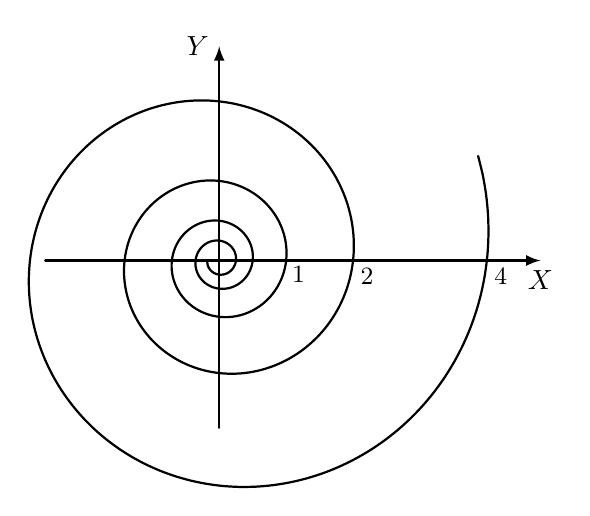
\begin{tikzpicture}[scale=0.85, >=latex, line cap=round, line join=round]
  % 座標軸
  \draw[thick, ->] (-2.6, 0) -- (4.8, 0) node[below] {$X$};
  \draw[thick, ->] (0, -2.5) -- (0, 3.2) node[left] {$Y$};
  % 螺線 r = 2^(\theta / 2\pi)
  \draw[thick, domain=-900:742, samples=400, smooth, variable=\t]
    plot (\t : {2^(\t/360)});
  % 交點刻度標記
  \node[below right, inner sep=1.5pt] at (1.02, -0.02) {\small $1$};
  \node[below right, inner sep=2pt] at (2.02, -0.02) {\small $2$};
  \node[below right, inner sep=2pt] at (4.02, -0.02) {\small $4$};
\end{tikzpicture}
\caption*{圖 3-1}\label{fig:b5-1-3-1}
\end{figure}

在上例中我們看到了「$r - 2^{\theta/2\pi} = 0$」與上圖「螺線」間的對應。\textbf{那麼我們問：一個 $r$ 與 $\theta$ 間的一般關係式}
\begin{equation}\label{eq:b5-1-3-2}
  g(r, \theta) = 0 \tag{2}
\end{equation}
\textbf{是否也正好對應一條極平面上的曲線？}

事實上這個對應在極座標是稍有一些困難的。

\medskip
\noindent\textbf{困難 1：}在上述例 1 $r - 2^{\theta/2\pi} = 0$ 中碰巧有 $r = 2^{\theta/2\pi} > 0$，我們未遭遇任何困難便得到該式與螺線間的良好對應。但一般情形下如果滿足 $g(r, \theta) = 0$ 中的某些 $r$ 會 $< 0$，我們怎樣處理？

\medskip
\noindent\textbf{〔例 2〕}\quad $r = \cos\theta$

\begin{center}
\renewcommand{\arraystretch}{1.6}
\setlength{\tabcolsep}{4.5pt}
\small
\begin{tabular}{c|cccccccccccccc}
$\theta$ & $\cdots\cdots$ & $0,$ & $\dfrac{\pi}{6},$ & $\dfrac{\pi}{4},$ & $\dfrac{\pi}{3},$ & $\dfrac{\pi}{2},$ & $\dfrac{2\pi}{3},$ & $\dfrac{3\pi}{4},$ & $\dfrac{5\pi}{6},$ & $\pi,$ & $\dfrac{5\pi}{4},$ & $\dfrac{3\pi}{2},$ & $\dfrac{7\pi}{4},$ & $2\pi$ \\[4pt]
\hline
$r$ & $\cdots\cdots$ & $1,$ & $\dfrac{\sqrt{3}}{2},$ & $\dfrac{\sqrt{2}}{2},$ & $\dfrac{1}{2},$ & $0,$ & $-\dfrac{1}{2},$ & $-\dfrac{\sqrt{2}}{2},$ & $-\dfrac{\sqrt{3}}{2},$ & $-1,$ & $-\dfrac{\sqrt{2}}{2},$ & $0,$ & $\dfrac{\sqrt{2}}{2},$ & $1$
\end{tabular}
\end{center}

當我們從 $\theta = 0$ 起開始描點，到 $\theta = \dfrac{\pi}{2}$ 前，$r$ 都 $> 0$，得到圖 3-2 中上半圓弧 $\wideparen{ABO}$。可是一旦 $\theta$ 過了 $\dfrac{\pi}{2}$，$r$ 值變負，例如 $\theta = \dfrac{2\pi}{3}$ 時 $r = -\dfrac{1}{2} < 0$，這時要是把點描到沿原來 $\dfrac{2\pi}{3}$ 角終邊 $\overrightarrow{OQ}$ 的逆方向 $\overrightarrow{OQ'}$ 距離極點 $\dfrac{1}{2}$ 處，則得點 $P$（如圖 3-2）。

\begin{figure}[H]
\centering
\begin{tikzpicture}[scale=3.2, >=latex, line cap=round, line join=round]
  % 座標軸
  \draw[thick, ->] (-0.5, 0) -- (1.45, 0) node[below] {$X$};
  \draw[thick, ->] (0, -0.65) -- (0, 0.78) node[left] {$Y$};
  \node[below left, inner sep=2pt] at (-0.02, -0.02) {$O$};

  % 圓 r = cos\theta (圓心 (0.5, 0)，半徑 0.5)
  \draw[thick] (0.5, 0) circle (0.5);

  % 第一象限描點射線
  \draw[->, thin] (0, 0) -- (30:1.18);
  \draw[->, thin] (0, 0) -- (45:1.12);
  \draw[->, thin] (0, 0) -- (60:0.95);

  % 第二象限射線 OQ (120度) 與第四象限逆方向射線 OQ' (300度)
  \draw[thick, ->] (0, 0) -- (120:0.78) node[right, xshift=1pt] {$Q$};
  \draw[thick] (0, 0) -- (300:0.5);
  \draw[thick, dashed, ->] (300:0.5) -- (300:0.82) node[right, xshift=1pt] {$Q'$};

  % 圓周各點標記
  \fill (1, 0) circle (0.018) node[below right, inner sep=2pt] {$A$};
  \fill (60:0.5) circle (0.018);
  \node[above left, inner sep=1.5pt] at (66:0.53) {$B$};
  \fill (300:0.5) circle (0.018);
  \node[below left, inner sep=2pt] at (292:0.52) {$P$};
  \fill (315:0.7071) circle (0.018) node[below right, inner sep=2pt] {$C$};

  % OP 長度 1/2 標記
  \node at (324:0.28) {\small $\dfrac{1}{2}$};
\end{tikzpicture}
\caption*{圖 3-2}\label{fig:b5-3-2}
\end{figure}

現在採用上述方式\textbf{只要在 $\theta$ 終邊的方向上 $r$ 值變負，便把點描到 $\theta$ 終邊的逆方向上}，即當 $\theta$ 從 $\dfrac{\pi}{2}$ 轉到 $\pi$ 時我們得到下半圓弧 $\wideparen{OCA}$。

綜合起來，當 $\theta$ 從 $0$ 到 $\pi$ 時，滿足
\[
  r = \cos\theta
\]
的點 $P[r, \theta]$ 描出了一個正圓。

採這例中的方式可彌補「困難 1」，換句話說，

\medskip
\noindent\textbf{規約：}\textbf{$r$ 若為負值，則 $[r, \theta]$ 所對應的點描在幅角為 $\theta + \pi$ 的終邊的方向上，其到原點的距離為 $|r|$。}

\medskip
如右圖 (3-3) 中 $\left[-3, \dfrac{\pi}{6}\right]$ 之點標在 $P$ 處。\textbf{$r$ 若為 $0$}，則不拘 $\theta$ 為何值，$[0, \theta]$ 所對應的點規定取成原點。

\begin{figure}[H]
\centering
\begin{tikzpicture}[scale=1.15, >=latex, line cap=round, line join=round]
  % 座標軸
  \draw[thick, ->] (-1.8, 0) -- (2.7, 0) node[right] {$X$};
  \draw[thick, ->] (0, -1.6) -- (0, 2.1) node[left] {$Y$};

  % 射線 \pi/6 與 \pi/6 + \pi
  \draw[thick] (0, 0) -- (30:2.35);
  \draw[thick] (0, 0) -- (210:2.15);

  % 角弧 \pi/6
  \draw[->] (0.75, 0) arc (0:30:0.75);
  \node at (16:1.30) {\footnotesize $\dfrac{\pi}{6}$};

  % 角弧 \pi/6 + \pi
  \draw[->] (0.42, 0) arc (0:210:0.42);
  \node at (135:0.92) {\small $\dfrac{\pi}{6} + \pi$};

  % 點 P 與距離 3 的弧線標示
  \fill (210:1.95) circle (1.5pt);
  \draw[thin] (0, 0) to[bend right=20] (210:1.95);
  \node[fill=white, inner sep=1pt] at (186:0.95) {\small $3$};
  \node[below left, inner sep=2pt] at (210:1.98) {$P$};
\end{tikzpicture}
\caption*{圖 3-3}\label{fig:b5-3-3}
\end{figure}

依照上述\textbf{規約}，我們知道了\textbf{兩個實數序對描述同一點 $P$ 的極座標之充要條件}，亦即

\medskip
\noindent\textbf{【命題 4】}\quad 當 $P \neq \text{原點}$ 時，$[r_1, \theta_1] = P = [r_2, \theta_2]$ 的充要條件是
\begin{equation}\label{eq:b5-1-3-3}
  \begin{cases}
    r_1 = r_2 \\
    \theta_1 = \theta_2 + 2n\pi
  \end{cases}
  \qquad \text{或} \qquad
  \begin{cases}
    r_1 = -r_2 \\
    \theta_1 = (\theta_2 + \pi) + 2n\pi
  \end{cases} \tag{3}
\end{equation}
其中 $n$ 是任意整數。

〔至於 $P = \text{原點}$ 時，$[r_1, \theta_1] = P = [r_2, \theta_2] \Longleftrightarrow r_1 = r_2 = 0$〕

(3) 式合併起來，可縮寫為
\[
  \begin{cases}
    r_1 = (-1)^k r_2 \\
    \theta_1 = \theta_2 + k\pi
  \end{cases}
\]
其中 $k$ 為任意整數。

\medskip
\noindent\textbf{作業 8}\quad 試描點畫出下列極平面上的軌跡圖形。
\begin{enumerate}[(i)]
  \item $r = \cos 2\theta$（四瓣）
  \item $r = \cos 3\theta$（三瓣）
\end{enumerate}
比較 (i), (ii) 與〔例 2〕$r = \cos\theta$ 三個軌跡各自要週而復始所須 $\theta$ 的最小範圍〔如 (i) 須 $\pi$\phantomsection\label{note:b5-ch1-p25-hw8}\footnote{【原書註記/校訂】：原書第 25 頁作業 8 提示印作「〔如 (i) 須 $\pi$〕」。按在 $r \le 0$ 規約下，(ii) 三瓣玫瑰線 $r = \cos 3\theta$ 因 $\cos 3(\theta + \pi) = -\cos 3\theta$，故 $\theta$ 僅須歷經長度為 $\pi$ 之區間（如 $[0, \pi]$）即可描出完整三瓣而週而復始；至於 (i) 四瓣玫瑰線 $r = \cos 2\theta$ 因 $\cos 2(\theta + \pi) = \cos 2\theta$，在 $[0, \pi]$ 上僅能描出兩瓣之長，須歷經 $2\pi$ 方能描出完整四瓣。原書括號提示中「(i)」應為「(ii)」之筆誤。}〕。

\medskip
\noindent\textbf{作業 9}\quad 試描點畫出下列極平面上的各個軌跡圖形
\begin{enumerate}[(i)]
  \item $r = \dfrac{2}{\cos\left(\theta - \dfrac{\pi}{3}\right)}$ \qquad （直線）
  \item $r = a, \ (a \neq 0)$ \qquad （圓）
  \item $r = \dfrac{2}{1 - \cos\theta}$ \qquad （拋物線）
\end{enumerate}

\medskip
\noindent\textbf{定義}\quad 對一個 $r, \theta$ 的關係式
\begin{equation}\label{eq:b5-1-3-4}
  g(r, \theta) = 0 \tag{4}
\end{equation}
考慮所有滿足這關係的 $r, \theta$ 所相應的點 $P[r, \theta]$，這些點 $P[r, \theta]$ 構成了極平面上的一個圖形 $\Gamma$。我們把 $\Gamma$ 稱為這個 $g(r, \theta) = 0$ 一式的軌跡，而 $g(r, \theta) = 0$ 稱為 $\Gamma$ 的一個\textbf{極座標方程式}或簡稱\textbf{極方程式}。

\medskip
\noindent\textbf{注意}
\begin{enumerate}[(i)]
  \item 根據甲段 $r \le 0$ 的規約，這個定義中，滿足 (2) 式的 $r, \theta$ 不受範圍的限制。
  \item $\Gamma$ 上一個點 $P$ 有許多極座標 $[r_1, \theta_1], [r_2, \theta_2], \cdots$（關係如 (2) 式\phantomsection\label{note:b5-ch1-p26-note}\footnote{【原書註記/校訂】：原書第 26 頁注意 (ii) 印作「（關係如 (2) 式）」，惟描述同一點 $P$ 之各組極座標 $[r_1, \theta_1], [r_2, \theta_2]$ 間的關係式實為第 25 頁【命題 4】之 (3) 式；此外下句「滿足的話，稱 $g(r, \theta) = 0$ 為良性的）」末尾多一右括號，轉錄時保留原貌並特此註明。}），當 $g(r, \theta) = 0$ 為 $\Gamma$ 的極方程式時\textbf{不一定}每一數對 $(r_1, \theta_1), (r_2, \theta_2), \cdots\cdots$ 都要滿足
  \[
    g(r_1, \theta_1) = g(r_2, \theta_2) = \cdots\cdots = 0.
  \]
  滿足的話，稱 $g(r, \theta) = 0$ 為\textbf{良性的}）

  如\textbf{〔例 1〕}螺線 $\Gamma : r = 2^{\theta/2\pi}$ 中，$P[1, 0]$ 是在 $\Gamma$ 上，而 $P$ 另有 $[1, 2\pi]$ 作為 $P$ 的極座標，但數對 $[1, 2\pi]$ 不滿足 $r = 2^{\theta/2\pi}$，意即
  \[
    1 \neq 2^{2\pi/2\pi} = 2
  \]
  \textbf{這是用極方程式描寫圖形的多種困難（如以後交點問題及對稱性判斷等）的起源}，這在下一節中我們要引入極圖觀點來詳細論述。
\end{enumerate}

\subsubsection*{乙、直線與圓的極方程式}\label{subsec:b5-1-3-b}

我們已知道如何從極方程式描點以求圖形，但實際上更需要的是要把一些基本圖形如直線，圓，二次錐線等以極方程式表示出來。

下面兩論例我們考慮直線與圓的情形：

\medskip
\noindent\textbf{【論例 3】}（直線的極方程式）

對直線 $L$ 的一般式
\begin{equation}\label{eq:b5-1-3-5}
  ax + by + c = 0 \tag{5}
\end{equation}
其中 $(x, y)$ 表直線 $L$ 上點的直角座標，根據 \S I-1 的變換式
\begin{equation}\label{eq:b5-1-3-6}
  \begin{cases}
    x = r\cos\theta \\
    y = r\sin\theta
  \end{cases}
  \qquad \text{〔註〕}\footnote{〔原書註〕：當初提出 (6) 式時我們並未考慮到 $r \le 0$ 的規約。因此，(7) 式中 $r \le 0$ 之解 $[r, \theta]$ 是否也在 $L$ 上呢？對於這個問題我們只須考慮 (6) 式在 $r \le 0$ 規約下是否仍然成立即可。從這一點我們又可看出我們為何要作 \S I-3 甲段那樣的規約了。（見習題 I-3 第 6 題）} \tag{6}
\end{equation}
其中 $[r, \theta]$ 表相應的極座標。顯然，以 (6) 式代入 (5) 式所得的
\[
  ar\cos\theta + br\sin\theta + c = 0
\]
\begin{equation}\label{eq:b5-1-3-7}
  \text{或} \qquad r(a\cos\theta + b\sin\theta) + c = 0 \tag{7}
\end{equation}
便是\textbf{直線的一般極座標方程式}。

若用\textbf{向量處理法線式的觀點}，自原點引 $L$ 的垂線 $OA$，$A$ 為垂足，$\vect{u}$ 為 $OA$ 線上，矢角 $\omega$ 在 $0$ 與 $\pi$ 之間的單位法向量。（$\omega$ 稱為法向角）。設 $p = \pm\overline{OA}$ 其 $+$ 或 $-$ 號依 $\vect{u}$ 與 $\overrightarrow{OA}$ 同向或異向而定，則
\[
  P[r, \theta] \in L
\]
的充要條件是
\[
  \overrightarrow{OP} \cdot \vect{u} = p
\]
亦即
\[
  r\cos(\theta - \omega) = p
\]
或寫成
\begin{equation}\label{eq:b5-1-3-8}
  r = \frac{p}{\cos(\theta - \omega)} \tag{8}
\end{equation}
這是一個\textbf{比較有幾何意義}的\textbf{直線的極座標方程式}。

\begin{figure}[H]
\centering
\begin{tikzpicture}[scale=1.15, >=latex, line cap=round, line join=round]
  % 座標軸
  \draw[thick, ->] (-1.2, 0) -- (4.2, 0) node[right] {$X$};
  \draw[thick, ->] (0, -1.0) -- (0, 3.8) node[above right, inner sep=1pt] {$Y$};
  \node[below left, inner sep=2pt] at (-0.02, -0.02) {$O$};

  % 定義法向角 \omega = 36度, p = 2.45
  \coordinate (A) at (36:2.45);
  % 直線 L 垂直於 OA (方向 126度 與 -54度)
  \draw[thick] ($(A) + (-54:1.75)$) -- ($(A) + (126:2.55)$);
  \node[above right, inner sep=2pt] at ($(A) + (-54:1.25)$) {$L$};

  % 垂足 A 與法線段 OA、單位法向量 u
  \draw[thick] (0, 0) -- (A);
  \draw[ultra thick, ->] (0, 0) -- (36:1.55);
  \node[below right, inner sep=2pt] at (33:1.52) {$\vect{u}$};
  \node[below right, inner sep=2pt] at (35:2.05) {$p$};
  \node[above right, inner sep=2pt] at (A) {$A$};

  % 直線上點 P[r, \theta] (\theta = 68度, r = 2.45 / cos(32度) = 2.889)
  \coordinate (P) at (68:2.889);
  \draw[thick] (0, 0) -- (P);
  \node[above right, inner sep=2pt] at (P) {$P[r, \theta]$};

  % 角弧 \omega (0 到 36度)
  \draw (0.48, 0) arc (0:36:0.48);
  \node at (18:0.66) {\small $\omega$};

  % 角弧 \theta (0 到 68度)
  \draw[->] (0.92, 0) arc (0:68:0.92);
  \node at (16:1.14) {\small $\theta$};

  % 角弧 \theta - \omega (36 到 68度)
  \draw (36:1.68) arc (36:68:1.68);
  \node at (52:2.02) {\small $\theta - \omega$};
\end{tikzpicture}
\end{figure}

\noindent\textbf{特殊情形：}
\begin{enumerate}[(i)]
  \item 當 $L$ 平行於極軸時，$\omega = \dfrac{\pi}{2}$，故得
  \[
    r = \frac{p}{\cos\left(\theta - \dfrac{\pi}{2}\right)} = \frac{p}{\sin\theta}
  \]
  即 \qquad $r\sin\theta = p$
  \item 當 $L$ 垂直於極軸時，$\omega = 0$，故得
  \[
    r\cos\theta = p.
  \]
\end{enumerate}

\medskip
\noindent\textbf{【論例 4】}（圓的極方程式）

\noindent\textbf{解}\quad 考慮一圓 $\Gamma$，圓心 $C$ 之極座標為 $[\rho, \alpha]$，半徑為 $a$，則
\[
  \text{「}P[r, \theta] \in \Gamma\text{」}
\]
的充要條件為
\[
  \text{「}\overline{CP} = a \text{（即 } \overline{CP}^2 = a^2\text{）」}
\]
根據餘弦定律，這充要條件可寫成
\begin{equation}\label{eq:b5-1-3-9}
  r^2 + \rho^2 - 2\rho r\cos(\theta - \alpha) = a^2 \tag{9}
\end{equation}
這便是\textbf{圓的極方程式}。\hfill$\#$

\begin{figure}[H]
\centering
\begin{tikzpicture}[scale=1.15, >=latex, line cap=round, line join=round]
  % 極點 O 與極軸 OX
  \coordinate (O) at (0, 0);
  \node[below left, inner sep=2pt] at (O) {$O$};
  \draw[thick, ->] (O) -- (5.5, 0) node[above, yshift=2pt] {$X$} node[below, yshift=-2pt, xshift=-6pt] {\small 極軸};

  % 圓心 C[\rho, \alpha] (\alpha = 18度, \rho = 3.65, 半徑 a = 1.25)
  \coordinate (C) at (18:3.65);
  \draw[thick] (C) circle (1.25);
  \fill (C) circle (1.5pt);
  \node[below, yshift=-3pt, xshift=4pt] at (C) {$C[\rho, \alpha]$};

  % 圓上點 P[r, \theta]
  \coordinate (P) at ($(C) + (92:1.25)$);
  \fill (P) circle (1.5pt);
  \node[above, yshift=2pt] at (P) {$P[r, \theta]$};

  % 連線 OC, OP 與虛線半徑 CP
  \draw[thick] (O) -- (C);
  \draw[thick] (O) -- (P) node[midway, above left, inner sep=2pt] {$r$};
  \draw[thick, dashed] (C) -- (P) node[midway, right, xshift=2pt] {$a$};

  % 角弧 \alpha 與 \theta - \alpha
  \draw[->] (1.00, 0) arc (0:18:1.00);
  \node at (9:1.24) {\small $\alpha$};
  \draw (18:1.25) arc (18:36.8:1.25);
  \node at (26.5:1.68) {\footnotesize $\theta - \alpha$};
\end{tikzpicture}
\end{figure}

\noindent\textbf{注意：}在這兩論例中，直線或圓上一點 $P$ 的任何極座標 $[r, \theta]$，$[-r, \theta + \pi]$，$[r, \theta + 2\pi]\cdots\cdots$ 等中每一數對都分別滿足它們的極方程式 (8), (9) 式，其道理留當\textbf{作業}。這樣的極方程式，我們稱為\textbf{良性的極方程式}，這現象不是始終都成立的（如 $r = 2^{\theta/2\pi}$）。\textbf{但當它成立時，許多用極方程式討論的可能的疵漏都可避免}（見下面\textbf{作業}及下節交點問題）\phantomsection\label{note:b5-ch1-p28-fn}\footnote{〔原書註〕：此處我們視圓 $x^2 + y^2 = a^2$ 的極方程式為 $r^2 = a^2$，因為開方會去掉 $r = -a$ 使得剩下的方程式 $r = a$ 不為良性。（【編按】：原書第 28 頁頁底印有此則「〔註〕」，惟正文中未標註對應之「〔註〕」號，依文義係補充說明圓之良性極方程式，故綴於此段末尾。）}。

\medskip
\noindent\textbf{〔例 3〕}\quad 設一圓通過以下列的直角座標表其位置的三個點
\[
  P_1(0, 0), \quad P_2(1, 0), \quad P_3(0, 2)
\]
求此圓的極方程式。

\medskip
\noindent\textbf{解}
\begin{enumerate}[(i)]
  \item 我們的方法是找出這三點的極座標
  \[
    P_1 = (0, 0) = [0, 0], \qquad P_2 = (1, 0) = [1, 0],
  \]
  \[
    P_3 = (0, 2) = \left[2, \frac{\pi}{2}\right]
  \]
  然後將這些數對分別代入圓的一般方程式
  \begin{equation}\label{eq:b5-1-3-10}
    r^2 + \rho^2 - 2\rho r\cos(\theta - \alpha) = a^2 \qquad (\text{取 } a > 0) \tag{10}
  \end{equation}
  得：〔這些數對為什麼滿足 (10) 式？〕
  \[
    \begin{cases}
      \rho^2 = a^2 \\
      1 + \rho^2 - 2\rho\cos\alpha = a^2 \\
      4 + \rho^2 - 4\rho\cos\left[\dfrac{\pi}{2} - \alpha\right] = a^2
    \end{cases}
  \]
  簡化得 $1 - 2a\cos\alpha = 0$，及 $1 - a\sin\alpha = 0$\phantomsection\label{note:b5-ch1-p29-ex3}\footnote{【原書註記/校訂】：原書第 29 頁由聯立方程組 $\rho^2 = a^2$（取 $\rho = a > 0$）消去常數項後，直接將 $\rho$ 寫作 $a$ 而得 $1 - 2a\cos\alpha = 0$ 及 $1 - a\sin\alpha = 0$，並代入 (10) 式化為 $r = 2a\cos(\theta - \alpha)$。}

  代入 (10) 式後可化簡得
  \begin{align*}
    r &= 2a\cos(\theta - \alpha) \\
      &= (2a\cos\alpha)\cos\theta + (2a\sin\alpha)\sin\theta
  \end{align*}
  亦即 \qquad $r = \cos\theta + 2\sin\theta$ \qquad 〔註〕\footnote{〔原書註〕：在得到此式前我們將兩端消去了一個 $r$ 但可以驗得這個操作並未損失原點之根。}

  \item 但這方法為什麼是正確的？換句話說為什麼上述數對會滿足 (10) 式？例如 $P_3$ 有其他極座標 $\left[2, \dfrac{\pi}{2} + 2\pi\right], \left[-2, \dfrac{\pi}{2} - \pi\right], \cdots$ 等，我們知道 $P_3$ 在圓上時，只知 $P_3$ 的各極座標中\textbf{有一個}它的數對會滿足 (10) 式。幸好本例前的「注意」告訴我們若 $P$ 在圓上，則 $P$ 的每一個極座標所含的數對都會滿足 (10) 式，故上述討論無誤。\hfill$\#$
\end{enumerate}

從最後這個例子中，我們注意到：以前採用直角座標方程式描述曲線時從不會發生的問題，現在採用極座標時便有了困難，換句話說，一般時候
\[
  g(r, \theta) = 0
\]
所代表的軌跡上的一點 $P = [r_0, \theta_0] = [-r_0, \theta_0 + \pi] = [r_0, \theta_0 + 2\pi] = \cdots\cdots$ 中只知至少有一組數對是滿足 $g(r, \theta) = 0$，譬如可能 $g(r_0, \theta_0) = 0$，但 $g(-r_0, \theta_0 + \pi) \neq 0, \ g(r_0, \theta_0 + 2\pi) \neq 0$。

% =========================================================================
% 習題 I-3
% =========================================================================
\subsubsection*{習題 I-3}\label{sec:b5-ex1-3}

\begin{enumerate}[1.]
  \item 求下列直線之極方程式
  \begin{enumerate}[(a)]
    \item 斜率為 $3$，$Y$ 截距為 $-2$
    \item 斜率為 $-2$，到原點距離為 $5$（兩解）
    \item $X, Y$ 兩軸截距分別為 $2, -6$。
  \end{enumerate}

  \item 求下列圓之極方程式
  \begin{enumerate}[(a)]
    \item 圓心在 $(-2, 1)$，半徑為 $5$
    \item 通過 $(0, 0), (u, 0), (0, v)$ 三點 $(u, v \neq 0)$
    \item 以 $(4, 1), (2, 3)$ 連線為直徑
  \end{enumerate}

  \item 設 $P[r_0, \theta_0]$ 在直線
  \[
    r = \frac{p}{\cos(\theta - \omega)}
  \]
  上，是否必然可得
  \[
    r_0 = \frac{p}{\cos(\theta_0 - \omega)}\text{？}
  \]
  解釋其道理。

  \item 想求一直線與一圓的交點，是否解其相應的極方程式
  \[
    \begin{cases}
      r = \dfrac{p}{\cos(\theta - \omega)} \\[8pt]
      r^2 + \rho^2 - 2\rho r\cos(\theta - \alpha) = a^2
    \end{cases}
  \]
  必可獲得所有交點？其道理何在？

  \item 求一通過 $(0, 1)$ 而與 $2x + \sqrt{3}y = 1$ 相切之圓的極方程式。

  \item 在論例 3 中我們其實已經得到一個把直角座標方程式變換成極方程式的一般方法。試將下列事實顯示出來：
  \begin{enumerate}[(a)]
    \item $(x, y)$ 與 $[r, \theta]$ 表相同點的充要條件是
    \[
      \begin{cases}
        x = r\cos\theta \\
        y = r\sin\theta
      \end{cases}
    \]
    特別注意上式中 $r \le 0$ 也成立。
    \item 若圖形 $\Gamma$ 的直角座標方程式是 $f(x, y) = 0$，則它的極座標方程式是 $f(r\cos\theta, r\sin\theta) = 0$，其逆亦真。
    \item 由上述方法得來的極方程式 $f(r\cos\theta, r\sin\theta) = 0$ 是良性的，即，若 $P$ 在 $f(r\cos\theta, r\sin\theta) = 0$ 之圖形上，則 $P$ 的每一個極座標 $[r_0, \theta_0]$ 必然都滿足 $f(r_0\cos\theta_0, r_0\sin\theta_0) = 0$。
  \end{enumerate}

  \item 試從圓的直角座標方程式再導出圓的極方程式
  \[
    r^2 + \rho^2 - 2\rho r\cos(\theta - \alpha) = a^2.
  \]
  從這個導引過程，第 6 題直接告訴我們：圓方程式是「良性的」方程式。

  \item[\textbf{*8.}]
  \begin{enumerate}[(a)]
    \item 已知極平面上兩點 $A$、$B$，其中 $A$ 為二直線
    \[
      r\cos\left(\theta - \frac{\pi}{6}\right) = 3, \quad r\sin\theta = 3 \text{ 的交點，} B \text{ 為 } \left[2, \frac{5\pi}{6}\right]\text{；}
    \]
    試求出通過 $A, B$ 兩點的直線極方程式
    \item 由 (a) 所得直線 $AB$ 有一動點 $P[r_1, \theta_1]$，現以 $OP$ 線段為一邊，作正三角形 $\triangle OPQ$，（$O$ 為極），試求出頂點 $Q$ 之軌跡決定的極方程式。
  \end{enumerate}

  \item 試求出過三點 $[0, 0], [\alpha, 0], \left[\beta, \dfrac{\pi}{2}\right]$ 之圓的極方程式。$(\alpha\beta \neq 0)$，
  \[
    [r = \alpha\cos\theta + \beta\sin\theta]
  \]

  \item[\textbf{*10.}] 試利用習題 I-1 第 5 題的解法導出平面上三點 $[r_1, \theta_1], [r_2, \theta_2], [r_3, \theta_3]$ 點所決定三角形的面積大小。
\end{enumerate}
% =========================================================================
% §I-4 交點問題 (Pages 31--45)
% =========================================================================
\subsection{交點問題}\label{sec:b5-1-4}

\subsubsection*{甲、困難的提出}

用極座標方程式來描寫曲線，還存在著其他一些困難。

\medskip
\noindent\textbf{〔例 1〕}考慮兩方程式
\begin{equation}
\begin{cases}
r = 2^{\theta / 2\pi} \\[4pt]
\theta = \dfrac{2\pi}{3}
\end{cases}
\tag{1}
\end{equation}

\begin{figure}[H]
\centering
\begin{tikzpicture}[scale=1.18, >=Stealth]
  % Axes
  \draw[->, thick] (-2.6, 0) -- (2.8, 0) node[right] {$X$};
  \draw[->, thick] (0, -2.4) -- (0, 2.5) node[left] {$Y$};

  % Line l: \theta = 2\pi/3 (120 deg and -60 deg)
  \draw[thick] (120:2.5) -- (-60:2.4) node[right, pos=0.92] {$\ell : \theta = \dfrac{2\pi}{3}$};

  % Spiral r = 2^{\theta / 2\pi}
  \draw[thick, domain=-420:495, samples=300, smooth, variable=\t]
    plot (\t : {0.70 * exp(\t/360 * ln(2.25))});

  % Intersection points on 120 deg ray (with short leader lines to clear space)
  \fill (120:0.408) circle (1.5pt);
  \draw[thin, gray] (120:0.408) -- (152:0.85) node[left, inner sep=1pt, black, font=\footnotesize] {$P_{-1}$};

  \fill (120:0.917) circle (1.5pt);
  \draw[thin, gray] (120:0.917) -- (140:1.45) node[left, inner sep=1pt, black, font=\footnotesize] {$P_0$};

  \fill (120:2.064) circle (1.5pt);
  \node[above right=2pt, font=\small] at (120:2.064) {$P_1$};

  % Intersection points on -60 deg ray
  \fill (-60:0.612) circle (1.5pt);
  \fill (-60:1.376) circle (1.5pt);

  % Label for spiral with pointer
  \draw[<-, thin] (50:1.61) .. controls (53:1.82) and (48:1.92) .. (50:2.12)
    node[above right, inner sep=1pt] {$r = 2^{\theta / 2\pi}$};
\end{tikzpicture}
\caption*{圖 4-1}
\end{figure}

恰得一公解\quad $r = 2^{\frac{1}{3}}$，$\theta = \dfrac{2\pi}{3}$

記 $P_0 = \left[2^{\frac{1}{3}}, \dfrac{2\pi}{3}\right]$，但兩式在極平面上一表螺狀線〔見 \S I-3 例 1〕，一表幅角為 $\dfrac{2\pi}{3}$ 的終邊。（其實依照上段「規約」，$r$ 值可負，$\theta = \dfrac{2\pi}{3}$ 應推廣為整條直線 $l$），兩線卻有無限多的交點，如圖 4-1。\hfill$\#$

\medskip
換句話說，由所給聯立極座標方程式 (1) 所求得的公解，未能示出兩相應軌跡的所有交點。

\medskip
\noindent\textbf{〔例 2〕}討論兩方程式的公解及相應軌跡的交點
\begin{equation}
\begin{cases}
r = 2^{\theta / 2\pi} \\[4pt]
r = 2^{(\theta + 2\pi) / 2\pi}
\end{cases}
\tag{2}
\end{equation}

\noindent\textbf{解}\quad 欲求其公解，必要求下式成立
\[
2^{\theta / 2\pi} = 2^{(\theta + 2\pi) / 2\pi}
\]
則得
\[
\theta / 2\pi = (\theta + 2\pi) / 2\pi \qquad \text{〔因指數函數為單調〕}
\]
即
\[
\theta = \theta + 2\pi
\]
顯然沒有 $\theta$ 能滿足上式，故所給聯立方程式 (2) 無解。

可是 $r = 2^{\theta / 2\pi}$ 與 $r = 2^{(\theta + 2\pi) / 2\pi}$ 兩式竟然描出了極平面上同一螺狀軌跡。（圖 4-2）\hfill$\#$

\begin{figure}[H]
\centering
\begin{tikzpicture}[scale=1.0, >=Stealth]
  \draw[->, thick] (-2.5, 0) -- (2.8, 0) node[below right] {$X$};
  \draw[->, thick] (0, -2.2) -- (0, 2.4) node[right] {$Y$};
  \draw[thick, domain=-420:540, samples=300, smooth, variable=\t]
    plot (\t : {0.58 * exp(\t/360 * ln(2.05))});
\end{tikzpicture}
\caption*{圖 4-2\quad 重合的兩個螺狀線}
\end{figure}

這兩個例子顯示極平面軌跡方程無法良好地描述其上的曲線，換句話說：

\medskip
\noindent\textbf{困難 2}：\textbf{代數上聯立方程式的公解，原對應於幾何上圖形間的交點，可是這一重要的轉化關係採用極座標時卻發生了困難。}

\medskip
其實這一困難要追溯的話，原起自平面上同一個點不只對應一個極座標，換句話說，\textbf{極座標不是一個足夠良好的座標}，從這裏引出的困難，除了交點問題外，還有對稱性問題等一些伴隨而來的副作用。可是極座標在描述某些現象時又不失為好的描述〔例如\underline{牛頓}採二次曲線的極座標表示，再利用微分，而自\underline{刻卜勒}三大觀測結果導出萬有引力定律，這是科學史上的一件大事〕。下一段我們將引入\textbf{極圖的觀點}，\textbf{澄清極座標各種困難的基本癥結}。

\subsubsection*{乙、極圖（polar chart）的觀點}

以下所謂 \textbf{$(\theta, r)$-平面}意指平常的座標平面，但現在以 $\theta$ 表橫座標，$r$ 表縱座標。〔見下圖 4-3〕

如果自 $g(r, \theta) = 0$ 中可解得
\[
r = p(\theta)
\]
我們先\textbf{不在極平面上而在 $(\theta, r)$-平面上}畫出 $r$ 表以 $\theta$ 的函數圖形，〔亦即把 $\theta$ 當成 $t$，把 $r$ 當成 $u$ 在 $(t, u)$-平面上畫 $u = p(t)$ 的函數圖形〕。例如 $r = \cos\theta$ 時我們畫出〔參考第三冊，習題 2-2〕

\begin{figure}[H]
\centering
\begin{tikzpicture}[scale=0.85, >=Stealth]
  \draw[->, thick] (-4.5, 0) -- (8.2, 0) node[right] {$\theta$};
  \draw[->, thick] (0, -1.5) -- (0, 1.8) node[right] {$r$};
  \node[below left] at (0, 0) {$O$};
  \draw[thick, domain=-4.0:7.5, samples=200, smooth, variable=\x]
    plot (\x, {0.85 * cos(\x r)});
  \draw[<-, thin] (5.85, {0.85 * cos(5.85 r)}) .. controls (6.05, 1.15) and (6.25, 1.25) .. (6.55, 1.35)
    node[right] {$r = \cos\theta$};
  \node[below] at (0, -1.5) {$(\theta, r)$-平面};
\end{tikzpicture}
\caption*{圖 4-3\quad 〔在 $(\theta, r)$-平面上橫座標表 $\theta$，縱座標表 $r$〕}
\end{figure}

今取一函數
\[
\gamma(\theta, r) \equiv (r\cos\theta, r\sin\theta)
\]
$\gamma$ 為從 $(\theta, r)$-平面到 $(x, y)$-平面上的一個映射，其中
\[
\begin{cases}
x = r\cos\theta \\[4pt]
y = r\sin\theta
\end{cases}
\]
如圖 4-4

\begin{figure}[H]
\centering
\begin{tikzpicture}[scale=0.95, >=Stealth]
  % Left: (\theta, r)-plane
  \draw[->, thick] (-1.8, 0) -- (3.1, 0) node[right] {$\theta$};
  \draw[->, thick] (0, -2.0) -- (0, 2.3) node[right] {$r$};
  \node[below left] at (-0.15, -0.05) {$0$};

  % Ticks on axes
  \foreach \x in {0.8, 1.8} {
    \fill (\x, 0) circle (1.5pt);
  }
  \foreach \y in {-1.5, -0.75, 0.75, 1.5} {
    \fill (0, \y) circle (1.5pt);
  }

  % Vertical line at \theta = 3\pi/4 (represented at x = 1.8)
  \draw[thick] (1.8, -1.9) -- (1.8, 2.0);

  % Three points in (\theta, r)-plane
  \coordinate (A) at (0.8, 1.5);
  \coordinate (B) at (1.8, 0.75);
  \coordinate (C) at (1.8, -1.5);

  \fill (A) circle (1.8pt);
  \node[below right=1pt, font=\footnotesize] at (A) {$(\theta, r)$};

  \fill (B) circle (1.8pt);
  \node[above left=2pt, fill=white, inner sep=1pt, font=\scriptsize] at (1.76, 0.78) {$\left(\dfrac{3\pi}{4}, 1\right)$};

  \fill (C) circle (1.8pt);
  \node[right=3pt, font=\scriptsize] at (1.8, -1.5) {$\left(\dfrac{3\pi}{4}, -2\right)$};

  \node[below] at (0.3, -2.1) {$(\theta, r)$-平面};

  % Middle mapping arrow \gamma
  \draw[->, thick] (3.6, 0) -- node[above] {$\gamma$} (4.6, 0);

  % Right: (x, y)-plane
  \begin{scope}[xshift=7.1cm]
    \draw[->, thick] (-2.0, 0) -- (2.8, 0) node[right] {$x$};
    \draw[->, thick] (0, -1.9) -- (0, 2.3) node[right] {$y$};

    % Ticks on y-axis
    \foreach \y in {0.75, 1.5} {
      \fill (0, \y) circle (1.5pt);
    }

    % Point A' in 1st quadrant (angle ~ 65 deg, radius 1.65)
    \coordinate (Ap) at (65:1.65);
    \draw[thick] (0, 0) -- node[left=1pt, pos=0.65] {$r$} (Ap);
    \fill (Ap) circle (1.8pt);
    \draw (0.38, 0) arc[start angle=0, end angle=65, radius=0.38];
    \node[right=1pt] at (32:0.42) {$\theta$};

    % Line at 3\pi/4 (135 deg and -45 deg)
    \draw[thick] (135:1.2) -- (-45:1.9);
    \coordinate (Bp) at (135:0.75);
    \coordinate (Cp) at (-45:1.5);
    \fill (Bp) circle (1.8pt);
    \fill (-45:0.75) circle (1.5pt);
    \fill (Cp) circle (1.8pt);

    \node[below] at (0.5, -1.9) {$(x, y)$-平面};
  \end{scope}

  % Curved arrows showing the mapping of the 3 points (arising cleanly without crossing labels)
  \draw[->, thick] (A) .. controls (2.4, 2.45) and (5.5, 2.35) .. (Ap);
  \draw[->, thick] (B) .. controls (2.4, 1.55) and (5.0, 1.35) .. (Bp);
  \draw[->, thick] (C) .. controls (2.4, -2.25) and (5.5, -2.15) .. (Cp);
\end{tikzpicture}
\caption*{圖 4-4}
\end{figure}

這個函數 $\gamma$ 稱為平面上的極圖映射，或簡稱極圖。

如果我們在 $(x, y)$-平面上，考慮極座標為 $[r, \theta]$ 的點 $P$，則
\[
[r, \theta] = P = (r\cos\theta, r\sin\theta) \in (x, y)\text{-平面}
\]
亦即得到
\[
\gamma(\theta, r) = [r, \theta] \in (x, y)\text{-平面}
\]
換句話說，$\gamma$ 把在 $(\theta, r)$-平面上\textbf{橫座標為 $\theta$，縱座標為 $r$} 的點帶到 $(x, y)$-平面上\textbf{極座標為 $[r, \theta]$} 的點。亦即 \textbf{$\gamma$ 賦予 $(x, y)$-平面上的點 $P$ 新的一個數對 $[r, \theta]$}，這個數對就是 $P$ 點的極座標，因此我們稱 $\gamma$ 為極圖映射，也因此 $(x, y)$-平面在配置極圖 $\gamma$ 後，實際上就有了極座標，而稱為極平面。

由於 $\gamma(P_1) = \gamma(P_2) \Longleftrightarrow [r_1, \theta_1] = [r_2, \theta_2]$，依據\textbf{甲段所述} $[r_1, \theta_1] = [r_2, \theta_2]$ 的充要條件，我們知：

\medskip
\noindent\textbf{【命題 4】}設 $(\theta, r)$-平面上一點 $P_1(\theta_1, r_1)$，若 $r_1 \neq 0$，則另一點 $P_2(\theta_2, r_2)$ 經極圖 $\gamma$ 映射後會與 $P_1(\theta_1, r_1)$ 得同一像點 $P'$ 的充分必要條件是
\[
\begin{cases}
r_2 = r_1 \\[4pt]
\theta_2 = \theta_1 + 2n\pi
\end{cases}
\qquad \text{或} \qquad
\begin{cases}
r_2 = -r_1 \\[4pt]
\theta_2 = (\theta_1 + \pi) + 2n\pi
\end{cases}
\]
其中 $n$ 為任意整數。

上式合併起來可寫成
\[
\begin{cases}
r_2 = (-1)^k r_1 \\[4pt]
\theta_2 = \theta_1 + k\pi
\end{cases}
\]
其中 $k$ 為任意整數。

若 $r_1 = 0$，則 $\gamma(P_1) = \gamma(P_2) \Longleftrightarrow r_2 = 0$。

\begin{figure}[H]
\centering
\begin{tikzpicture}[scale=0.95, >=Stealth]
  % Left: (\theta, r)-plane
  % Let 1.15 units on x-axis = \pi
  \draw[->, thick] (-2.9, 0) -- (5.3, 0) node[right] {$\theta$};
  \draw[->, thick] (0, -2.0) -- (0, 2.3) node[right] {$r$};
  \node[below left] at (0, 0) {$O$};

  % Vertical grid lines at multiples of \pi
  \foreach \k/\lbl in {-2/-2\pi, -1/-\pi, 1/\pi, 2/2\pi, 3/3\pi, 4/4\pi} {
    \draw[thin] ({1.15*\k}, -1.8) -- ({1.15*\k}, 2.0);
    \node[below left, font=\footnotesize, inner sep=1pt] at ({1.15*\k}, -0.05) {$\lbl$};
  }

  % Braces on r-axis showing height 3 and depth 3
  \node[left=1pt, font=\footnotesize] at (0, 0.5) {$3\Big\{$};
  \node[right=1pt, font=\footnotesize] at (0, -0.5) {$\Big\}3$};

  % Points P_{-1}, P_0, P_1 at r = 3 (y = 1.0)
  \fill ({1.15*(-1.333)}, 1.0) circle (1.6pt) node[below=1pt, font=\footnotesize] {$P_{-1}$};
  \fill ({1.15*0.667}, 1.0) circle (1.6pt) node[below=1pt, font=\footnotesize] {$P_0$};
  \node[above=3pt, fill=white, inner sep=1pt, font=\scriptsize] at ({1.15*0.667}, 1.04) {$\left(\dfrac{2\pi}{3}, 3\right)$};
  \fill ({1.15*2.667}, 1.0) circle (1.6pt) node[below=1pt, font=\footnotesize] {$P_1$};

  % Points \overline{P}_{-1}, \overline{P}_0, \overline{P}_1 at r = -3 (y = -1.0)
  \fill ({1.15*(-0.333)}, -1.0) circle (1.6pt) node[below=1pt, font=\footnotesize] {$\overline{P}_{-1}$};
  \fill ({1.15*1.667}, -1.0) circle (1.6pt) node[below=1pt, font=\footnotesize] {$\overline{P}_0$};
  \fill ({1.15*3.667}, -1.0) circle (1.6pt) node[below=1pt, font=\footnotesize] {$\overline{P}_1$};

  % Middle arrow \gamma
  \draw[->, thick] (5.9, 0) -- node[above] {$\gamma$} (6.9, 0);

  % Right: (X, Y)-plane
  \begin{scope}[xshift=9.2cm]
    \draw[->, thick] (-2.0, 0) -- (2.0, 0) node[right] {$X$};
    \draw[->, thick] (0, -1.8) -- (0, 2.3) node[right] {$Y$};
    \node[below left] at (0, 0) {$O$};

    \draw[ultra thick] (0, 0) -- node[below left=1pt, pos=0.5, font=\footnotesize] {$3$} (120:1.35);
    \fill (120:1.35) circle (1.8pt) node[above left=1pt, font=\small] {$P'\left[3, \dfrac{2\pi}{3}\right]$};
  \end{scope}
\end{tikzpicture}
\caption*{圖 4-5\quad 〔左圖 $(\theta, r)$-平面上諸點 $P_i$ 及 $\overline{P}_j$ 等經 $\gamma$ 後都映至同一像點 $P'$〕}
\end{figure}

另一方面在極圖映射之下，上述 $(\theta, r)$-平面上 $r = \cos\theta$ 的波浪狀函數圖形現在變成了 $(x, y)$-平面（今為極平面）上一個週而復始的圓，其週期為 $\pi$〔參看 \S I-3 例 2〕

\begin{figure}[H]
\centering
\begin{tikzpicture}[scale=0.9, >=Stealth]
  % Left: (\theta, r)-plane
  \draw[->, thick] (-2.0, 0) -- (5.8, 0) node[right] {$\theta$};
  \draw[->, thick] (0, -1.5) -- (0, 1.8) node[right] {$r$};
  \node[below left] at (0, 0) {$O$};

  \draw[thick, domain=-1.7:5.3, samples=160, smooth, variable=\x]
    plot (\x, {0.85 * cos(\x r)});

  % Points P_1, P_2, P_3
  \fill (0, 0.85) circle (1.6pt) node[above right, font=\footnotesize] {$P_1$};
  \fill (1.571, 0) circle (1.6pt) node[above right=2pt, font=\footnotesize] {$P_2$};
  \fill (2.356, {-0.85*0.707}) circle (1.6pt) node[below left, font=\footnotesize] {$P_3$};

  % Label \Lambda: r = \cos\theta
  \draw[<-, thin] (4.0, {0.85 * cos(4.0 r)}) .. controls (4.1, 0.7) and (4.2, 0.8) .. (4.4, 1.05)
    node[right, font=\footnotesize] {$\Lambda : r = \cos\theta$};

  \node[below, font=\footnotesize] at (0, -1.5) {$(\theta, r)$-平面};

  % Middle arrow \gamma
  \draw[->, thick] (6.5, 0) -- node[above] {$\gamma$} (7.3, 0);

  % Right: (x, y)-plane
  \begin{scope}[xshift=9.0cm]
    \draw[->, thick] (-1.0, 0) -- (3.2, 0) node[right] {$x$};
    \draw[->, thick] (0, -1.5) -- (0, 1.8) node[right] {$y$};
    \node[below left] at (0, 0) {$O$};

    % Circle centered at (0.65, 0) with radius 0.65
    \draw[thick] (0.65, 0) circle (0.65);

    \fill (1.3, 0) circle (1.6pt) node[above right, font=\footnotesize] {$P'_1$};
    \fill (0, 0) circle (1.6pt) node[above left, font=\footnotesize] {$P'_2$};
    \fill (0.65, -0.65) circle (1.6pt) node[below right, font=\footnotesize] {$P'_3$};

    % Pointer to circle
    \draw[<-, thin] (0.85, 0.62) .. controls (0.95, 0.85) and (1.05, 0.9) .. (1.2, 1.1)
      node[right, align=left, font=\scriptsize] {極座標 $[r, \theta]$ 滿足\\$r = \cos\theta$ 的點的軌跡\\$\Lambda' = \gamma(\Lambda)$};

    \node[below, font=\footnotesize] at (1.1, -1.5) {$(x, y)$-平面〔極平面〕};
  \end{scope}
\end{tikzpicture}
\caption*{圖 4-6}
\end{figure}

實際上，$(\theta, r)$-平面上的點與數對 $(\theta, r)$〔$\theta$ 表點的橫座標，$r$ 表點的縱座標〕之間才真正是良好的一一對應，也因此 $r = \cos\theta$ 與它在 $(\theta, r)$-平面上所繪的波浪狀函數圖形 $\Lambda$ 是毫無疵漏。至於用極座標 $[r, \theta]$ 在極平面上以 $r = \cos\theta$ 表達的圖形\underline{其實是 $\Lambda$ 經極圖映射 $\gamma$ 後}\underline{的像集所構成的圖形 $\Lambda'$}，換句話說
\[
\Lambda' = \gamma(\Lambda).\footnote{〔原書頁底註〕$\Lambda$ 讀音 Lambda 為 $\lambda$ 之大寫。}
\]

\medskip
\noindent\textbf{〔例 3〕}$r = 2^{\theta / 2\pi}$

\begin{figure}[H]
\centering
\begin{tikzpicture}[scale=0.95, >=Stealth]
  % Left: (\theta, r)-plane
  \draw[->, thick] (-1.8, 0) -- (3.2, 0) node[right] {$\theta$};
  \draw[->, thick] (0, -1.5) -- (0, 2.2) node[right] {$r$};
  \draw[thick, domain=-1.5:1.5, samples=100, smooth, variable=\x]
    plot (\x, {0.65 * exp(0.75 * \x)});
  \draw[<-, thin] (1.1, {0.65 * exp(0.75 * 1.1)}) .. controls (1.4, 1.35) and (1.6, 1.45) .. (1.9, 1.85)
    node[right] {$\Lambda$};
  \node[below, font=\footnotesize] at (0.3, -1.5) {$(\theta, r)$-平面};

  % Middle arrow \gamma
  \draw[->, thick] (4.1, 0) -- node[above] {$\gamma$} (5.1, 0);

  % Right: (x, y)-plane
  \begin{scope}[xshift=7.8cm]
    \draw[->, thick] (-2.2, 0) -- (2.5, 0) node[right] {$x$};
    \draw[->, thick] (0, -1.5) -- (0, 2.2) node[right] {$y$};
    \draw[thick, domain=-420:490, samples=260, smooth, variable=\t]
      plot (\t : {0.48 * exp(\t/360 * ln(2.05))});
    \draw[<-, thin] (45:0.95) .. controls (45:1.25) and (40:1.35) .. (42:1.65)
      node[right] {$\Lambda' = \gamma(\Lambda)$};
    \node[below, font=\footnotesize] at (0.3, -1.5) {$(x, y)$-平面};
  \end{scope}
\end{tikzpicture}
\caption*{圖 4-7}
\end{figure}

$r = 2^{\theta / 2\pi}$ 在 $(\theta, r)$-平面上是單調上升的曲線 $\Lambda$，在極平面上所有滿足它的點 $[r, \theta]$ 則構成一螺狀線 $\Lambda'$

意即
\[
\Lambda' = \gamma(\Lambda). \hfill\#
\]

\medskip
\noindent\underline{作業 10}
\begin{enumerate}[label=(\roman*), leftmargin=4.5em]
\item 設 \underline{$(\theta, r)$-平面上一條直線}
\[
r = a\theta + b
\]
其在極平面上的圖形如何？
\item $r = 2^{\theta / 2\pi}$ 與
\[
r = 2^{(\theta + 2\pi) / 2\pi}
\]
各自在 $(\theta, r)$-平面上所呈的圖形之間有什麼關係？
\end{enumerate}

\subsubsection*{丙、交點問題的解法}

姑且先以例子來表明解決的方法，接下去再仔細分析這方法的道理。

\medskip
\noindent\textbf{〔例 4〕}求在極平面上下列兩方程式
\[
\begin{cases}
r = 2^{\theta / 2\pi} \\[4pt]
\theta = \dfrac{2\pi}{3}
\end{cases}
\]
所代表的兩條軌跡間所有的交點。

\begin{figure}[H]
\centering
\begin{tikzpicture}[scale=1.0, >=Stealth]
  \draw[->, thick] (-2.6, 0) -- (3.0, 0) node[below right] {$X$};
  \draw[->, thick] (0, -2.3) -- (0, 2.4) node[above right] {$Y$};
  \draw[thick] (120:2.4) -- (-60:2.4);
  \draw[thick, domain=-420:515, samples=300, smooth, variable=\t]
    plot (\t : {0.62 * exp(\t/360 * ln(2.05))});

  % Intersections on 120 deg and -60 deg rays
  \foreach \t in {-240, 120, 480, -60, 300} {
    \fill (\t : {0.62 * exp(\t/360 * ln(2.05))}) circle (1.6pt);
  }
  % Intersections on X-axis (0 and 180 deg)
  \foreach \t in {0, 180, 360} {
    \fill (\t : {0.62 * exp(\t/360 * ln(2.05))}) circle (1.4pt);
  }
\end{tikzpicture}
\caption*{圖 4-8}
\end{figure}

\noindent\textbf{〔解法〕}
\begin{enumerate}[label=(\roman*), leftmargin=2.5em]
\item 先求
\[
\begin{cases}
r = 2^{(\theta + 2n\pi) / 2\pi} \\[4pt]
\theta = \dfrac{2\pi}{3}
\end{cases}
\]
的公解，得
\[
\begin{aligned}
r &= 2^{(2\pi / 3 + 2n\pi) / 2\pi} \\
  &= 2^{n + 1/3} \\[4pt]
\theta &= \frac{2\pi}{3}
\end{aligned}
\]
亦即\qquad 對任意整數 $n$，
\[
\left[2^{n + 1/3}, \frac{2\pi}{3}\right] \text{ 皆為兩軌跡的交點。}
\]
但我們曾為了方便而容許 $r \le 0$，因此 $\theta = \dfrac{2\pi}{3}$ 代表整條直線 $l$，並非只是一射線。故尚須考慮上圖第四象限中的各個交點。

\item 再求
\[
\begin{cases}
r = -2^{(\theta + \pi + 2n\pi) / 2\pi} \\[4pt]
\theta = \dfrac{2\pi}{3}
\end{cases}
\]
的公解得
\[
\begin{aligned}
r &= -2^{(2\pi / 3 + \pi + 2n\pi) / 2\pi} = -2^{n + 5/6} \\[4pt]
\theta &= \frac{2\pi}{3}
\end{aligned}
\]
亦即

\qquad 對任意整數 $n$，$\left[-2^{n + 5/6}, \dfrac{2\pi}{3}\right]$ 都是兩軌跡的交點。

\item $r = 2^{(\theta + 2n\pi) / 2\pi}$\phantomsection\label{note:b5-ch1-p38-exp}\footnote{【原書註記/校訂】：原書第 38 頁 (iii) 處指數分子部分有重印墨跡（作 $2^{(\theta + 2n\pi)/2\pi}$ 或 $2^{(\theta + k\pi)/2\pi}$），意指無論平移多少週期，指數函數恆正而永不為 $0$。} 永不為 $0$，故原點並非交點。
\end{enumerate}

合併起來知 $\left[2^{n + 1/3}, \dfrac{2\pi}{3}\right]$ 與 $\left[-2^{n + 5/6}, \dfrac{2\pi}{3}\right]$，為兩軌跡間所有交點。其中 $n$ 為任意整數。\hfill$\#$

\medskip
這個例子所用的方法一般化後，敘述如下：

給定兩個極方程式
\begin{equation}
\begin{cases}
g(r, \theta) = 0 \\[4pt]
h(r, \theta) = 0
\end{cases}
\tag{1}
\end{equation}
設它們在\underline{極平面上}的軌跡按序分別記為 $\Lambda'$ 與 $\Gamma'$。則 $\Lambda' \cap \Gamma'$ 上的點若以極座標 $[r, \theta]$ 來表示，則除原點外，這些 $r, \theta$ 正好就是下列二聯立方程式的解
\begin{equation}
\begin{cases}
g(r, \theta + 2n\pi) = 0 \\[4pt]
h(r, \theta) = 0
\end{cases}
\quad \text{與} \quad
\begin{cases}
g(-r, \theta + \pi + 2n\pi) = 0 \\[4pt]
h(r, \theta) = 0
\end{cases}
\tag{2}
\end{equation}
〔$n$ 為任意整數〕

上二式合併起來可縮寫成
\begin{equation}
\begin{cases}
g((-1)^k r, \theta + k\pi) = 0 \\[4pt]
h(r, \theta) = 0
\end{cases}
\qquad \text{〔$k$ 為任意整數〕}
\tag{$2'$}
\end{equation}

\underline{道理是這樣的}：若有點 $P'[r_0, \theta_0]$ 在 $\Gamma' : h(r, \theta) = 0$ 上，則 $P'$ 所有可能的極座標為
\[
[(-1)^k r_0, \theta_0 + k\pi] \qquad \text{〔$k$ 為任意整數〕}
\]
而當 $P'$ 亦落在 $\Lambda' : g(r, \theta) = 0$ 時，必有一 $k_0$，使
\[
[(-1)^{k_0} r_0, \theta_0 + k_0\pi] \quad \text{滿足} \quad g(r, \theta) = 0
\]
即
\[
g((-1)^{k_0} r_0, \theta_0 + k_0\pi) = 0
\]
故 $[r_0, \theta_0]$ 為 $(2')$ 的公解。反過來，若有 $(2')$ 的公解 $r_1, \theta_1$，則因 $g((-1)^k r, \theta + k\pi) = 0$ 亦為 $\Lambda'$ 的方程式，故所相應的點 $P_1[r_1, \theta_1]$ 同時落在 $\Lambda' : g((-1)^k r, \theta + k\pi) = 0$ 與 $\Gamma' : h(r, \theta) = 0$ 兩條軌跡之上，即
\[
P_1[r_1, \theta_1] \in \Lambda' \cap \Gamma' \hfill\#
\]

\medskip
現在我們要用極圖觀點來重新加以分析：

\noindent\underline{第一步}：給定兩方程式
\begin{equation}
\begin{cases}
g(r, \theta) = 0 \\[4pt]
h(r, \theta) = 0
\end{cases}
\tag{3}
\end{equation}
設它們在 $(\theta, r)$-平面上各描出兩圖形 $\Lambda$ 與 $\Gamma$。求 (3) 的公解所得的 $(\theta, r)$，其實準確地就是 $\Lambda$ 與 $\Gamma$ 的交點，換句話說\underline{(3) 式}\underline{公解的全體}就是
\[
\Lambda \cap \Gamma = \{ (\theta, r) \mid (\theta, r)\text{ 滿足 (3) 式} \} \subset (\theta, r)\text{-平面}
\]
可是我們\underline{困難 2} 中所希望的不是求 $\Lambda \cap \Gamma$，而是要找出來
\[
\gamma(\Lambda) \cap \gamma(\Gamma) \qquad \text{〔圖例在作業 12〕}
\]
一般說來，兩個集合的交集經過映射後不一定就等於兩集合分別經過映射後再取得的交集。以集合圖解說明如下：

\begin{figure}[H]
\centering
\begin{tikzpicture}[scale=0.95, >=Stealth]
  % Left: Sets \Lambda and \Gamma intersecting in one lens
  \begin{scope}
    \def\pathLambda{(0,0) ellipse (0.85 and 1.15)}
    \def\pathGamma{(1.1, -0.1) ellipse (0.8 and 1.05)}
    \begin{scope}
      \clip \pathLambda;
      \fill[pattern=north east lines] \pathGamma;
    \end{scope}
    \draw[thick] \pathLambda;
    \draw[thick] \pathGamma;
    \node at (-0.35, -0.1) {$\Lambda$};
    \node at (1.45, -0.1) {$\Gamma$};
    \draw[<-, thin] (0.58, -0.5) -- (0.58, -1.25) -- (0.85, -1.25) node[right] {$\Lambda \cap \Gamma$};
  \end{scope}

  % Middle arrow \gamma
  \draw[->, thick] (2.6, 0) -- node[above] {$\gamma$} (3.6, 0);

  % Right: \gamma(\Lambda) (bean shape) and \gamma(\Gamma) (oval) intersecting in two regions
  \begin{scope}[xshift=5.6cm]
    % Define bean shape \gamma(\Lambda) and oval \gamma(\Gamma)
    \def\pathGLambda{
      (-0.1, 1.55) .. controls (-0.95, 1.55) and (-1.3, 0.7) .. (-1.15, -0.1)
      .. controls (-1.0, -0.95) and (-0.65, -1.65) .. (0.25, -1.65)
      .. controls (0.95, -1.65) and (1.15, -1.15) .. (0.85, -0.75)
      .. controls (0.55, -0.45) and (-0.25, -0.45) .. (-0.25, 0.1)
      .. controls (-0.25, 0.55) and (0.45, 0.65) .. (0.65, 1.0)
      .. controls (0.8, 1.3) and (0.45, 1.55) .. cycle
    }
    \def\pathGGamma{(0.75, 0.0) ellipse (0.95 and 1.55)}

    \begin{scope}
      \clip \pathGLambda;
      \fill[pattern=north east lines] \pathGGamma;
    \end{scope}
    \draw[thick] \pathGLambda;
    \draw[thick] \pathGGamma;

    \node at (-1.35, -1.2) {$\gamma(\Lambda)$};
    \node at (2.05, -0.6) {$\gamma(\Gamma)$};

    % Pointer to lower hatched region for \gamma(\Lambda \cap \Gamma)
    \draw[<-, thin] (0.35, -1.15) -- (0.35, -1.90) -- (0.65, -1.90) node[right, font=\footnotesize] {$\gamma(\Lambda \cap \Gamma)$};

    % Label \gamma(\Lambda) \cap \gamma(\Gamma) pointing to both hatched regions
    \node[right] (intlabel) at (2.15, 0.65) {$\gamma(\Lambda) \cap \gamma(\Gamma)$};
    \draw[->, thin] (intlabel.west) .. controls (1.4, 0.65) and (0.9, 0.85) .. (0.18, 0.95);
    \draw[->, thin] (intlabel.south west) .. controls (1.6, 0.0) and (1.1, -0.5) .. (0.55, -0.82);
  \end{scope}
\end{tikzpicture}
\caption*{圖 4-9}
\end{figure}

換句話說
\[
\gamma(\Lambda \cap \Gamma) \subset \gamma(\Lambda) \cap \gamma(\Gamma)
\]
雖永遠成立，但不一定會
\[
\gamma(\Lambda \cap \Gamma) = \gamma(\Lambda) \cap \gamma(\Gamma)
\]

\medskip
\noindent\underline{作業 11}\quad 證明對任一映射 $\gamma$，及其定義域中的兩個集合 $\Lambda$ 與 $\Gamma$，
\[
\gamma(\Lambda \cap \Gamma) \subset \gamma(\Lambda) \cap \gamma(\Gamma)
\]
〔提示：$P' \in \gamma(\Lambda \cap \Gamma) \Longrightarrow \exists P \in \Lambda \cap \Gamma \ni P' = \gamma(P) \Longrightarrow \cdots$〕

\medskip
\noindent\underline{作業 12}\quad 考慮 $\Lambda : r = 2^{\theta / 2\pi}$，$\Gamma : \theta = \dfrac{2\pi}{3}$，驗證
\[
\begin{aligned}
\Lambda \cap \Gamma &= \left\{ \left(\frac{2\pi}{3}, 2^{\frac{1}{3}}\right) \right\} \quad \text{且} \\
\gamma(\Lambda \cap \Gamma) &\subset \gamma(\Lambda) \cap \gamma(\Gamma)
\end{aligned}
\]

\begin{figure}[H]
\centering
\begin{tikzpicture}[scale=0.95, >=Stealth]
  % Left: (\theta, r)-plane
  \draw[->, thick] (-1.8, 0) -- (2.6, 0) node[right] {$\theta$};
  \draw[->, thick] (0, -1.6) -- (0, 2.1) node[right] {$r$};
  \draw[thick, domain=-0.9:1.6, samples=100, smooth, variable=\x]
    plot (\x, {0.48 * exp(0.8 * \x)}) node[below right, pos=0.92] {$\Lambda$};
  \draw[thick] (0.75, -1.2) -- (0.75, 1.9);
  \node[right] at (0.75, -1.0) {$\Gamma$};
  \fill (0.75, {0.48 * exp(0.8 * 0.75)}) circle (1.8pt);

  % Middle arrow \gamma
  \draw[->, thick] (3.4, 0) -- node[above] {$\gamma$} (4.4, 0);

  % Right: (x, y)-plane
  \begin{scope}[xshift=7.0cm]
    \draw[->, thick] (-2.2, 0) -- (2.6, 0) node[right] {$x$};
    \draw[->, thick] (0, -1.6) -- (0, 2.1) node[right] {$y$};
    \draw[thick, domain=-420:495, samples=260, smooth, variable=\t]
      plot (\t : {0.48 * exp(\t/360 * ln(2.05))});
    \draw[thick] (120:2.2) -- (-60:2.1) node[above right, pos=0.92] {$\gamma(\Gamma)$};
    \node[above right] at (35:1.25) {$\gamma(\Lambda)$};
    \foreach \t in {-240, 120, 480, -60, 300} {
      \fill (\t : {0.48 * exp(\t/360 * ln(2.05))}) circle (1.5pt);
    }
  \end{scope}
\end{tikzpicture}
\end{figure}

並說明在此例中
\[
\gamma(\Lambda \cap \Gamma) \neq \gamma(\Lambda) \cap \gamma(\Gamma)
\]

\medskip
\noindent\underline{第二步}：今所要找的 $\gamma(\Lambda) \cap \gamma(\Gamma)$，其實就是這些存在著
\[
P_1(\theta_1, r_1) \in \Lambda, \quad P_2(\theta_2, r_2) \in \Gamma
\]
使得
\[
\gamma(P_1) = \gamma(P_2) = P'
\]
的點 $P'$。

亦即我們盯住 $\Gamma$，讓 $P_2(\theta_2, r_2)$ 在 $\Gamma$ 上變動，看看什麼時候會有 $\Lambda$ 上某一點 $P_1(\theta_1, r_1)$ 使得
\begin{equation}
\begin{cases}
r_1 = r_2 \\[4pt]
\theta_1 = \theta_2 + 2n\pi
\end{cases}
\quad (4) \qquad \text{或} \qquad
\begin{cases}
r_1 = -r_2 \\[4pt]
\theta_1 = \theta_2 + \pi + 2n\pi
\end{cases}
\quad (5)
\notag
\end{equation}
合併起來可縮寫成
\[
\begin{cases}
r_1 = (-1)^k r_2 \\[4pt]
\theta_1 = \theta_2 + k\pi
\end{cases}
\qquad \text{〔其中 $k$ 為任意整數〕}
\]
（上式中我們不考慮「$P'$ 為原點時，$P'$ 是否應為 $\Lambda$ 與 $\Gamma$ 的交點」這一情形，在接下去的討論中\underline{我們也暫時不予考慮}。）

要回答這個問題，我們採用圖形解釋較為清楚。

取 $\Lambda_k$ 為 $(\theta, r)$-平面上 $\Lambda$ 向左平移 $k\pi$ 所得的曲線。當 $k$ 為奇數（$k = 2n + 1$）時，我們更考慮 $\Lambda_{2n+1}$（以 $\theta$ 軸為鏡射軸）的對稱圖形 $\Lambda^*_{2n+1}$，考慮
\[
\begin{aligned}
&\Lambda_{2n} \cap \Gamma\phantomsection\label{note:b5-ch1-p41-gamma}\footnote{【原書註記/校訂】：原書第 41 頁此處「$\Lambda_{2n} \cap \Gamma$」之「$\Gamma$」頂部橫畫漏印而形似「$1$」，依上下文與下一行「$\Lambda^*_{2n+1} \cap \Gamma$」校訂為「$\Gamma$」。} \\
\text{與}\quad &\Lambda^*_{2n+1} \cap \Gamma
\end{aligned}
\qquad \text{〔$n$ 為任意整數〕}
\]
我們將證明所有的這些交點經 $\gamma$ 映射後的像點，正好就是所有我們所求的兩個極方程式在極平面上的兩條軌跡 $\Lambda' = \gamma(\Lambda)$ 與 $\Gamma' = \gamma(\Gamma)$ 的交點（原點除外）

\begin{figure}[H]
\centering
\begin{tikzpicture}[scale=0.86, >=Stealth]
  % ==================== 圖 4-10a ====================
  \begin{scope}
    \draw[->, thick] (-2.2, 0) -- (4.0, 0) node[right] {$\theta$};
    \draw[->, thick] (0, -2.0) -- (0, 2.7) node[right] {$r$};
    \node[below left, font=\footnotesize] at (0, 0) {$O$};

    % Line \Gamma: \theta = 2\pi/3 at x = 0.80
    \draw[thick] (0.80, -2.45) -- (0.80, 2.5);
    \node[below left, font=\scriptsize, inner sep=1.5pt] at (0.78, -0.06) {$\dfrac{2\pi}{3}$};
    \node[right=2pt, font=\footnotesize] at (0.80, -2.35) {$\Gamma : \theta = \dfrac{2\pi}{3}$};

    % Curve \Lambda_0 = \Lambda: r = 2^{\theta / 2\pi}
    % Let r(x) = 0.45 * exp(0.52 * x)
    \draw[thick, domain=-1.8:2.85, samples=100, smooth, variable=\x]
      plot (\x, {0.45 * exp(0.52 * \x)});
    \node[right=2pt, font=\footnotesize] at (2.85, {0.45 * exp(0.52 * 2.85)}) {$\Lambda_0 = \Lambda : r = 2^{\theta / 2\pi}$};

    % Curve \Lambda_2: shifted left by 2\pi (dx = 1.85)
    \draw[thick, dashed, domain=-2.0:1.15, samples=100, smooth, variable=\x]
      plot (\x, {0.45 * exp(0.52 * (\x + 1.85))});
    \node[above=2pt, font=\footnotesize, inner sep=1pt] at (1.15, {0.45 * exp(0.52 * 3.00)}) {$\Lambda_2$};

    % Arrow showing shift left by 2\pi
    \draw[->, thick] (2.65, 2.05) -- node[above, font=\scriptsize] {左移 $2\pi$} (1.35, 2.05);

    % Points P_2 on \Lambda_2 \cap \Gamma (x = 0.80) and P_1 on \Lambda_0 (x = 2.65)
    \pgfmathsetmacro{\yP}{0.45 * exp(0.52 * 2.65)}
    \fill (0.80, \yP) circle (1.6pt) node[above left=2pt, font=\footnotesize] {$P_2$};
    \fill (2.65, \yP) circle (1.6pt) node[below right=2pt, font=\footnotesize] {$P_1$};
    \draw[dashed, thick] (0.80, \yP) -- node[below=1pt, font=\footnotesize] {$2\pi$} (2.65, \yP);

    \node[below, font=\small] at (1.1, -2.95) {圖 4-10a};
  \end{scope}

  % ==================== 圖 4-10b ====================
  \begin{scope}[xshift=8.5cm]
    \draw[->, thick] (-2.2, 0) -- (3.8, 0) node[right] {$\theta$};
    \draw[->, thick] (0, -2.2) -- (0, 2.7) node[right] {$r$};
    \node[below left, font=\footnotesize] at (0, 0) {$O$};

    % Line \Gamma: \theta = 2\pi/3 at x = 0.80
    \draw[thick] (0.80, -2.45) -- (0.80, 2.3);
    \node[below left, font=\scriptsize, inner sep=1.5pt] at (0.78, -0.06) {$\dfrac{2\pi}{3}$};
    \node[right=2pt, font=\footnotesize] at (0.80, -2.35) {$\Gamma : \theta = \dfrac{2\pi}{3}$};

    % Second vertical guide line at x = 1.75 (\theta = 2\pi/3 + \pi)
    \draw[thin] (1.75, -1.25) -- (1.75, 1.85);

    % Curve \Lambda_0 = \Lambda: r = 2^{\theta / 2\pi}
    \draw[thick, domain=-1.9:2.8, samples=100, smooth, variable=\x]
      plot (\x, {0.42 * exp(0.50 * \x)});
    \node[right=2pt, font=\footnotesize] at (2.8, {0.42 * exp(0.50 * 2.8)}) {$\Lambda_0 = \Lambda : r = 2^{\theta / 2\pi}$};

    % Curve \Lambda_1: shifted left by \pi (dx = 0.95), ending around x = 1.15
    \draw[thick, dashed, domain=-2.0:1.15, samples=100, smooth, variable=\x]
      plot (\x, {0.42 * exp(0.50 * (\x + 0.95))});
    \node[above left=1pt, font=\footnotesize] at (1.15, {0.42 * exp(0.50 * 2.10)}) {$\Lambda_1$};

    % Arrow showing shift left by \pi
    \draw[->, thick] (2.35, 1.55) -- node[above=1pt, font=\scriptsize] {左移 $\pi$} (1.45, 1.55);

    % Reflected curve \Lambda_1^* below \theta-axis
    \draw[thick, domain=-2.0:1.45, samples=100, smooth, variable=\x]
      plot (\x, {-0.42 * exp(0.50 * (\x + 0.95))});
    \node[right=2pt, font=\footnotesize] at (1.45, {-0.42 * exp(0.50 * 2.40)}) {$\Lambda^*_1$};

    % Symmetry indicator at left end
    \node[below, font=\scriptsize] (sym) at (-1.9, -0.55) {互成對稱};
    \draw[->, thin] (sym.north) .. controls (-2.15, -0.1) and (-2.15, 0.15) .. (-1.9, 0.36);
    \draw[->, thin] (sym.north east) -- (-1.65, -0.30);

    % Points P_1 (on \Lambda_0 at x=1.75), P_1^* (reflected at x=1.75), P_2 (on \Lambda_1^* \cap \Gamma at x=0.80)
    \pgfmathsetmacro{\yPone}{0.42 * exp(0.50 * 1.75)}
    \fill (1.75, \yPone) circle (1.6pt) node[below right=2pt, font=\footnotesize] {$P_1$};
    \draw[thick] (0.80, \yPone) -- (1.75, \yPone);
    \fill (0.80, \yPone) circle (1.4pt);

    \fill (1.75, -\yPone) circle (1.6pt) node[above right=2pt, font=\footnotesize] {$P^*_1$};
    \fill (0.80, -\yPone) circle (1.6pt) node[below left=2pt, fill=white, inner sep=1pt, font=\footnotesize] {$P_2$};
    \draw[dashed, thick] (0.80, -\yPone) -- node[above=1pt, font=\footnotesize] {$\pi$} (1.75, -\yPone);

    % Tick marks showing equal distance above/below axis at x = 1.75
    \draw (1.68, {0.5*\yPone}) -- (1.82, {0.5*\yPone});
    \draw (1.68, {-0.5*\yPone}) -- (1.82, {-0.5*\yPone});

    \node[below, font=\small] at (1.1, -2.95) {圖 4-10b};
  \end{scope}
\end{tikzpicture}
\end{figure}

\begin{figure}[H]
\centering
\begin{tikzpicture}[scale=0.9, >=Stealth]
  % Left: (\theta, r)-plane with family of shifted and reflected curves
  \begin{scope}
    \draw[->, thick] (-3.5, 0) -- (4.2, 0) node[right] {$\theta$};
    \draw[->, thick] (0, -3.0) -- (0, 3.25) node[above] {$r$};

    % Vertical line \Gamma at x = 0.45
    \draw[thick] (0.45, -2.45) -- (0.45, 2.45);
    \draw[<-, thin] (0.48, -1.9) .. controls (0.65, -2.0) .. (0.8, -2.0) node[right, font=\footnotesize] {$\Gamma$};

    % Family of upper curves \Lambda_{2n} (solid)
    \begin{scope}
      \clip (-3.3, -2.45) rectangle (3.7, 2.45);
      \foreach \s in {-2.4, -1.8, -1.2, -0.6, 0.0, 0.6, 1.2, 1.8} {
        \draw[thick, domain=-3.3:3.7, samples=80, smooth, variable=\x]
          plot (\x, {0.42 * exp(0.75 * (\x - \s))});
      }
      % Dashed odd curve \Lambda_1 (s = -0.3)
      \draw[thick, dashed, domain=-3.3:3.7, samples=80, smooth, variable=\x]
        plot (\x, {0.42 * exp(0.75 * (\x + 0.3))});

      % Family of lower reflected curves \Lambda^*_{2n+1} (dashed)
      \foreach \s in {-2.1, -1.5, -0.9, -0.3, 0.3, 0.9, 1.5, 2.1} {
        \draw[thick, dashed, domain=-3.3:3.7, samples=80, smooth, variable=\x]
          plot (\x, {-0.42 * exp(0.75 * (\x - \s))});
      }
    \end{scope}

    % Intersection dots along \Gamma (x = 0.45)
    \foreach \s in {-1.2, -0.6, 0.0, 0.6, 1.2, 1.8} {
      \pgfmathsetmacro{\yy}{0.42 * exp(0.75 * (0.45 - \s))}
      \ifdim \yy pt < 2.40pt
        \fill (0.45, \yy) circle (1.3pt);
      \fi
    }
    \foreach \s in {-0.9, -0.3, 0.3, 0.9, 1.5, 2.1} {
      \pgfmathsetmacro{\yy}{-0.42 * exp(0.75 * (0.45 - \s))}
      \ifdim \yy pt > -2.40pt
        \fill (0.45, \yy) circle (1.3pt);
      \fi
    }

    % Labels at top for \Lambda_{10}, \Lambda_8, \Lambda_6, \Lambda_4, \Lambda_2, \Lambda_1, \Lambda = \Lambda_0, \Lambda_{-2}, \Lambda_{-4}
    \node[above, font=\scriptsize, inner sep=1pt] at (-2.5, 2.50) {$\Lambda_{10}$};
    \node[above, font=\scriptsize, inner sep=1pt] at (-1.85, 2.50) {$\Lambda_8$};
    \node[above, font=\scriptsize, inner sep=1pt] at (-1.2, 2.50) {$\Lambda_6$};
    \node[above, font=\scriptsize, inner sep=1pt] at (-0.48, 2.50) {$\Lambda_4$};
    \node[above, fill=white, inner sep=1pt, font=\scriptsize] at (0.35, 2.50) {$\Lambda_2$};
    \node[above, font=\scriptsize, inner sep=1pt] at (0.95, 2.55) {$\Lambda_1$};
    \node[above, font=\scriptsize, align=center, inner sep=1pt] at (1.5, 2.50) {$\Lambda$\\[-2pt]$\shortparallel$\\[-2pt]$\Lambda_0$};
    \node[above, font=\scriptsize, inner sep=1pt] at (2.2, 2.50) {$\Lambda_{-2}$};
    \node[above, font=\scriptsize, inner sep=1pt] at (2.95, 2.50) {$\Lambda_{-4}$};

    % Labels at bottom for \Lambda^*_9, \Lambda^*_7, \Lambda^*_5, \Lambda^*_3, \Lambda^*_1, \Lambda^*_{-1}, \Lambda^*_{-3}, \Lambda^*_{-5}
    \node[below, font=\scriptsize, inner sep=1pt] at (-2.1, -2.50) {$\Lambda^*_9$};
    \node[below, font=\scriptsize, inner sep=1pt] at (-1.45, -2.50) {$\Lambda^*_7$};
    \node[below, font=\scriptsize, inner sep=1pt] at (-0.85, -2.50) {$\Lambda^*_5$};
    \node[below, fill=white, inner sep=1pt, font=\scriptsize] at (-0.22, -2.50) {$\Lambda^*_3$};
    \node[below, font=\scriptsize, inner sep=1pt] at (0.65, -2.50) {$\Lambda^*_1$};
    \node[below, font=\scriptsize, inner sep=1pt] at (1.35, -2.50) {$\Lambda^*_{-1}$};
    \node[below, font=\scriptsize, inner sep=1pt] at (2.1, -2.50) {$\Lambda^*_{-3}$};
    \node[below, font=\scriptsize, inner sep=1pt] at (2.85, -2.50) {$\Lambda^*_{-5}$};

    \node[below, font=\footnotesize] at (0, -3.15) {$(\theta, r)$-平面};
  \end{scope}

  % Middle arrow \gamma
  \draw[->, thick] (4.9, 0) -- node[above] {$\gamma$} (5.8, 0);

  % Right: (x, y)-plane (polar plane)
  \begin{scope}[xshift=8.9cm]
    \draw[->, thick] (-2.4, 0) -- (2.6, 0) node[right] {$X$};
    \draw[->, thick] (0, -2.7) -- (0, 2.9) node[right] {$Y$};
    \draw[thick] (115:2.8) -- (-65:2.55) node[right, font=\footnotesize] {$\Gamma' = \gamma(\Gamma)$};
    \draw[thick, domain=-420:510, samples=280, smooth, variable=\t]
      plot (\t : {0.58 * exp(\t/360 * ln(2.05))});
    \foreach \t in {-245, 115, 475, -65, 295} {
      \fill (\t : {0.58 * exp(\t/360 * ln(2.05))}) circle (1.5pt);
    }
    \draw[<-, thin] (-130:1.10) -- (-135:1.65)
      node[below left, align=left, inner sep=1pt, font=\scriptsize] {$\Lambda' = \gamma(\Lambda)$\\$\phantom{\Lambda'} = \gamma(\Lambda_{2n})$\\$\phantom{\Lambda'} = \gamma(\Lambda^*_{2n+1})$};
    \node[below, font=\footnotesize] at (0.2, -3.15) {$(x, y)$-平面（極平面）};
  \end{scope}
\end{tikzpicture}
\caption*{圖 4-10c\quad $\left[\Lambda' \cap \Gamma' = \gamma(\Lambda) \cap \gamma(\Gamma) = \bigcup_n \left\{ \gamma(\Lambda_{2n} \cap \Gamma) \cup \gamma(\Lambda^*_{2n+1} \cap \Gamma) \right\}\right]$}
\end{figure}

從圖 4-10a，對於 $\Gamma$ 上的點 $P_2(\theta_2, r_2)$，若存在 $\Lambda$ 上一點 $P_1(\theta_1, r_1)$ 及一整數 $n$ 滿足上面 (4) 式，則 $P_1$ 經過向左平移 $2n\pi$ 後將與 $P_2$ 重合。換句話說：$\Lambda_{2n}$ 適巧通過 $P_2$。因此
\[
P_2 \in \Lambda_{2n} \cap \Gamma
\]
反過來，若 $P_2 \in \Lambda_{2n} \cap \Gamma$，則 $P_2$ 向右平移 $2n\pi$ 回去得點 $P_1$，$P_1$ 便在 $\Lambda$ 上。而 $P_1(\theta_1, r_1)$ 與 $P_2(\theta_2, r_2)$ 的座標滿足 (4) 式。

同樣對於「$P_2$ 滿足 (5) 式」與「$P_2 \in \Lambda^*_{2n+1} \cap \Gamma$」間的等價關係我們也依法可得。

這事便是澄清交點問題的關鍵，嚴加說明於下：

\medskip
\noindent\textbf{【定理 1】}給定兩個極方程式
\begin{equation}
\begin{cases}
g(r, \theta) = 0 \\[4pt]
h(r, \theta) = 0
\end{cases}
\tag{6}
\end{equation}
取 $\Lambda_{2n}$ 與 $\Lambda^*_{2n+1}$ 按序為
\[
\begin{aligned}
&g(r, \theta + 2n\pi) = 0 \\
\text{與}\quad &g(-r, \theta + \pi + 2n\pi) = 0
\end{aligned}
\]
在 $(\theta, r)$-平面上的軌跡〔其中 $n$ 為任意整數〕，則要找的 $\gamma(\Lambda) \cap \gamma(\Gamma)$，其實就\underline{正好}是 $\Gamma$ 與 $\Lambda_{2n}$ 或與 $\Lambda^*_{2n+1}$ 的交點經 $\gamma$ 映射後的像點。

換句話說，將
\begin{equation}
\begin{cases}
\Lambda_{2n} : g(r, \theta + 2n\pi) = 0 \\[4pt]
\Gamma : h(r, \theta) = 0
\end{cases}
\tag{6}\phantomsection\label{note:b5-ch1-p43-eq6}\footnote{【原書註記/校訂】：原書第 42 頁【定理 1】開頭之聯立方程式與第 43 頁此處之聯立方程式重複編號為 (6)，下文「便得 (6) 在極平面上的所有交點」係指前一個 (6) 式，而「(6) 與 (7) 可併寫成」則指後一個 (6) 式。茲保留原書編號並附註說明。}
\end{equation}
與
\begin{equation}
\begin{cases}
\Lambda^*_{2n+1} : g(-r, \theta + \pi + 2n\pi) = 0 \\[4pt]
\Gamma : h(r, \theta) = 0
\end{cases}
\tag{7}
\end{equation}
的所有公解 $r, \theta$ 作成極座標 $[r, \theta]$，便得 (6) 在極平面上的所有交點。

(6) 與 (7) 可併寫成：
\begin{equation}
\begin{cases}
g((-1)^k r, \theta + k\pi) = 0 \\[4pt]
h(r, \theta) = 0
\end{cases}
\tag{8}
\end{equation}

\noindent\textbf{證明}
\begin{enumerate}[label=(\roman*), leftmargin=3.5em]
\item 設 $P' \in \gamma(\Lambda) \cap \gamma(\Gamma)$，

取 $P_2(\theta_2, r_2) \in \Gamma$，使 $\gamma(P_2) = P'$，

則因存在 $P_1(\theta_1, r_1) \in \Lambda$ 滿足 (4) 或 (5) 式，而知
\[
g(r_2, \theta_2 + 2n\pi) \stackrel{(4)}{=} g(r_1, \theta_1) \stackrel{[P_1 \in \Lambda]}{=} 0
\]
或
\[
g(-r_2, \theta_2 + \pi + 2n\pi) \stackrel{(5)}{=} g(r_1, \theta_1) \stackrel{[P_1 \in \Lambda]}{=} 0
\]
此即 $P_2 \in \Lambda_{2n}$ 或 $\Lambda^*_{2n+1}$

亦即 $P_2$ 為 $\Gamma$ 與 $\Lambda_{2n}$ 或與 $\Lambda^*_{2n+1}$ 的交點。

\item 反過來，若 $\Gamma$ 上 $P_2 \in \Lambda_{2n}$ 或 $\Lambda^*_{2n+1}$，則
\[
g(r_2, \theta_2 + 2n\pi) = 0
\]
或
\[
g(-r_2, \theta_2 + \pi + 2n\pi) = 0
\]
此時取
\[
\begin{cases}
r_1 = r_2 \\[4pt]
\theta_1 = \theta_2 + 2n\pi
\end{cases}
\qquad \text{或} \qquad
\begin{cases}
r_1 = -r_2 \\[4pt]
\theta_1 = \theta_2 + \pi + 2n\pi
\end{cases}
\]
則 $P_1(\theta_1, r_1) \in \Lambda$，根據命題 4 亦即 $\gamma(P_1) = \gamma(P_2)$

而得
\[
[r_2, \theta_2] \in \gamma(\Lambda) \cap \gamma(\Gamma) \hfill\#
\]
\end{enumerate}

\medskip
\noindent\underline{作業 13}：如果上述定理中換成
\[
\begin{cases}
g(r, \theta) = 0 \\[4pt]
h((-1)^k r, \theta + k\pi) = 0
\end{cases}
\]
的求解，結果應否與原來 (8) 式的公解一致？

\subsubsection*{習題 I-4}\label{sec:b5-ex1-4}

\begin{enumerate}[label=\arabic*., leftmargin=2em]
\item 求下列各聯立極方程式在極平面上的所有交點，並檢驗「這兩方程式在 $(\theta, r)$-平面上的兩軌跡 $\Lambda, \Gamma$ 是否滿足
\[
\gamma(\Lambda \cap \Gamma) = \gamma(\Lambda) \cap \gamma(\Gamma)?\phantomsection\label{note:b5-ch1-p44-paren}\footnote{【原書註記/校訂】：原書第 44 頁習題 I-4 第 1 題中，等號右側「$\gamma(\Lambda)$」之右括號印損殘缺（作「$\gamma(\Lambda \cap \gamma(\Gamma)?$」），茲依前文集合關係校補為「$\gamma(\Lambda \cap \Gamma) = \gamma(\Lambda) \cap \gamma(\Gamma)?$」。}
\]
其中 $\gamma$ 為極圖映射」
\begin{enumerate}[label=(\roman*)]
\item $\begin{cases} r = 1 - \cos\theta & \text{〔心臟線〕} \\[4pt] r = \cos\theta & \text{〔圓〕} \end{cases}$
\item $\begin{cases} r = \dfrac{1}{1 - \cos\theta} & \text{〔拋物線〕} \\[8pt] r = 2\cos 2\theta & \text{〔四瓣玫瑰線〕} \end{cases}$
\item 先查表找
\[
\cos\theta = \theta^2
\]
的逼近解〔$\theta$ 單位採取弧度制〕，後求
\[
\begin{cases}
r = \theta^2 & \text{〔二次螺線〕} \\[4pt]
r = \cos\theta
\end{cases}
\]
在極平面上的所有交點。
\end{enumerate}

\item 極平面上一條直線若不通過原點，它的極方程式可表成
\[
r = \frac{p}{\cos(\theta - \omega)} \qquad (p \neq 0)
\]
\begin{enumerate}[label=(\roman*)]
\item 畫出這方程式在 $(\theta, r)$-平面上的圖形
\item 討論聯立方程式
\[
\begin{cases}
r = \dfrac{1}{\cos\theta} \\[8pt]
r = 2^{\theta / 2\pi}
\end{cases}
\]
的公解，其準確解可否由代數方法解出？
\item 這些公解 $r, \theta$ 作成的極座標 $[r, \theta]$ 在極平面上是否正好是兩式相應的直線與螺線的\underline{所有}交點？
\item 如果 (ii) 中直線的極方程式代以圓的極方程式
\[
r^2 + 1 - 2r\cos\theta = 4
\]
情形又該如何？
\item 回看 \S I-3 例 3 前的「注意」與習題第 6 題，試問：在本節定理 1 中，若
\[
\begin{cases}
g(r, \theta) = 0 \\[4pt]
h(r, \theta) = 0
\end{cases}
\]
有一式為良性極方程式是否便無\textbf{困難 2} 會發生，換句話說是否
\[
\gamma(\Lambda \cap \Gamma) = \gamma(\Lambda) \cap \gamma(\Gamma)?
\]
其道理何在？
\end{enumerate}

\item 在定理 1 中，取 $\widetilde{\Lambda} =$ 所有 $\Lambda_{2n}$ 與 $\Lambda^*_{2n+1}$ 的聯集，

又取 $(\theta, r)$-平面上的兩個自身的映射 $\alpha_{2n}$ 與 $\alpha^*_{2n+1}$，使得
\[
\begin{aligned}
\alpha_{2n}(\theta, r) &= (\theta - 2n\pi, r) \\
\alpha^*_{2n+1}(\theta, r) &= (\theta - (2n + 1)\pi, -r)
\end{aligned}
\]
試證
\[
\begin{aligned}
\alpha_{2n}(\widetilde{\Lambda}) &= \widetilde{\Lambda} \\
\alpha^*_{2n+1}(\widetilde{\Lambda}) &= \widetilde{\Lambda}
\end{aligned}
\]
而當 $g(r, \theta) = 0$ 為良性極方程式時
\[
\begin{aligned}
\alpha_{2n}(\Lambda) &= \Lambda \\
\alpha^*_{2n+1}(\Lambda) &= \Lambda \quad \text{成立}\phantomsection\label{note:b5-ch1-p45-alpha}\footnote{【原書註記/校訂】：原書第 45 頁第 3 題末行誤印為「$\alpha^*_{2n}(\Lambda) = \Lambda$ 成立」，依前文定義之奇數平移鏡射映射符號 $\alpha^*_{2n+1}$，應為「$\alpha^*_{2n+1}(\Lambda) = \Lambda$ 成立」，茲予校訂。}
\end{aligned}
\]

\item 利用極圖觀點，找出決定一個極方程式
\[
g(r, \theta) = 0
\]
\underline{在極平面上}是否對稱於 (i) 原點 (ii) $X$ 軸 (iii) $Y$ 軸 (iv) $x = y$ 斜軸的判定標準。〔提示：看看第 3 題中引出的 $\widetilde{\Lambda}$ 的圖形〕
\end{enumerate}
% =========================================================================
% § I-5 二次曲線的極方程式
% =========================================================================
\subsection{二次曲線的極方程式}
\label{sec:b5-1-5}

\subsubsection*{甲、極方程式的導引}

現在我們利用三種非特異二次曲線所共通具有的準線性質來導出它們統一的極方程式．（由於準線性質實際上是非特異二次曲線的特徵性質，我們可以單純地從這特徵性質出發，而得二次曲線的極方程式），回想準線性質的意思：

\begin{figure}[H]
\centering
\begin{tikzpicture}[scale=1.05]
  % Directrix line \rho (tilted slightly as in original Fig 5-1)
  \coordinate (D1) at (-1.35, 1.45);
  \coordinate (D2) at (-0.95, -1.35);
  \draw[thick] (D1) -- (D2);
  \node[left=3pt] at (-1.03, -0.8) {$\rho$};

  % Conic curve \Gamma and Focus F
  \coordinate (F) at (0.75, 0.25);
  \fill (F) circle (1.6pt) node[below right=1pt] {$F$};

  % Draw smooth conic arc around F
  \draw[very thick] (1.45, 1.62) .. controls (-0.15, 0.65) and (0.05, -0.75) .. (2.05, -0.92);

  % Point P on the curve
  \coordinate (P) at (0.85, 1.18);
  \fill (P) circle (1.6pt) node[above left=2pt] {$P$};

  % Foot of perpendicular T on directrix \rho
  \coordinate (T) at (-1.25, 0.75);
  \draw[thick] (P) -- (T);
  \draw[thick] (P) -- (F);

  % Right angle mark at T
  \draw ($(T) + (0.18, 0.036)$) -- ($(T) + (0.205, -0.14)$) -- ($(T) + (0.025, -0.176)$);
  \node[left=3pt] at (T) {$T$};
\end{tikzpicture}
\caption*{圖 5-1}
\label{fig:b5-5-1}
\end{figure}

固定平面上的一直線 $\rho$\phantomsection\label{note:b5-ch1-p46-rho}\footnote{【原書註記/校訂】：原書以希臘字母 $\rho$ 表示準線（直線），並以斜體拉丁字母 $p$ 表示極點 $O$ 到準線 $\rho$ 的距離（見本頁末「設 $O$ 到 $\rho$ 的距離為 $p$」及圖 5-2），兩者字形相近但意義有別，正文嚴格區分之．}及 $\rho$ 外一點 $F$，設 $e > 0$ 為一定數，所有到 $F$ 點與到直線 $\rho$ 的比值為 $e$ 的點 $P$，亦卽
\[
  \frac{\overline{PF}}{\overline{PT}} = e \qquad \text{其中 $T$ 為自 $P$ 到 $\rho$ 的垂足，}
\]
所組成的軌跡，恰好就是所謂的非特異的二次曲線（正圓除外）．

若進一層加以分類，設上述軌跡為 $\Gamma$ 則
\begin{enumerate}[(i)]
  \item 當 $0 < e < 1$，$\Gamma$ 為正圓除外的橢圓
  \item 當 $e = 1$，$\Gamma$ 為拋物線
  \item 當 $e > 1$，$\Gamma$ 為雙曲線
\end{enumerate}

今取此定點 $F$ 為極 $O$，必要時把平面作一旋轉，不妨假設準線 $\rho$ 鉛垂而立於 $O$ 的左邊\footnote{（註）當然可使 $\rho$ 位於 $O$ 的右邊，但此時若 $e = 1$ 則所得的拋物線開口朝左，與我們第四冊的習慣不一．}，\underline{取水平向右的半射線}為極軸 $OX$，此時 $(O; \overrightarrow{OX})$ 構成一極座標系，設 $O$ 到 $\rho$ 的距離為 $p$．

由準線性質，設 $P[r, \theta]$ 為 $\Gamma$ 上一點，（此處 $[r, \theta]$ 為相關於 $(O; \overrightarrow{OX})$ 的極座標）\phantomsection\label{note:b5-ch1-p46-paren}\footnote{【原書註記/校訂】：原書第 46 頁最末行「（此處 $[r, \theta]$ 為相關於 $(O; \overrightarrow{OX})$ 的極座標」跨頁接第 47 頁首行「則 $\frac{\overline{PO}}{\overline{PT}} = e$」時，漏印右括號「）」，茲予補齊．}，則
\[
  \frac{\overline{PO}}{\overline{PT}} = e
\]
但 $\overline{PO} = r$，$\overline{PT} = r\cos\theta + p$，故
\[
  \frac{r}{r\cos\theta + p} = e
\]
\[
  r = re\cos\theta + pe
\]
\begin{equation}
  r = \frac{pe}{1 - e\cos\theta} \tag{1} \label{eq:b5-1-5-1}
\end{equation}
這就是非特異二次曲線的極方程式．\phantomsection\label{note:b5-ch1-p47-fig52}\footnote{【原書註記/校訂】：原書圖 5-2 於極軸下方括弧標記為「$\cos\theta$」，按幾何關係 $\overline{OP}=r$，其水平投影長實為「$r\cos\theta$」（參見正文 $\overline{PT}=r\cos\theta+p$），圖中係略去或漏印 $r$，此處依原圖忠實重現並附註說明．}

\begin{figure}[H]
\centering
\begin{tikzpicture}[scale=1.1]
  % Directrix \rho at x = -1.85
  \draw[very thick] (-1.85, -1.65) -- (-1.85, 1.85);
  \node[left=3pt] at (-1.85, -0.75) {$\rho$};

  % Vertical dashed reference line through O(0,0)
  \coordinate (O) at (0, 0);
  \draw[dashed] (0, -1.65) -- (0, 0);

  % Polar axis OX
  \draw[thick, -Stealth] (O) -- (2.25, 0) node[right] {$X$};
  \fill (O) circle (1.6pt) node[below left=2pt] {$O$};

  % Conic arc matching Fig 5-2: x = -1.05 + 0.96 y^2 for y in [-1.52, 1.56]
  \draw[very thick, domain=-1.52:1.56, samples=80]
    plot ({-1.05 + 0.96*(\x)^2}, {\x});

  % Point P on the upper right of the arc: yP = 1.44 -> xP = 0.941
  \coordinate (P) at (0.941, 1.44);
  \coordinate (T) at (-1.85, 1.44);
  \coordinate (H) at (0.941, 0);

  \fill (P) circle (1.6pt) node[above=3pt] {$P$};

  % Segment PT and right angle mark at T(-1.85, 1.44)
  \draw[thick] (P) -- (T);
  \draw (-1.85, 1.28) -- (-1.69, 1.28) -- (-1.69, 1.44);
  \node[left=3pt] at (T) {$T$};

  % Radial segment OP and vertical dashed projection PH
  \draw[thick] (O) -- (P) node[pos=0.45, above left=2pt] {$r$};
  \draw[dashed] (P) -- (H);

  % Angle arc \theta (angle of P is atan2(1.44, 0.941) = 56.8 deg)
  \draw[thick] (0.38, 0) arc (0:56.8:0.38);
  \node at (28:0.56) {\small $\theta$};

  % Brace under OH for cos\theta (as printed in original Fig 5-2)
  \draw[decorate, decoration={brace, mirror, amplitude=3.5pt}, thick]
    (0.04, -0.06) -- (0.92, -0.06)
    node[midway, below=5pt] {\small $\cos\theta$};

  % Dimension p between \rho and vertical dashed line through O
  \draw[-Stealth] (-1.18, -1.40) -- (-1.85, -1.40);
  \draw[-Stealth] (-0.67, -1.40) -- (0, -1.40);
  \node at (-0.925, -1.40) {$p$};
\end{tikzpicture}
\caption*{圖 5-2}
\label{fig:b5-5-2}
\end{figure}

\subsubsection*{乙、一些直觀的分析}

\paragraph*{(i) \underline{當 $e < 1$ 時}}
在射線 $OX$ 所在的直線 $X'X$ 上，$\Gamma$ 兩次與 $X'X$ 相交（作業 15）．設此二交點為 $P_1, P_2$．$M$ 為 $X'X$ 與 $\rho$ 的交點，

\begin{figure}[H]
\centering
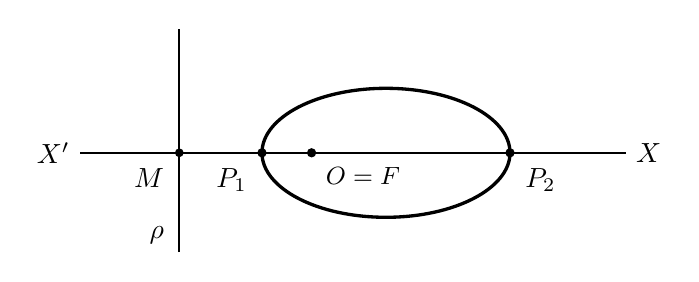
\begin{tikzpicture}[scale=1.05]
  % Directrix \rho at x = -1.6
  \draw[thick] (-1.6, -1.2) -- (-1.6, 1.5);
  \node[left=2pt] at (-1.6, -1.0) {$\rho$};

  % Horizontal line X'X
  \draw[thick] (-2.8, 0) node[left] {$X'$} -- (3.8, 0) node[right] {$X$};

  % Intersection M
  \fill (-1.6, 0) circle (1.5pt) node[below left=2pt] {$M$};

  % Ellipse: P_1 at -0.6, P_2 at 2.4, center at 0.9, x radius = 1.5, y radius = 0.78
  \draw[very thick] (0.9, 0) ellipse [x radius=1.5, y radius=0.78];

  % Points P_1, O=F, P_2
  \fill (-0.6, 0) circle (1.6pt);
  \node[below left=2pt] at (-0.6, 0) {$P_1$};

  \fill (0, 0) circle (1.6pt);
  \node[below right=1pt, font=\small] at (0.02, -0.02) {$O=F$};

  \fill (2.4, 0) circle (1.6pt);
  \node[below right=2pt] at (2.4, 0) {$P_2$};
\end{tikzpicture}
\caption*{圖 5-3}
\label{fig:b5-5-3}
\end{figure}

\noindent
\textbf{注意}\quad $P_1$ 與 $P_2$ 一在 $OM$ 之間，一在 $O$ 的右側，而同在 $\rho$ 的右側，這一觀察正是 $\Gamma$ 為橢圓時，如圖 5-3，所應有的現象．

\paragraph*{(ii) \underline{當 $e = 1$ 時}}
在水平軸 $X'X$ 上，$\Gamma$ 只交一次且正好是線段 $OM$ 的中點．

\begin{figure}[H]
\centering
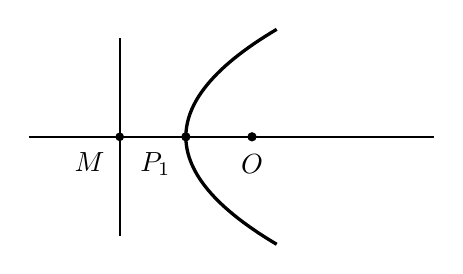
\begin{tikzpicture}[scale=1.05]
  % Directrix \rho at x = -1.6
  \draw[thick] (-1.6, -1.2) -- (-1.6, 1.2);

  % Horizontal axis X'X
  \draw[thick] (-2.7, 0) -- (2.2, 0);

  % Point M at (-1.6, 0), O at (0, 0), P_1 at (-0.8, 0)
  \fill (-1.6, 0) circle (1.5pt) node[below left=2pt] {$M$};
  \fill (-0.8, 0) circle (1.6pt) node[below left=2pt] {$P_1$};
  \fill (0, 0) circle (1.6pt) node[below=3pt] {$O$};

  % Parabola opening right with vertex at P_1(-0.8, 0)
  \draw[very thick, domain=-1.3:1.3, samples=60]
    plot ({-0.8 + 0.65*(\x)^2}, {\x});
\end{tikzpicture}
\caption*{圖 5-4}
\label{fig:b5-5-4}
\end{figure}

\paragraph*{(iii) \underline{當 $e > 1$ 時}}
在水平軸 $X'X$ 上，$\Gamma$ 交 $X'X$ 兩次，其一仍在 $O$ 與 $M$ 之間，另一則反落到 $M$ 的左側（或 $\rho$ 的左側）．

\begin{figure}[H]
\centering
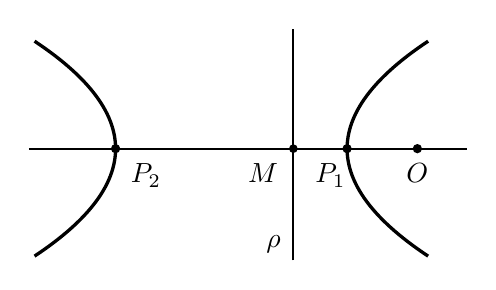
\begin{tikzpicture}[scale=1.05]
  % Directrix \rho at x = 0
  \draw[thick] (0, -1.35) -- (0, 1.45);
  \node[left=1pt] at (0, -1.15) {$\rho$};

  % Horizontal line X'X
  \draw[thick] (-3.2, 0) -- (2.1, 0);

  % Points P_2, M, P_1, O
  \fill (0, 0) circle (1.5pt) node[below left=2pt] {$M$};
  \fill (0.65, 0) circle (1.6pt);
  \node[below=2pt] at (0.45, 0) {$P_1$};
  \fill (1.5, 0) circle (1.6pt) node[below=2pt] {$O$};
  \fill (-2.15, 0) circle (1.6pt);
  \node[below right=2pt] at (-2.15, 0) {$P_2$};

  % Right branch through P_1(0.65, 0) opening right
  \draw[very thick, domain=-1.3:1.3, samples=60]
    plot ({0.65 + 0.58*(\x)^2}, {\x});

  % Left branch through P_2(-2.15, 0) opening left
  \draw[very thick, domain=-1.3:1.3, samples=60]
    plot ({-2.15 - 0.58*(\x)^2}, {\x});
\end{tikzpicture}
\caption*{圖 5-5}
\label{fig:b5-5-5}
\end{figure}

\subsubsection*{作業 14}
一直線 $L$ 上兩點 $M$ 與 $O$，試在 $L$ 上找出滿足 $\dfrac{PO}{PM} = \dfrac{1}{3}$ 的點，描於 $L$ 上，並注意其與 $O$ 的相關位置（在 $O$ 之左側或右側？）

\subsubsection*{作業 15}
用極圖觀點驗證
\[
  \begin{cases}
    r = \dfrac{pe}{1 - e\cos\theta} \\[0.6em]
    \theta = 0
  \end{cases}
\]
有兩解 $\left(\dfrac{pe}{1-e}, 0\right)$ 與 $\left(\dfrac{pe}{1+e}, 0\right)$\phantomsection\label{note:b5-ch1-p48-hw15}\footnote{【原書註記/校訂】：原書此處聯立條件印作「$\theta = 0$」，兩解印作「$\left(\frac{pe}{1-e}, 0\right)$ 與 $\left(\frac{pe}{1+e}, 0\right)$」，緊接解釋「換句話說第二解 $r$ 為負值其實就在 $\theta = \pi$ 的方向上」．按極平面上直線 $X'X$ 包含 $\theta = 0$ 與 $\theta = \pi$ 兩方向：當 $\theta = \pi$ 時代入極方程式得 $r = \frac{pe}{1 - e\cos\pi} = \frac{pe}{1+e}$，對應極座標為 $\left[\frac{pe}{1+e}, \pi\right]$；若改以 $\theta = 0$ 表示同一點，則其 $r$ 值為負，即 $\left[-\frac{pe}{1+e}, 0\right]$．原書於第二解漏印負號（或將角度 $\pi$ 誤印為 $0$），特此註明．}．換句話說第二解 $r$ 為負值其實就在 $\theta = \pi$ 的方向上，故 $\Gamma$ 與 $X'X$ 的兩交點分居於 $O$ 的兩側．

\subsubsection*{作業 16}
仿作業 14，直觀地看看是否 $L$ 上到 $O$ 點與到 $M$ 點等距離的點果真只有 $OM$ 中點？

\subsubsection*{作業 17}
仿\underline{作業 15} 驗證 $\Gamma$ 只交 $X'X$ 於 $OM$ 中點．

\subsubsection*{作業 18}
仿作業 14, 15 解釋 (iii) 中所述．

\subsubsection*{作業 19}
用極圖觀點證明：任一通過焦點的直線（水平線除外）與拋物線：
\[
  r = \frac{p}{1 - \cos\theta}
\]
都正好有兩個交點．

\subsubsection*{作業 20}
一通過焦點的直線與單支雙曲線的交點有幾個？從這件事你能否定義出所謂「開口」的角度，而得到拋物線的開口 $= 0$，恒小於雙曲線的開口？

\begin{example-non}[【論例 5】]
\underline{刻卜勒}（Kepler）第一定律說：行星繞太陽旋轉的軌道是一個以太陽為焦點的橢圓，第二定律則說：對於一固定行星，在同一時間區段內，此行星對太陽所掃出的近似扇形的面積相等，此卽為\underline{天體運動說}．從這裏你可以推論「行星運行的速度（不計其方向）在近日點時，與在遠日點時相較，那一時候快？」（作業 21）

\begin{figure}[H]
\centering
\begin{tikzpicture}[scale=1.05]
  % Ellipse centered at (0,0) with a = 2.4, b = 0.85
  % Focus (Sun) at (-1.45, 0)
  \coordinate (Sun) at (-1.45, 0);
  \coordinate (Peri) at (-2.4, 0);
  \coordinate (Aphe) at (2.4, 0);

  % Shaded sector 1 near Perihelion: from angle 152 to 205 on ellipse
  \begin{scope}
    \path[clip] (Sun) -- ({2.4*cos(152)}, {0.85*sin(152)})
      arc [start angle=152, end angle=205, x radius=2.4, y radius=0.85] -- cycle;
    \foreach \x in {-3.0, -2.9, ..., -1.0} {
      \draw[thin, gray!80!black] (\x, -1.0) -- (\x+1.2, 1.0);
    }
  \end{scope}
  \draw[thick] (Sun) -- ({2.4*cos(152)}, {0.85*sin(152)});
  \draw[thick] (Sun) -- ({2.4*cos(205)}, {0.85*sin(205)});

  % Shaded sector 2 towards Aphelion (upper right): from angle 42 to 72 on ellipse
  \begin{scope}
    \path[clip] (Sun) -- ({2.4*cos(42)}, {0.85*sin(42)})
      arc [start angle=42, end angle=72, x radius=2.4, y radius=0.85] -- cycle;
    \foreach \x in {-1.8, -1.7, ..., 2.2} {
      \draw[thin, gray!80!black] (\x, -1.0) -- (\x+1.2, 1.0);
    }
  \end{scope}
  \draw[thick] (Sun) -- ({2.4*cos(42)}, {0.85*sin(42)});
  \draw[thick] (Sun) -- ({2.4*cos(72)}, {0.85*sin(72)});

  % Ellipse outline
  \draw[very thick] (0, 0) ellipse [x radius=2.4, y radius=0.85];

  % Dots for Sun, Perihelion, Aphelion
  \fill (Sun) circle (2.5pt);
  \node[below right=1pt] at (-1.35, 0.05) {\small 太陽};

  \fill (Peri) circle (2pt);
  \node[left=4pt, align=center] at (Peri) {\small 近\\[-2pt]\small 日\\[-2pt]\small 點};

  \fill (Aphe) circle (2pt);
  \node[right=4pt] at (Aphe) {\small 遠日點};
\end{tikzpicture}
\caption*{圖 5-6}
\label{fig:b5-5-6}
\end{figure}

但注意由於運行速度不均勻，這裏我們所說的“速度”的意義也似乎不明，這便是到了\underline{牛頓}時代所產生的前兆微分觀念．
\end{example-non}

\subsubsection*{作業 21}
上文同一行星的運行速度，離太陽越遠越快，還是越近越快？（暫且粗略判斷）

\subsubsection*{丙、決定形狀的資料}

在極方程式中，$p$ 與 $e$ 一旦決定，二次曲線的形狀也就決定，若非拋物線，則 $\{p, e\}$ 這組資料又可換成 $\{a, c\}$ 其中 $a$ 為長軸或貫軸半長，$c$ 為兩焦點間距半長，如

橢圓時，
\[
  \begin{cases}
    p = \dfrac{a}{e}(1 - e^2) = \dfrac{a^2}{c} - c \\[0.8em]
    e = \dfrac{c}{a}
  \end{cases}
\]

雙曲線時，
\[
  \begin{cases}
    p = \dfrac{a}{e}(e^2 - 1) = c - \dfrac{a^2}{c} \\[0.8em]
    e = \dfrac{c}{a}
  \end{cases}
\]

\subsubsection*{作業 22}
將上式換算式詳加驗證，並討論拋物線的情形．

\subsubsection*{丁、旋轉}

對於一個開口朝左的拋物線，我們是否稍一觀察就能利用開口朝右極方程式 \eqref{eq:b5-1-5-1}（其中取 $e = 1$）
\[
  r = \frac{p}{1 - \cos\theta}
\]
而寫下開口朝左的極方程式？

方法由下圖 5-7

\begin{figure}[H]
\centering
\begin{tikzpicture}[scale=1.0]
  % ==================== Left Subfigure: Opening Left ====================
  \begin{scope}[shift={(-3.5, 0)}]
    \draw[thick, -Stealth] (-2.3, 0) -- (2.1, 0) node[below] {$X$};
    \draw[thick, -Stealth] (0, -1.7) -- (0, 1.9) node[right] {$Y$};

    % Parabola opening left: r = p / (1 + cos\theta), p = 0.85
    \draw[very thick, domain=-122:122, samples=80]
      plot ({0.85/(1 + cos(\x))*cos(\x)}, {0.85/(1 + cos(\x))*sin(\x)});

    % Ray in 3rd quadrant at \theta = 240 deg
    \pgfmathsetmacro{\thL}{240}
    \pgfmathsetmacro{\rL}{0.85/(1 + cos(\thL))}
    \coordinate (PL) at ({\rL*cos(\thL)}, {\rL*sin(\thL)});
    \draw[thick] (0, 0) -- (PL);

    % Angle arc for \theta
    \draw[thick] (0.32, 0) arc (0:\thL:0.32);
    \node at (-0.28, 0.50) {\small $\theta$};

    % Label r
    \node at (-0.62, -0.58) {$r$};
  \end{scope}

  % ==================== Right Subfigure: Opening Right ====================
  \begin{scope}[shift={(3.0, 0)}]
    \draw[thick, -Stealth] (-1.9, 0) -- (2.5, 0) node[below] {$X$};
    \draw[thick, -Stealth] (0, -1.7) -- (0, 1.9) node[right] {$Y$};

    % Parabola opening right: r_1 = p / (1 - cos\theta_1), p = 0.85
    \draw[very thick, domain=58:302, samples=80]
      plot ({0.85/(1 - cos(\x))*cos(\x)}, {0.85/(1 - cos(\x))*sin(\x)});

    % Ray in 1st quadrant at \theta_1 = 60 deg
    \pgfmathsetmacro{\thR}{60}
    \pgfmathsetmacro{\rR}{0.85/(1 - cos(\thR))}
    \coordinate (PR) at ({\rR*cos(\thR)}, {\rR*sin(\thR)});
    \draw[thick] (0, 0) -- (PR);

    % Angle arc for \theta_1
    \draw[thick] (0.35, 0) arc (0:\thR:0.35);
    \node at (0.55, 0.25) {\small $\theta_1$};

    % Label r_1 cleanly to the left of the ray in Q1
    \node at (0.25, 0.80) {\small $r_1$};

    % Equation label and curved pointer to upper right branch
    \node[right] at (1.38, 1.62) {\small $r_1 = \dfrac{p}{1 - \cos\theta_1}$};
    \draw[thick, -Stealth] (1.36, 1.55) to[out=205, in=70] (1.10, 1.25);
  \end{scope}
\end{tikzpicture}
\caption*{圖 5-7}
\label{fig:b5-5-7}
\end{figure}

討論如下：

只要左右兩圖相較，左圖之 $\theta$ 減去 $\pi$ 後記為 $\theta_1$，則相應的，
\[
  r = r_1 = \frac{p}{1 - \cos\theta_1}
\]
故
\[
  r = \frac{p}{1 - \cos(\theta - \pi)}
\]
卽
\[
  r = \frac{p}{1 + \cos\theta}
\]
\underline{一般的情形一樣}，例如一個橢圓其長軸的傾斜角為 $\theta_0$，則其極方程式由下圖 5-8

\begin{figure}[H]
\centering
\begin{tikzpicture}[scale=1.1]
  % ==================== Left Subfigure: Tilted Ellipse ====================
  \begin{scope}[shift={(-3.5, 0)}]
    \draw[thick, -Stealth] (-1.9, 0) -- (2.3, 0) node[right] {$X$};
    \draw[thick, -Stealth] (0, -1.6) -- (0, 2.15) node[above] {$Y$};

    % Major axis line at \theta_0 = 46 deg
    \draw[thick] (226:1.85) -- (46:2.45);

    % Tilted ellipse with focus at (0,0), center shifted by 0.52 along 46 deg
    % x radius = 1.55, y radius = 0.85
    \begin{scope}[rotate=46]
      \draw[very thick] (0.52, 0) ellipse [x radius=1.55, y radius=0.85];
    \end{scope}

    % Angle arc for \theta_0 (0 to 46 deg) at radius 0.36
    \draw[thick, -Stealth] (0.36, 0) arc (0:46:0.36);
    \node at (21:0.58) {\footnotesize $\theta_0$};

    % Ray at angle \theta = 104 deg (in Q2)
    \coordinate (Ptilted) at (104:1.00);
    \draw[thick] (0, 0) -- (Ptilted);

    % Angle arc for \theta (0 to 104 deg) at radius 0.82 (outside \theta_0!)
    \draw[thick, -Stealth] (0.82, 0) arc (0:104:0.82);
    \node at (75:1.02) {\small $\theta$};

    % Label r clearly inside the ellipse to the left of the ray in Q2
    \node at (130:0.48) {\small $r$};
  \end{scope}

  % ==================== Middle Rotation Arrow & Formula ====================
  \draw[thick, -Stealth] (-1.15, 0.95) to[bend left=18] node[midway, above=2pt] {\small 轉 $\theta_0$ 角} (0.95, 0.95);
  \node at (-0.10, -1.25) {$(\theta - \theta_0 = \theta_1)$};

  % ==================== Right Subfigure: Horizontal Ellipse ====================
  \begin{scope}[shift={(3.0, 0)}]
    \draw[thick, -Stealth] (-1.5, 0) -- (2.6, 0) node[right] {$X$};
    \draw[thick, -Stealth] (0, -1.6) -- (0, 2.15) node[above] {$Y$};

    % Horizontal ellipse with focus at (0,0)
    \draw[very thick] (0.52, 0) ellipse [x radius=1.55, y radius=0.85];

    % Ray at angle \theta_1 = 58 deg
    \coordinate (Phoriz) at (58:1.00);
    \draw[thick] (0, 0) -- (Phoriz);

    % Angle arc for \theta_1
    \draw[thick, -Stealth] (0.42, 0) arc (0:58:0.42);
    \node at (26:0.65) {\footnotesize $\theta_1$};

    % Label r_1 cleanly inside the ellipse between Y-axis and ray
    \node at (75:0.56) {\footnotesize $r_1$};
  \end{scope}
\end{tikzpicture}
\caption*{圖 5-8}
\label{fig:b5-5-8}
\end{figure}

得
\[
  r = r_1 = \frac{pe}{1 - e\cos\theta_1} = \frac{pe}{1 - e\cos(\theta - \theta_0)}\phantomsection\label{note:b5-ch1-p51-eq}\footnote{【原書註記/校訂】：原書此式第一個分式前之等號上橫畫漏印，致外觀形似減號「$r = r_1 - \frac{pe}{1 - e\cos\theta_1}$」，按上頁同構推導應為等號「$r = r_1 = \frac{pe}{1 - e\cos\theta_1}$」，茲予校訂．}
\]
卽
\[
  r = \frac{pe}{1 - e\cos(\theta - \theta_0)}
\]

\subsubsection*{作業 23}
設有一雙曲線，貫軸半長 $a = 1$，焦點在原點，兩焦距間半長 $c = 3$，且貫軸傾斜角為 $\dfrac{2\pi}{3}$，求其極方程式．（先求 $p, e$ 再利用旋轉）

\subsubsection*{戊、換成直角座標方程式}

今已知二次曲線的極方程式為
\begin{equation}
  r = \frac{pe}{1 - e\cos\theta} \tag{2} \label{eq:b5-1-5-2}
\end{equation}
將它換成直角座標方程式如下：
\begin{align}
  r - re\cos\theta &= pe \nonumber \\
  r &= e(p + r\cos\theta) \nonumber \\
  r^2 &= e^2(p + r\cos\theta)^2 \tag{3} \label{eq:b5-1-5-3}
\end{align}
表面上因平方所引入的增式 $r = -e(p + r\cos\theta)$ $\left(\text{或等價地 } r = \dfrac{-pe}{1 + e\cos\theta}\right)$，會引進增解 $\left[\dfrac{-pe}{1 + e\cos\theta}, \theta\right]$，但由於當 $\theta$ 繞半圈成 $\theta + \pi$ 時，$r$ 亦取值為 $\dfrac{pe}{1 + e\cos\theta}$，亦卽
\[
  \left[\frac{pe}{1 + e\cos\theta}, \theta + \pi\right] = \left[\frac{-pe}{1 + e\cos\theta}, \theta\right]
\]
而使 \eqref{eq:b5-1-5-3} 式不因平方增添任何多餘的新點．（見\underline{作業 24}）則
\[
  x^2 + y^2 = e^2(p + x)^2
\]

\subsubsection*{作業 24}
一般一個
\[
  r = f(r\cos\theta, r\sin\theta)
\]
的極方程式（自為良性），經兩端平方後在極平面上所代表的軌跡不變．其道理的要點已如上文，試述其詳．

〔提示：$r = -f(r\cos\theta, r\sin\theta)$，若 $[r_1, \theta_1]$ 滿足 $r = f(r\cos\theta, r\sin\theta)$，則 $[-r_1, \theta_1 + \pi]$ 滿足 $r = -f(r\cos\theta, r\sin\theta)$〕

% =========================================================================
% 習題 I-5
% =========================================================================
\subsubsection*{習題 I-5}
\label{sec:b5-ex1-5}

\begin{enumerate}[1.]
  \item 判別下列各極方程式在極平面上屬何種軌跡？並描畫其圖．
  \begin{multicols}{2}
  \begin{enumerate}[(a)]
    \item $r(4 - 5\cos\theta) = 7$
    \item $r(2 + \sqrt{3}\cos\theta) = 3$
    \item $r = \dfrac{1}{8(1 - \cos\theta)}$
    \item $r^2\cos 2\theta = 10$
  \end{enumerate}
  \end{multicols}

  \item
  \begin{enumerate}[(a)]
    \item 描繪極平面上
    \begin{multicols}{2}
    \begin{enumerate}[(i)]
      \item $r = \dfrac{2}{2 - \sin\theta}$
      \item $r = \dfrac{1}{1 - 2\sin\theta}$
      \item $r = \dfrac{1}{1 + \sin\theta}$
      \item $r = \dfrac{1}{1 - \sin\theta}$
    \end{enumerate}
    \end{multicols}
    之軌跡．
    \item 取原點為焦點，不過原點而平行極軸的一直線為準線，試證所得的二次曲線之極方程式為
    \[
      r = \frac{pe}{1 \pm e\sin\theta}
    \]
    並決定何時式中取正，何時取負．

    〔採用 (i) 仿本文直接導引，(ii) 旋轉取 $\dfrac{\pi}{2} - \theta$ 以代本文中 \eqref{eq:b5-1-5-1} 式〕
  \end{enumerate}

  \item 已知某橢圓極方程式為
  \[
    r = \frac{20}{3 - 2\cos\theta}
  \]
  試求其離心率，兩焦點之位置〔以直角座標描述〕，長軸、短軸之半長，及準線位置．

  \item 極平面上一個二次曲線若知以原點為焦點，以
  \[
    2x + y + 4 = 0
  \]
  為準線，求此時二次曲線的極方程式（離心率 $e$ 已知）．

  〔提示：將本文 \eqref{eq:b5-1-5-1} 式作一旋轉〕

  \item 設極平面上一個以原點為焦點的二次曲線上含 $P_1[2, \alpha]$, $P_2\left[4, \dfrac{\pi}{2} + \alpha\right]$, $P_3[8, \pi + \alpha]$ 三點，求其離心率．

  \item 一連結二次曲線上兩點之線段，若通過焦點 $F$ 稱為\textbf{焦弦}．試證對二次曲線
  \[
    r = \frac{pe}{1 - e\cos\theta}
  \]
  上任一焦弦 $PP'$，恒有
  \[
    \frac{1}{\overline{FP}} + \frac{1}{\overline{FP'}} = \frac{2}{pe}
  \]

  \item 適當取一極座標用以描寫“到兩定點乘積一定”之曲線〔雙紐線〕，並問這種曲線用直角座標表示時最低須為幾次？

  \item 若以有心錐線的中心為極點，軸為極軸，$e$ 為離心率，$b$ 為短軸（或共軛軸）之半長，則

  橢圓的極方程式呈 $r^2 = \dfrac{b^2}{1 - e^2\cos^2\theta}$ 型式，

  双曲線的極方程式呈 $r^2 = \dfrac{b^2}{e^2\cos^2\theta - 1}$ 型式．試驗證之．

  \item[*9.] 二次錐線 $2x^2 + 2xy + y^2 = 1$ 上之三點 $P, Q, R$ 與原點 $O$ 滿足 $\angle POQ = \angle QOR = \angle ROP$，則試導證出
  \[
    \frac{1}{\overline{OP}^2} + \frac{1}{\overline{OQ}^2} + \frac{1}{\overline{OR}^2} \quad \text{一式之值}
  \]
  與 $P, Q, R$ 三點的相對位置無關．

  \item[10.]
  \begin{enumerate}[(a)]
    \item 試化 $r = \dfrac{1}{2}\tan\theta$ 為直角座標方程式，並描其軌跡．
    \item 試化 $(x^2 + y^2)^2 = a^2(x^2 - y^2)$ 為極方程式，並描其軌跡 $[a \neq 0]$．
  \end{enumerate}
\end{enumerate}

% =========================================================================
% § I-6 極圖映射下面積的變化率
% =========================================================================
\subsection{極圖映射下面積的變化率}
\label{sec:b5-1-6}

\begin{figure}[H]
\centering
\begin{tikzpicture}[scale=1.08]
  % ==================== Left: (\theta, r)-plane ====================
  \begin{scope}[shift={(-3.5, 0)}]
    \draw[thick, -Stealth] (-0.9, 0) -- (3.3, 0) node[right] {$\theta$};
    \draw[thick, -Stealth] (0, -0.75) -- (0, 2.35) node[right] {$r$};

    % Rectangle A
    \draw[very thick] (0.75, 0.95) rectangle (1.65, 1.48);
    \node at (1.2, 1.215) {$A$};

    % Dimension labels \Delta\theta and \Delta r
    \node[below=2pt] at (1.2, 0.95) {\small $\Delta\theta$};
    \node[left=2pt] at (0.75, 1.215) {\small $\Delta r$};

    % Corner labels
    \node[above right=1pt] at (1.60, 1.48) {\small $(\theta + \Delta\theta, r + \Delta r)$};
    \node (thr) at (-0.52, 0.42) {\small $(\theta, r)$};
    % Curved leader from (\theta, r) to lower-left corner (0.75, 0.95)
    \draw[thick] (thr.east) .. controls (0.35, 0.55) and (0.20, 0.72) .. (0.42, 0.78)
      .. controls (0.60, 0.83) and (0.35, 0.88) .. (0.75, 0.95);
  \end{scope}

  % ==================== Middle Mapping Arrow \gamma ====================
  \draw[thick, -Stealth] (0.45, 0) -- node[above=2pt] {$\gamma$} (1.35, 0);

  % ==================== Right: (x, y)-plane ====================
  \begin{scope}[shift={(2.3, 0)}]
    \draw[thick, -Stealth] (-0.85, 0) -- (3.3, 0) node[right] {$x$};
    \draw[thick, -Stealth] (0, -0.75) -- (0, 2.45) node[right] {$y$};

    % Two rays at \theta_a = 30 deg and \theta_b = 60 deg
    \pgfmathsetmacro{\tha}{30}
    \pgfmathsetmacro{\thb}{60}
    \pgfmathsetmacro{\rOne}{1.60}
    \pgfmathsetmacro{\rTwo}{2.38}

    \draw[thick] (0, 0) -- (\tha:\rOne);
    \draw[thick] (0, 0) -- (\thb:\rOne);

    % Annular sector B
    \draw[very thick] (\tha:\rOne) -- (\tha:\rTwo)
      arc (\tha:\thb:\rTwo) -- (\thb:\rOne)
      arc (\thb:\tha:\rOne) -- cycle;

    \node at (45:1.99) {$B$};
    \node at (45:1.10) {\small $\Delta\theta$};
    \node at (22:2.05) {\small $\Delta r$};
    \node[above right=2pt] at (46:\rTwo) {\small $r\Delta\theta$};

    % Corner label [r, \theta] clearly below (\tha:\rOne) = (1.386, 0.80)
    \node (rth) at (1.88, 0.36) {\small $[r, \theta]$};
    \draw[thick] (rth.north west) .. controls (1.42, 0.62) and (1.44, 0.72) .. (\tha:\rOne);
  \end{scope}
\end{tikzpicture}
\caption*{圖 6-1}
\label{fig:b5-6-1}
\end{figure}

上圖中若在 $(\theta, r)$—平面上 $\theta$ 與 $r$ 各自增加 $\Delta\theta$ 與 $\Delta r$，而考慮矩形 $A$（$A$ 之面積仍記以 $A$），另一方面經過極圖映射 $\gamma$ 後，矩形 $A$ 變成扇形靠底的一部份 $B$（$B$ 之面積仍記以 $B$）．

現在我們來計算 $B : A$ 的比值，$A$ 易知為 $A = (\Delta r)\Delta\theta$，$B$ 為大扇形與小扇形之差，故
\begin{align*}
  B &= \frac{1}{2}(r + \Delta r)^2\Delta\theta - \frac{1}{2}r^2\Delta\theta \\
    &= \frac{1}{2}(2r\Delta r + (\Delta r)^2)\Delta\theta = r\Delta r\Delta\theta + \frac{1}{2}(\Delta r)^2\Delta\theta
\end{align*}
故
\[
  \frac{B}{A} = r + \frac{1}{2}\Delta r
\]
當增量 $\Delta r \longrightarrow 0$ 時
\[
  \frac{B}{A} \longrightarrow r
\]
這表示極圖映射下面積的漲縮率隨 $r$ 值而變動．下圖 6-2 可以幫助我們了解：

\begin{figure}[H]
\centering
\begin{tikzpicture}[scale=1.08]
  % ==================== Left: (\theta, r)-plane ====================
  \begin{scope}[shift={(-3.7, 0)}]
    \draw[thick, -Stealth] (-1.0, 0) -- (3.4, 0) node[right] {$\theta$};
    \draw[thick, -Stealth] (0, -0.85) -- (0, 3.15) node[right] {$r$};

    % Tick mark 1 on r-axis (between A_2 and A_3)
    \draw[thick] (-0.06, 1.20) -- (0.06, 1.20);
    \node[left=2pt] at (-0.04, 1.20) {\small $1$};

    % Four congruent hatched rectangles A_1, A_2, A_3, A_4 (shifted to x in [0.70, 1.50] so labels A_i never touch the r-axis!)
    \foreach \idx/\ymin/\ymax in {1/0.26/0.56, 2/0.82/1.12, 3/1.42/1.72, 4/2.02/2.32} {
      \begin{scope}
        \path[clip] (0.70, \ymin) rectangle (1.50, \ymax);
        \foreach \x in {0.77, 0.85, ..., 1.48} {
          \draw[thin] (\x, \ymin) -- (\x, \ymax);
        }
      \end{scope}
      \draw[thick] (0.70, \ymin) rectangle (1.50, \ymax);
      \node[left=1pt] at (0.70, {0.5*(\ymin+\ymax)}) {\small $A_{\idx}$};
    }

    % Unhatched rectangle A at same height as A_3
    \draw[thick] (2.15, 1.42) rectangle (2.95, 1.72);
    \node[right=2pt] at (2.95, 1.57) {\small $A$};
  \end{scope}

  % ==================== Middle Mapping Arrow \gamma ====================
  \draw[thick, -Stealth] (0.25, 0.75) -- node[above=2pt] {$\gamma$} (1.25, 0.75);

  % ==================== Right: (x, y)-plane ====================
  \begin{scope}[shift={(2.45, 0)}]
    \draw[thick, -Stealth] (-1.0, 0) -- (3.8, 0) node[right] {$x$};
    \draw[thick, -Stealth] (0, -0.85) -- (0, 3.15) node[above] {$y$};

    % Rays at \theta_1 = 35 deg and \theta_2 = 55 deg
    \pgfmathsetmacro{\thOne}{35}
    \pgfmathsetmacro{\thTwo}{55}
    \draw[thick] (0, 0) -- (\thOne:3.65);
    \draw[thick] (0, 0) -- (\thTwo:3.65);

    % Four hatched annular sectors B_1, B_2, B_3, B_4
    \foreach \idx/\rmin/\rmax in {1/0.35/0.65, 2/0.92/1.22, 3/1.50/1.86, 4/2.12/2.46} {
      \begin{scope}
        \path[clip] (\thOne:\rmin) -- (\thOne:\rmax)
          arc (\thOne:\thTwo:\rmax) -- (\thTwo:\rmin)
          arc (\thTwo:\thOne:\rmin) -- cycle;
        \foreach \ang in {37.5, 40.0, ..., 53.5} {
          \draw[thin] (0, 0) -- (\ang:2.6);
        }
      \end{scope}
      \draw[thick] (\thOne:\rmin) -- (\thOne:\rmax)
        arc (\thOne:\thTwo:\rmax) -- (\thTwo:\rmin)
        arc (\thTwo:\thOne:\rmin) -- cycle;
    }

    % Dashed concentric arcs at r = 1.50 and r = 1.86 connecting x-axis through B_3 to B
    \draw[dashed] (0:1.50) arc (0:76:1.50);
    \draw[dashed] (0:1.86) arc (0:76:1.86);

    % Cleanly offset labels B_1, B_2, B_3, B_4 below the lower ray (35 deg) with white halo
    \node at (18:0.55) {\footnotesize $B_1$};
    \node at (20:1.08) {\footnotesize $B_2$};
    \node[fill=white, inner sep=1pt] at (21:1.68) {\footnotesize $B_3$};
    \node at (22:2.30) {\footnotesize $B_4$};

    % Tick mark 1 on x-axis
    \node[below=2pt] at (1.25, 0) {\small $1$};

    % Unhatched annular sector B at same radius as B_3 (r in [1.50, 1.86]), angle [76, 96]
    \draw[thick] (76:1.50) -- (76:1.86)
      arc (76:96:1.86) -- (96:1.50)
      arc (96:76:1.50) -- cycle;
    \node[left=2pt] at (96:1.68) {\small $B$};
  \end{scope}
\end{tikzpicture}
\caption*{圖 6-2}
\label{fig:b5-6-2}
\end{figure}

\noindent
\textbf{圖說：} $r$ 值增大，面積也越漲越大（如 $A_1 = A_2 = A_3 = A_4$ 而 $B_1, B_2, B_3, B_4$ 越來越大），$r$ 值相同，$\theta$ 值變動，面積漲縮率不變（如 $A = A_3$，而 $B$ 亦 $= B_3$）．
